We have the sense in the previous chapters that we want to study some distributions when our matrices are large enough - be that for feasibility of computations or approximation of infinite dimension operators. We also have mentioned that our main interest here is in Invariant Ensembles, or specially in orthogonal polynomial ones. Because of this, studying large matrices is equivalent, in some sense, to studying the regime of large $N$ for orthogonal polynomials. For some of those polynomials, a integral representation is available, allowing us to use asymptotic methods on integrals to solve for the large $N$ behavior. This is the main discussion of this chapter.

\section{Quadrature Technique}

Before doing asymptotics on integrals we discuss a technique that will become important when approximating large summations: quadratures, i.e., approximating integrals by summations and vice-versa. One can see that asymptotics on integrals can then also perform a role on discrete summations. We first start briefly introducing a useful tool in the development of the formula we wish to use: the Bernoulli numbers $B_n$, polynomials $B_n(x)$ and periodic polynomials $\tilde{B}_n(x)$. The Bernoulli numbers $B_n$ are a sequence of rational numbers that frequently appears in the Taylor series expansion of trigonometric-type functions. These number can also be seen as special values obtained by the Bernoulli polynomials $B_n(x)$. This is because these polynomials can be written explicitly as
\begin{equation}
	B_k(x) = \sum_{n=0}^{k} {k \choose n} B_n x^{k-n},
\end{equation}
then, we must have that $B_k(0) = B_k$. More interestingly for us is the fact that these polynomials satisfy the differential equation 
\begin{equation}
	B'_n(x) = n B_{n-1}(x), \quad n = 1,2,\cdots
	\label{Equation: Differential Bernoulli}
\end{equation}
Finally, the periodic Bernoulli polynomial is simply the Bernoulli polynomials evaluated at the fractional part of the argument, i.e., $\tilde{B}_n(x) = B_n(x - \floor{x})$. Now, let $B_n$ and $B_n(x)$ denote the $n$th Bernoulli number and polynomial, respectively, and $\tilde{B}_n(x)$ the $n$th Bernoulli periodic function $B_n(x - \floor{x})$. Assume that $a, m$ and $n$ are integers such that $n > a$, $m > 0$, and $f^{(2m)}(x)$ is absolutely integrable over $[a,n]$. Then, 

\begin{teorema} (Euler-Maclaurin Formula,  \cite{NISTMathFunc})
	Following the context given above, 
	\begin{multline}
		\sum_{j=a}^{n} f(j) = \int_{a}^{n} f(x) \dd x + \frac{1}{2} \left(f(a) + f(n)\right) + \sum_{s=1}^{m-1} \frac{B_{2s}}{(2s)!} \left( f^{(2s-1)}(n) - f^{(2s-1)}(a)\right) \\ + \int_{a}^{n} \frac{B_{2m} - \tilde{B}_{2m}(x)}{(2m)!} f^{(2m)}(x) \dd x.
	\end{multline}
\end{teorema}


This equation is called the \textit{Euler-Maclaurin} formula. It can be extremely useful when estimating the asymptotic of the summation on the function $f$ when its integral can be more easily evaluate. In essence, this is a quadrature technique; a numerical integration: the approximation of an integral $\int f(x) \dd x$ of some function $f$ by a discrete summation $\sum w_i f(x_i)$ over a set of points $x_i$ with some weight function $w_i$. For example, in the classical Riemann sums, one approximates the integral $\int f(x) \dd x$ over some interval $[a,b]$ with the limit of the summation $\sum f(x_i^*) \Delta x_i$, where $x_i^* \in [x_{i-1}, x_i]$ and $ \Delta x_i = x_i - x_{i-1}$. Different methods can be generated by choosing $x_i^*$ differently.

The trapezoidal rule, for example, is a Riemann sum where $x_i^*$ is chosen to be the mean point $x_i^* = (x_{i-1} + x_i)/2$. In this way, we would estimate the area using trapezoids, as the name suggests. Then, one could write
\begin{align}
	\int_{a}^{n} f(x) \dd x & \approx \sum_{j = 0}^{n} f(x_j^*) = \sum_{j = 0}^{n} \frac{f(x_{i} + x_{i-1})}{2}, \\
	& = \sum_{j = 1}^{n-1} f(x_j^*) + \frac{1}{2} \left( f(n) + f(0) \right) = \sum_{j = 0}^{n-1} f(x_j^*) + \frac{1}{2} \left( f(n) - f(n) \right) .
\end{align}
Of course, this has some error term. Suppose that for some $(x_i, x_{i-1})$ we have the same $k$-derivatives at both extreme points for every $k\geq 1$, i.e., the function is constant. Then, there is no error in the approximation. If however, the two extreme points differ only on the $k$th derivative, there is some curvature defined by this difference where the error comes from. Therefore, there is indication of some error function given in respect to higher order derivatives.

\begin{proof}
Following the computations in \cite{Trapezoidal-Maclaurin}, take a function $f \in C^p(\R)$ for $p \geq 1$. To derive the Euler-Maclaurin for the interval $[a,b]$, let $h = (b - a)/n$ and $c = a + j h$, then we can express
\begin{equation}
	\int_{a}^{b} f(x) \dd x = \sum_{j=0}^{n-1} \int_{a+j h}^{a+(j+1)h} f(x) \dd x
\end{equation}
where we can use the property \eqref{Equation: Differential Bernoulli} and integration by parts to rewrite each integral as
\begin{align}
	\int_{c}^{c+h} f(x) \dd x & = h \int_{0}^{1} B_0(1-x) f(c+xh) \dd x \\
	& = - h \frac{B_1(1-x)}{1!} f(c + xh) |_0^1 + h^2 \int_{0}^{1} \frac{B_1(1-x)}{1!} f'(c+xh) \dd x, \\
	& \vdots \nonumber \\
	& = - \sum_{r = 0}^{p-1} \frac{h^{r+1} B_{r+1}(1-x)}{(r+1)!} f^{(r)}(c+xh) |_0^1 + h^{p+1} \int_0^1 \frac{h^{r+1} B_{p}(1-x)}{(p)!} f^{(p)}(c+xh) \dd x, \\
	& 
	\begin{multlined}
		= h \frac{f(c) + f(c+h)}{2} - \sum_{r = 0}^{p-1} \frac{h^{r+1} B_{r+1}(1-x)}{(r+1)!} \left[ f^{(r)}(c+h) - f^{(r)}(c) \right] \\
		+ h^{p+1} \int_0^1 \frac{B_{p}(1-x)}{(p)!} f^{(p)}(c+xh) \dd x. 
	\end{multlined}
\end{align}
where one can start to notice the trapezoidal rule creeping out on the first term. Notice that it was necessary to use that $ - B_1(0) = B_1(1) = 1/2$ and $B_n(0) = B_n(1) = B_n$ for $n\neq1$. Returning to the summation, we can rearrange terms as
\begin{align}
	h & \left[ \frac{f(a)}{2} + f(a+h) + \cdots + f(b-h) + \frac{f(b)}{2} \right] = \frac{1}{2} (f(b) - f(a)) + \sum_{j=0}^{n-1} f(a + j h), \\
	& = \int_{a}^{b} f(x) \dd x + \sum_{r = 0}^{p-1} \frac{h^{r+1} B_{r+1}(1-x)}{(r+1)!} \left[ f^{(r)}(b) - f^{(r)}(a) \right] - h^{p+1} \int_0^1 \frac{B_{p}(1-x)}{(p)!} f^{(p)}(c+xh) \dd x. 
\end{align}
\end{proof}
This is the Euler-Maclaurin formula, an extension of the trapezoidal rule including the higher order terms.

\mycomment{
\section{Hermite Polynomials}

\subsection{Asymptotics for Hermite}

This example will be a collage of many sources: Check \cite{shi2021errorboundsasymptoticexpansions} and \cite{nica2025gaussianintegralformulahermite} for the main references and notation. We already know the asymptotic for $x = \boh(n)$, done in \ref{Subsection: Hermite x=n}. There are other two cases of interest that are related to methods explained in this Chapter. These are $x=\boh(1)$ and, more importantly, $x = \boh(\sqrt{n})$.

\subsubsection{Regime $x = \boh(1)$}
\label{SubSection: Hermite x=o(1)}

\begin{proposicao}
	For $x \in \R$ fixed, we have the following asymptotic as $n \rightarrow \infty$:
	\begin{equation}
		\He_n(x) = \sqrt{2} \left(\frac{n}{2}\right)^{n/2} \ee^{x^2/4} \cos{\left(\frac{n\pi}{2} - x \sqrt{n}\right)} (1 + \boh(1))
	\end{equation}
\end{proposicao}
\begin{proof}
	Start with the integral formula given by Property \ref{Def: Gaussian integral-expectation formula} and write
	\begin{align}
		\He_n(x) & = \frac{1}{\sqrt{2\pi}} \int_{-\infty}^{\infty} (x + \ii t)^n \ee^{-t^2/2} \dd t = \frac{2}{\sqrt{2\pi}} \Re\left\{ \int_{0}^{\infty} (x + \ii t)^n \ee^{-t^2/2} \dd t \right\} \\
		& = \frac{2}{\sqrt{2\pi}} \Re\left\{ \int_{\Re(z) = x, \Im(z)>0} \ee^{n\ln{(z)} + \frac{1}{2}(z-x)^2} \frac{\dd z}{\ii} \right\} \\
		& = \frac{2}{\sqrt{2\pi}} \Re\left\{ \int_{\Re(z) = 0, \Im(z)>0} \ee^{n\ln{(z)} + \frac{1}{2}(z-x)^2} \frac{\dd z}{\ii} \right\}
	\end{align}
	where you start with a line integral in $\C$ and move the contour over to the positive imaginary axis - justified by the Cauchy's Theorem and the exponential decay of the integrand near infinity. Now, we focus on $n\ln{(z)} + \frac{1}{2}(z-x)^2$ which has maximum at $z^* = \ii \sqrt{n} + \boh(\sqrt{n})$. The idea is to change variables by a factor of $\sqrt{z}$ so that the location of the maximum contribution stays $\Boh(1)$ as $n$ gets large. Specifically, we do
	\begin{equation}
		z = \ii \sqrt{n} s, \quad \frac{\dd z}{\ii} = \sqrt{n} \dd s, \quad \ln{(z)} = \ln{(\sqrt{n})} + \ln{(s)} + \ii \frac{\pi}{2}
	\end{equation}  
	which give us
	\begin{equation}
		\frac{1}{2}(z-x)^2 = -\frac{1}{2} ns^2 + \frac{1}{2} x^2 - \ii \sqrt{n} sx	
	\end{equation}
	so that we remain with
	\begin{align}
		\He_n(x) & = \frac{2}{\sqrt{2\pi}} \Re\left\{ \int_{0}^{\infty} \ee^{n\ln{(\sqrt{n})}} \ee^{n\ln{(s)}} \ee^{n\ii\frac{\pi}{2}} \ee^{\frac{1}{2}x^2}\ee^{-\ii\sqrt{n}sx} \sqrt{n} \dd s \right\} \\
		& = \frac{2}{\sqrt{2\pi}} \sqrt{n} \ee^{n\ln{(\sqrt{n})}} \ee^{\frac{1}{2}x^2}  \int_{0}^{\infty} \ee^{n\left(\ln{(s)} - \frac{1}{2}s^2 \right)} \cos{\left(n\frac{\pi}{2} - \sqrt{n} s x\right)} \dd s,
	\end{align}
	where we can apply Laplace's approximation discussed before. Noting that $\phi(s) = \ln{(s)} - \frac{1}{2}s^2$ has $\phi'(s) = \frac{1}{s} - s$ and $\phi''(s) = -\frac{1}{s^2} - 1$, with global maximum at $s^* = 1$ with $\phi(1) = \frac{1}{2}$ and $\phi''(1) = -2$, yielding
	\begin{align}
		\He_n(x) = \frac{2}{\sqrt{2\pi}} \sqrt{n} \ee^{n\ln{(\sqrt{n})}} \ee^{\frac{1}{2}x^2}  \left( \ee^{n\phi(1)} \sqrt{\frac{2\pi}{n|\phi''(1)|}} \right) \cos{\left(n\frac{\pi}{2} - \sqrt{n}x\right)} (1+\boh(1)),
	\end{align}
	which simplifies to the result.
\end{proof}

\subsubsection{Regime $x = \boh(\sqrt{n})$}

There are three asymptotics regimes for $\He_n(x)$ when $x \rightarrow \infty$ depending on the value of $\lim_{N \rightarrow \infty} x/2\sqrt{N}$ for $N = n+1$, each of which has qualitatively different behavior
\begin{itemize}
	\item Small $x$ values $-2\sqrt{N} < x < 2\sqrt{N}$: in this regime the Hermite Polynomials will be oscillating, and a have a similar qualitative behavior as \ref{SubSection: Hermite x=o(1)} with modification to phase and amplitude. These polynomials will have some connections to the \textit{arcsine law} and \textit{semi-circle law}.
	\item Large $x$ values $|x| > 2\sqrt{N}$: In this regime the polynomial doesn't have more oscillations and is monotone increasing. As $x$ grows larger, this approximation approaches \ref{Subsection: Hermite x=n}.
	\item Edge $x$ values $x = \pm 2\sqrt{N} + \Boh(N^{-\frac{1}{6}})$: in this regime the polynomials will be approximated by the Airy Function. This interpolates between the oscillatory small $x$ regime and the monotone large $x$ regimes. 
\end{itemize} 

We write the integral representation given by the Cauchy Integral applied to the Generating Function, this representation should be discussed in \ref{Subsection: Integral Hermite} and given by:
\begin{equation}
	\begin{split}
		\He_n(x) & \deff \frac{n!}{2\pi \ii} \int_{\Gamma} z^{-n-1} \ee^{xz-\frac{z^2}{2}} \dd z \\
		& = \frac{n!}{2\pi \ii} \int_{\Gamma} \ee^{xz-\frac{z^2}{2} - (n+1)\ln{(z)}} \dd z
	\end{split}
\end{equation}
Where $\Gamma$ is a contour that goes around the origin coming and going from minus infinity such as $\Gamma = \{\lambda - \ii \delta : \lambda < 0 \} \cup \{\delta \ee^{\ii \theta}: -\pi/2 < \theta < \pi/2 \} \cup \{\lambda + \ii \delta : \lambda < 0 \}$. This is equivalent to using $\Gamma = \{\ee^{\ii \theta}: 0 \leq \theta < 2\pi \}$.
\begin{figure}[h]
	\centering
	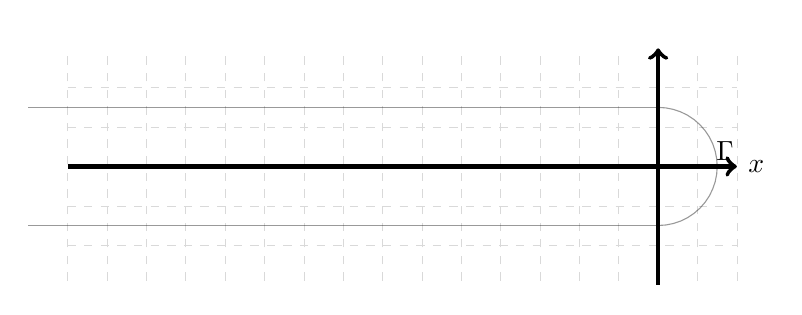
\begin{tikzpicture}[scale=.5]
		\draw[help lines, color=gray!30, dashed] (-15,-2.9) grid (2,2.9);
		\draw[->,ultra thick] (-15,0)--(2,0) node[right]{$x$};
		\draw[->,ultra thick] (0,-3)--(0,3) node[above]{$\ii$};
		
		\draw[opacity=0.4] plot[domain=-90:90] ({1.5*cos(\x)},{1.5*sin(\x)});
		\draw[opacity=0.4] plot[domain=-16:0] ({\x}, {1.5});
		\draw[opacity=0.4] plot[domain=-16:0] ({\x},{-1.5});
		
		\node (Gamma) at (1.7,0.4)    {$\Gamma$};
	\end{tikzpicture}
\end{figure}

There are a few expressions we want to have. Namely we want to determine the formulas for $\He_{n}$ and  $\He_{n-1}$.  Let's start working on the first case.  To do this, set $N = n + 1$ and consider the scaling $x \mapsto N^a \alpha$ and $z = N^b \beta$ 
\begin{equation}
	\begin{split}
		\He_n(N^a \alpha) & = \frac{(N-1)!}{2\pi \ii} \int_{\Gamma} \ee^{(N^a \alpha)(N^b \beta)- \frac{1}{2}(N^b \beta)^2 - N\ln{(N^b \beta)}} \dd \beta \\
		& \stackrel{(a = b = 1/2)}{=}   \frac{(N-1)! N^{\frac{1}{2}\left(1-N\right)}}{2\pi \ii} \int_{\Gamma}  \ee^{-N(- \alpha \beta+ \frac{1}{2} \beta^2 + \ln{(\beta)})} \dd \beta
	\end{split}
\end{equation}
So that we have
\begin{equation}
	\He_n(\sqrt{N}\alpha) = C_n^0 \int_{\Gamma}  \ee^{-N \phi_\alpha(\beta) } \dd \beta
	\label{Equation: Hermite Integral}
\end{equation}
with 
\begin{equation}
	\phi_\alpha(\beta) = \frac{1}{2} \beta^2 - \alpha \beta + \ln{(\beta)}.
\end{equation}
%The same can be done in the second case, using now the re-parametrization, that is
%\begin{equation}
%	\begin{split}
	%		\He_{n-1}(\sqrt{N} \alpha) & \stackrel{(a = b = 1/2)}{=}   \frac{n! N^{-N/4}}{2\pi \ii} \int_{\Gamma}  \ee^{-N(-2 \alpha \beta+ \beta^2 + \frac{1}{2}\ln{(\beta)})} \beta^{-1} \dd \beta
	%	\end{split}
%\end{equation}
%So that we have
%\begin{equation}	
%	\He_{n-1}(\sqrt{N}\alpha) = C_n^1 \int_{\Gamma}  \ee^{-N \phi_\alpha(\beta)} \beta^{-1} \dd \beta.
%\end{equation}
%As noted, for both cases, we have the same defining function $\phi_\alpha(\beta)$.
As we want to calculate the asymptotic by steepest descent, we need to determine the critical points of such a function and then the steepest descent paths passing through this points. We can easily determine the critical points as $\beta_c^\pm = \frac{\alpha \pm \sqrt{{\alpha}^2 - 4}}{2}$ - solutions to the quadratic formula given by solving the critical point of the function (the zeros of its derivatives). Now, the behavior of the critical points will depend on the interval of the real parameter $\alpha$. 
\begin{equation}
	\beta_c^{\pm} = \frac{\alpha \pm \sqrt{\alpha^2 - 4}}{2} =
	\begin{cases}
		\begin{aligned}
			\ee^{\pm \gamma}, \quad & \alpha = 2 \cosh{(\gamma)} > 2, \quad \gamma > 0; \\
			\ee^{\pm \ii \gamma}, \quad & \alpha = 2 \cos{(\gamma)} \in [0,2), \quad \gamma \in (0,\pi/2]; \\
			1, \quad & \alpha = 2.
		\end{aligned}
	\end{cases}
\end{equation}
Therefore, the following theorem follows.

\begin{teorema}
	The Hermite Polynomials $\He_n(x)$ have the following three representation when $x = \Boh(\sqrt{n})$ and $x > 0$:
	\begin{enumerate}
		\item Small $x$ values $-2\sqrt{N} < x < 2\sqrt{N}$: For fixed $\gamma \in (0, \pi/2)$ set $x = 2\sqrt{N} \cos{(\gamma)}$ and we obtain
		\begin{equation}
			\He_n(2\sqrt{N}\cos{(\gamma)}) = \sqrt{\frac{2}{\sin{(\gamma)}}}
			N^{\frac{1}{2} \left(N - 1\right)}
			\ee^{N\left(\cos^2{(\gamma)} - \frac{1}{2} \right)} 
			\sin{
				\left(
				\theta(\beta_c^+) 
				-N\left(\frac{\sin{(2\gamma)}}{2}
				-\gamma\right)
				\right)
			} 
			(1 + \Boh(N^{-1}))
			\label{Eq: Hermite small asymptotic (n)}
		\end{equation}
		\begin{equation}
			\He_{n-1}(2\sqrt{N}\cos(\gamma)) = \sqrt{\frac{2}{\sin{(\gamma)}}}
			N^{\frac{1}{2} \left(N -2\right)}
			\frac{\ee^{N\left(\cos^2{(\gamma)} - \frac{1}{2} \right)}}{\ee^{\cos^2{(\gamma)}}}
			\sin{
				\left(
				\theta(\beta_c^+) 
				-(N-1)\left(\frac{\sin{(2\gamma)}}{2}
				-\gamma\right)
				\right)
			} 
			(1 + \Boh(N^{-1}))
			\label{Eq: Hermite small asymptotic (n-1)}
		\end{equation}
		\item Large $x$ values $|x| > 2\sqrt{N}$: For fixed $\gamma > 1$, write $x = 2\sqrt{N} \cosh{(\gamma)}$. We obtain
		\begin{equation}
			\He_n(2\sqrt{N}\cosh{(\gamma)}) = \ee^{-N\left( \frac{\ee^{-2\gamma}}{2} + \gamma +  1\right)} \frac{N^{\frac{1}{2}\left(N - 1\right)}}{\sqrt{|1 - \ee^{2\gamma}|}} 
			\left(1 + \Boh(N^{-1}) \right),
			\label{Eq: Hermite large asymptotic (n)}
		\end{equation}
		\begin{equation}
			\He_{n-1}(2\sqrt{N}\cosh{(\gamma)}) = \frac{\ee^{-N\left( \frac{\ee^{-2\gamma}}{2} + \gamma +  1\right)}}{\ee^{\left( \frac{\ee^{-2\gamma}}{2} + \gamma + \frac{3}{2}\right)}} \frac{N^{\frac{1}{2}\left(N -2\right)}}{\sqrt{|1 - \ee^{2\gamma}|}} \left(1 + \Boh(N^{-1}) \right),
			\label{Eq: Hermite large asymptotic (n-1)}
		\end{equation}
		\item Edge $x$ values $x = \pm 2\sqrt{N} + \Boh(N^{-\frac{1}{6}})$: For fixed $u \in \R$, set x = $2\sqrt{N} + N^{-1/6}\xi$, then we obtain
		\begin{equation}
			\He_n(2\sqrt{N} + N^{-1/6}\xi) = \sqrt{2\pi\ee} N^{-\frac{N}{2} + \frac{2}{3}}  \Ai(\xi) (1 + \boh(1)),
			\label{Eq: Hermite edge asymptotic (n)}
		\end{equation}
		\begin{equation}
			\He_{n-1}(2\sqrt{N} + N^{-1/6}\xi) = \sqrt{2\pi} \ee N^{-\frac{N}{2} + \frac{7}{6}}  \Ai(\xi) (1 + \boh(1))
			\label{Eq: Hermite edge asymptotic (n-1)}
		\end{equation}
	\end{enumerate}
\end{teorema}

\textbf{Case 1}

\begin{wrapfigure}{h}{8.5cm}
	\caption{Figure for Case 1}\label{wrap-fig:1}
	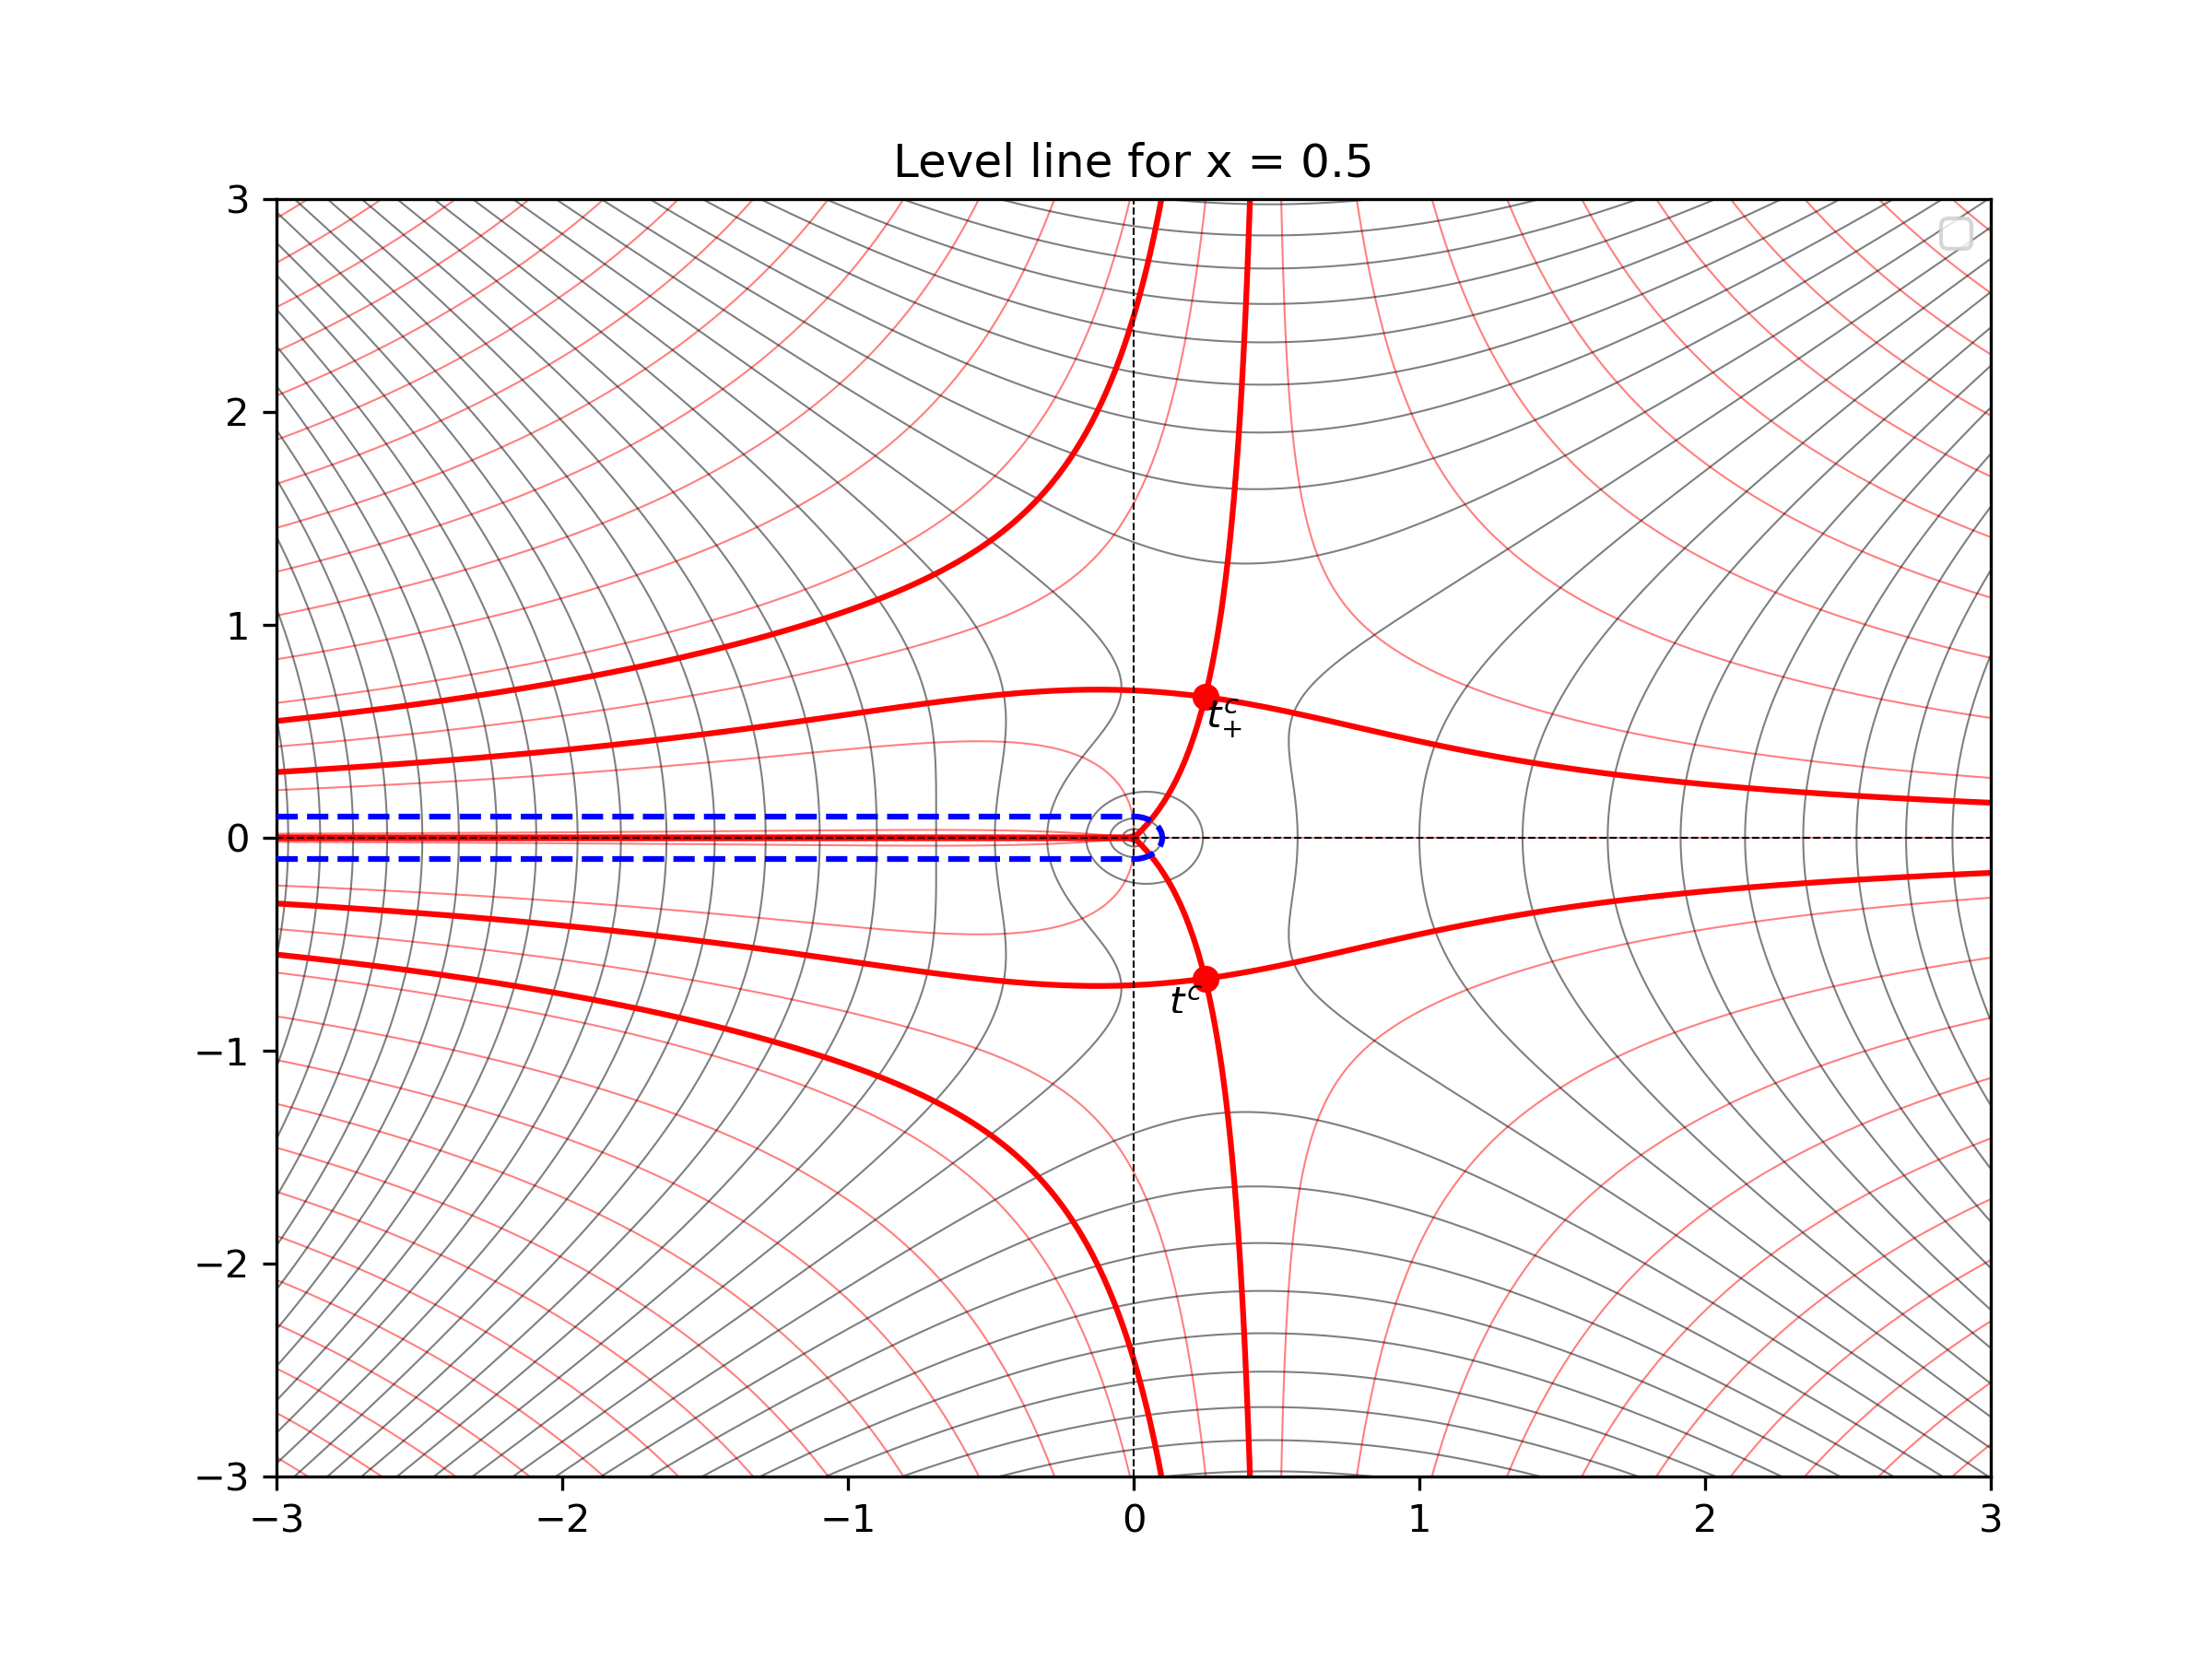
\includegraphics[width=8.5cm]{images/g-contour_plot_theta_0.5.png}
\end{wrapfigure} 

For $-2\sqrt{N} < x < 2\sqrt{N}$, or, equivalently, $-2 < \alpha < 2$ we have, as Figure \ref{wrap-fig:1} suggests, both critical points as complex values, this can also be easily determined noting that if we set $\alpha$ constant with $0 < \alpha < \sqrt{2}$ , we will have
\begin{equation}
	\beta_c^\pm  = \frac{\alpha}{2} \pm \frac{\ii}{2}\sqrt{4 -\alpha^2}.
\end{equation}
And, if we parametrize $\alpha = 2 \cos{(\gamma)}$ for $\gamma \in (0, \pi/2]$ we can rewrite 
\begin{equation}
	\beta_c^\pm = \ee^{\pm \ii \gamma}.
\end{equation}

If we are indeed interested in solving the paths where the imaginary parts are constant, as needed for the Laplace method, we will have to solve an equation such as 
\begin{equation}
	\Im(\phi_{\alpha}(z) - \phi_{\alpha}(\beta_c^\pm)) = 0,
\end{equation} 
for some $z = r \ee^{\ii \theta}$. We first solve for the positive critical point - the negative will be analogous. This equation can be rewritten as a quadratic formulae 
\begin{equation}
	\frac{1}{2} r^2 \sin{(2\theta)} - r \cos{(\gamma)}\sin{(\theta)} + (\theta - \theta_0) = 0
\end{equation} 
where we have set $\theta_0 = \gamma - \frac{1}{2} \sin{(2\gamma)}.$ Where we solve for the two solutions $r_a^+$ and $r_d^-$  by meshing the two quadratic solutions given by the equations. This give us two smooth paths for the positive critical point

\begin{multicols}{2}
	\begin{center}
		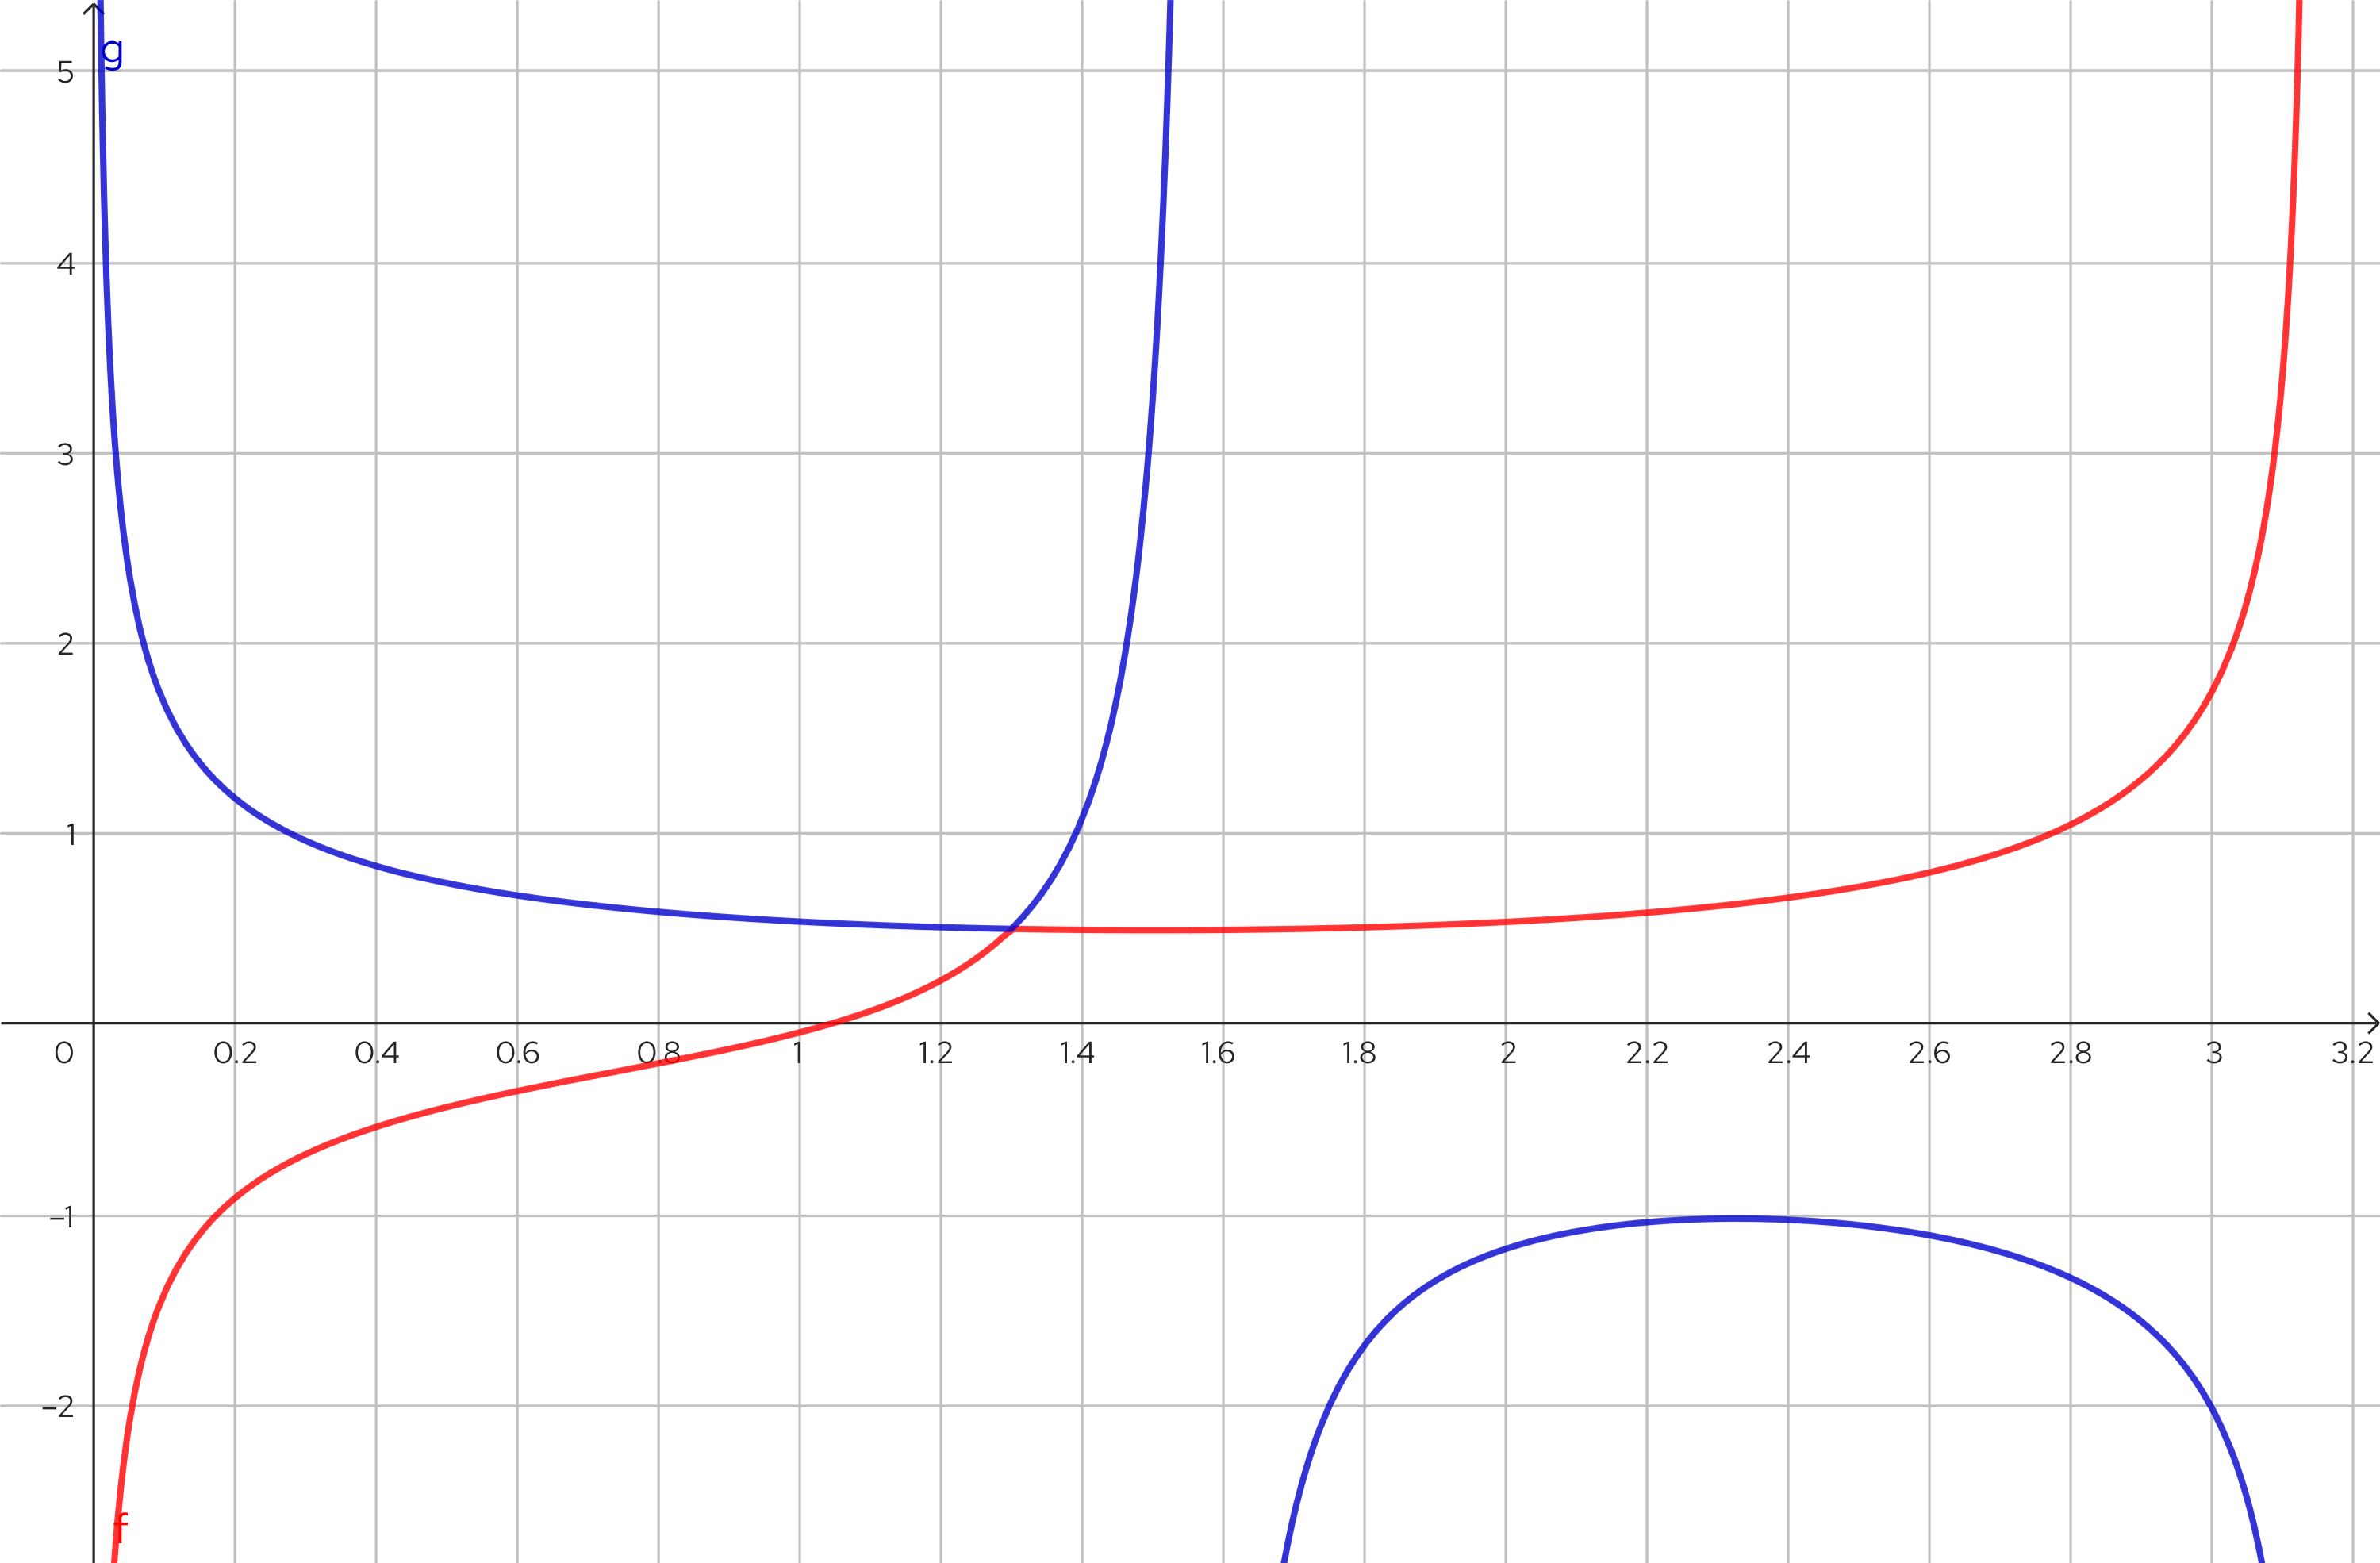
\includegraphics[width=6.5cm]{images/geogebra-export.png}
	\end{center}
	\columnbreak
	\hspace{1cm}
	\begin{equation}
		r_d^+(\theta)  = 
		\begin{cases}
			\frac{\cos{(\gamma)}  - \sqrt{\cos^2{(\gamma)} - (\theta-\theta_0)/\tan{(\theta)}}}{\cos{(\theta)}}; \ \ \theta \in [\gamma, \pi ) \\
			\frac{\cos{(\gamma)}  + \sqrt{\cos^2{(\gamma)} - (\theta-\theta_0)/\tan{(\theta)}}}{\cos{(\theta)}}; \ \ \theta \in (0, \gamma) 
		\end{cases}
	\end{equation}
	\begin{equation}
		r_a^+(\theta) = 
		\begin{cases}
			\frac{\cos{(\gamma)}  + \sqrt{\cos^2{(\gamma)} - (\theta-\theta_0)/\tan{(\theta)}}}{\cos{(\theta)}};  \ \ \theta \in [\gamma, \pi/2 )\\
			\frac{\cos{(\gamma)}  - \sqrt{\cos^2{(\gamma)} - (\theta-\theta_0)/\tan{(\theta)}}}{\cos{(\theta)}}; \ \ \theta \in [\theta_0, \gamma )
		\end{cases}
	\end{equation}
\end{multicols}
With which we can construct both paths of constant imaginary part 
\begin{equation}
	\Gamma_d^+ = \{ r_d^+(\theta) \ee^{\ii \theta} : \theta \in (0, \pi) \}; \ \ \ \Gamma_a^+ = \{ r_a^+(\theta) \ee^{\ii \theta} : \theta \in (0, \pi/2) \}
\end{equation}
%\begin{figure}[h!]
%	\centering
%	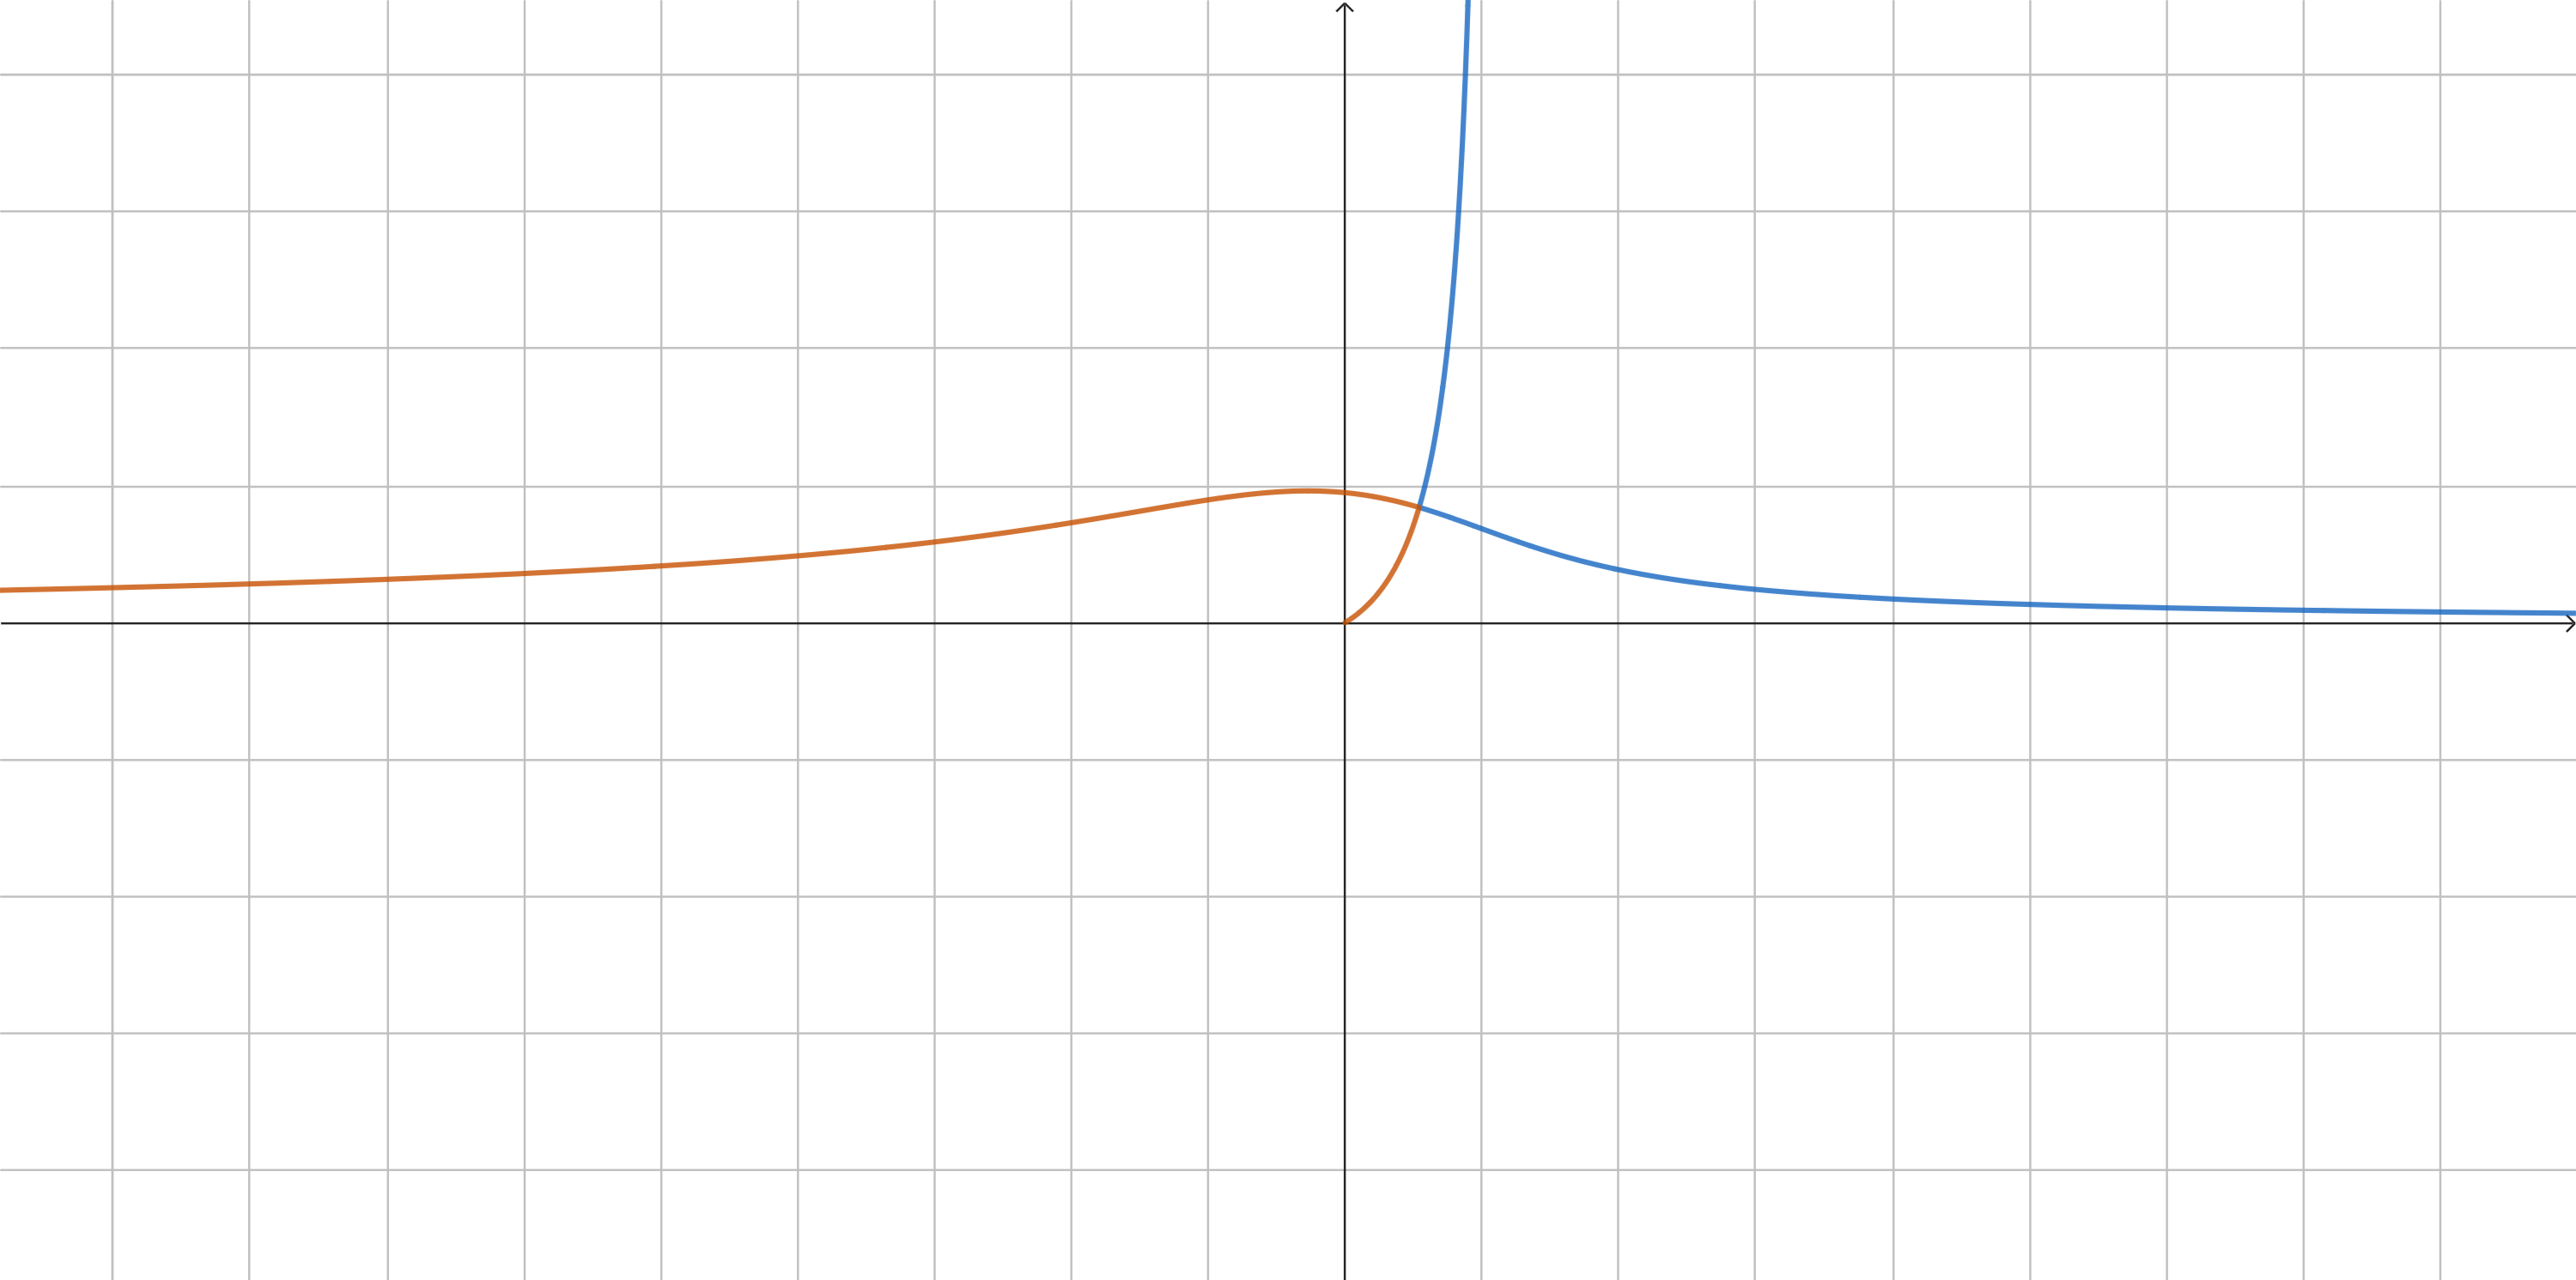
\includegraphics[width=9cm]{images/Hermite1positivepaths.png}
%\end{figure}

Analogously, for the negative part,
\begin{equation}
	\Gamma_d^- = \{ r_d^-(\theta) \ee^{\ii \theta} : \theta \in (0, \pi) \}; \ \ \ \Gamma_a^- = \{ r_a^-(\theta) \ee^{\ii \theta} : \theta \in (0, \pi/2) \}
\end{equation}
%\begin{figure}[h]
%	\centering
%	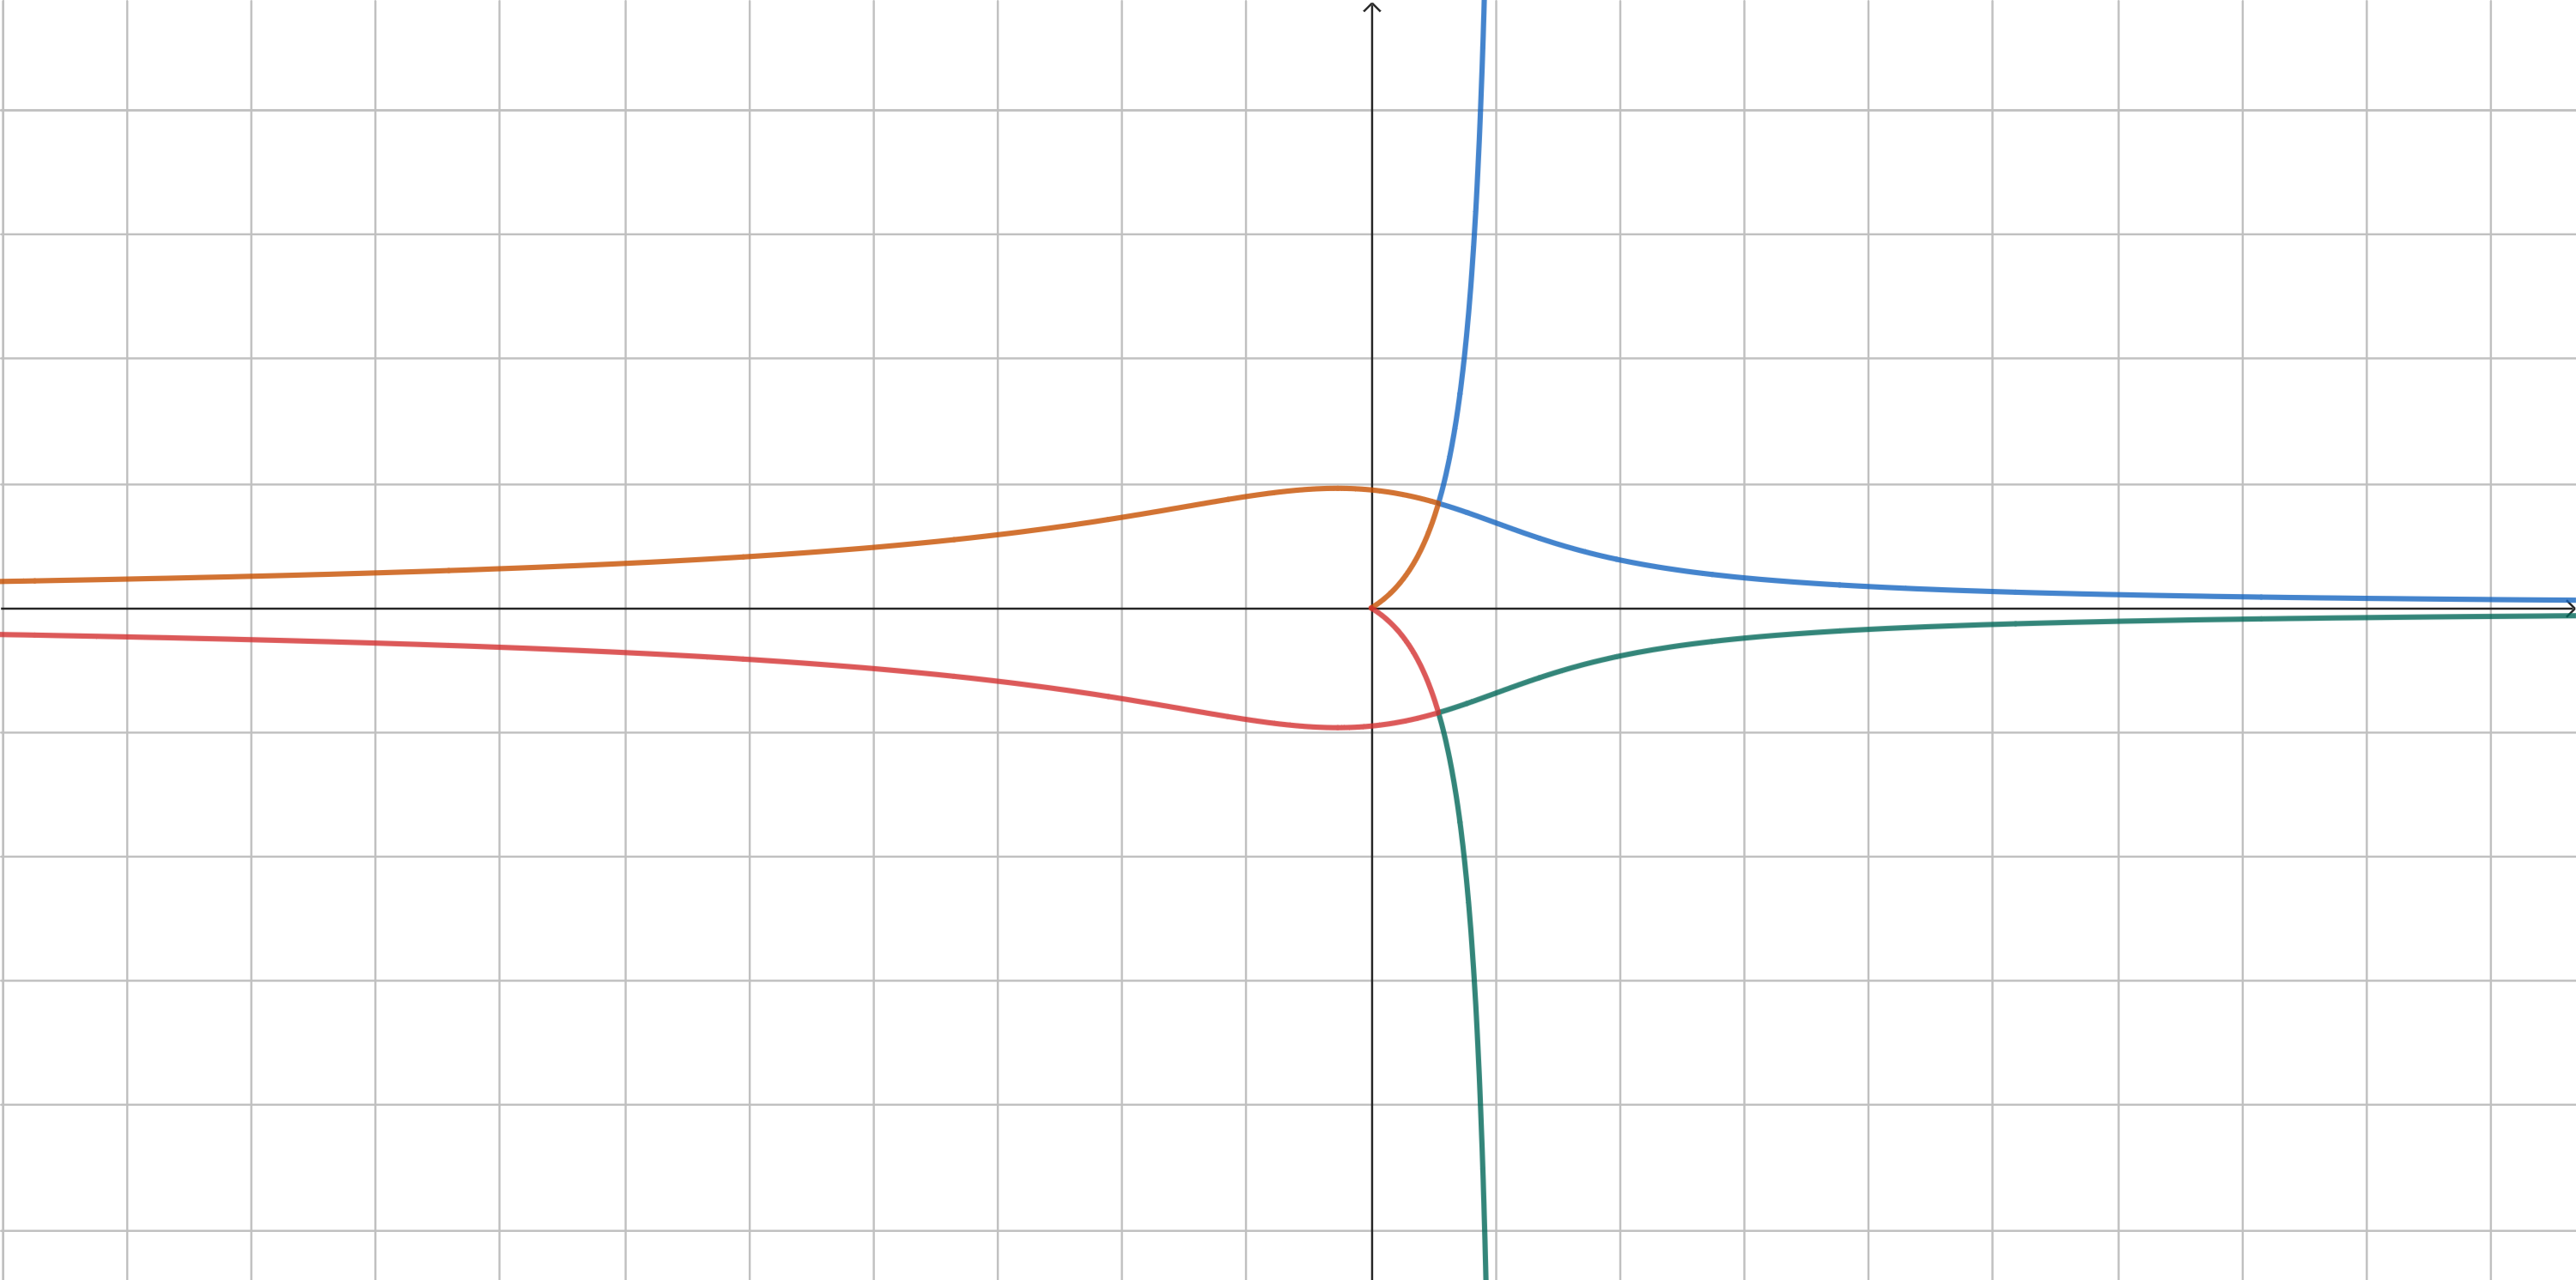
\includegraphics[width=10cm]{images/HermiteCompletePaths.png}
%\end{figure}
Now, we only need to determine the steepest descent path. This should be easy as we know the asymptotic behavior $\phi_\alpha(t) \sim t^2$ for $t \rightarrow \infty$ and that  $\phi_{\alpha}(t) \sim \ln{(t)}$ for $t \rightarrow 0$. From this, follows that $\Gamma_d^+$ and $\Gamma_d^-$ are the paths we were looking for.  We create therefore, a new path $\Gamma_x$ that connects both $\Gamma_d$ at the vertical line $x$. Then, doing $\Gamma \mapsto \Gamma_d^+ \cup \Gamma_d^- \cup \Gamma_x$ and noting that, as $x$ goes to infinity, we have
\begin{equation}
	\left|  \int_{\Gamma_x} g(x) \ee^{-n\phi_\alpha(\beta)} \dd \beta  \right| \leq \max_{y \in \Gamma_x}{\left|  g(x) \ee^{-n\phi_\alpha(\beta)} \right|} \int_{\Gamma_x} |\dd \beta| \stackrel{t \rightarrow \infty}{\rightarrow} 0
\end{equation} 
where $g(t)$ can be both the inverse square root or inverse function. Therefore, we only need to consider the other two paths when considering the asymptotic. Let's briefly discuss how to get the tangent angle of the integration curve.  We know that, locally, we will have $\beta_c^+ + \epsilon \ee^{\ii \theta}$. If we wish to find the angle $\theta$ from which the curve is tangent we must note that this will be the angle in which $\phi_\alpha(\beta_c^+ + \epsilon \ee^{\ii \theta})$ has constant imaginary part - as this is the way th ecurve is defined. Therefore, for some constant $c$,
\begin{align}
	& \Im{\left[ \phi_\alpha(\beta_c^+ + \epsilon \ee^{\ii \theta})\right]} = c \\
	& \implies \Im{\left[ \frac{\phi''(\beta_c)}{2} \ee^{2 \ii \theta}   \right]} =  \sin{\theta} \sin{(2\theta)} = 0, \quad \forall \epsilon \\
	& \implies \theta = k \frac{\pi}{2}, \quad \text{for} \quad k = 1,2,\cdots
\end{align}
Finally, retaking the expression for the Hermite Polynomial,
\begin{equation}
	\begin{split}
		\He_n(2\sqrt{N}\cos(\gamma)) &= C_n^0 \int_{\Gamma}  \ee^{-N \phi_\alpha(\beta)} \dd \beta  = C_n^0  \left[ \int_{\Gamma_d^-}  \ee^{-N \phi_\alpha(\beta)} \dd \beta + \int_{\Gamma_d^+}  \ee^{-N \phi_\alpha(\beta)} \dd \beta  \right]\\
		& \stackrel{(Steepest)}{=}  
		C_n^0 \left(
		\ee^{-N(\phi_\alpha(\beta_c^+))} 
		\left[
		\frac{\sqrt{2\pi}}{N^{\frac{1}{2}}}
		\frac{\ee^{\ii (\theta(\beta_c^+))}}{\sqrt{2\sin{(\gamma)}}} 
		+ \Boh(N^{-\frac{3}{2}})
		\right]
		+
		\ee^{-N(\overline{\phi_\alpha(\beta_c^+)})} 
		\left[
		\frac{\sqrt{2\pi}}{N^{\frac{1}{2}}}
		\frac{\ee^{\ii (\overline{\theta(\beta_c^+)})}}{\sqrt{2\sin{(\gamma)}}}
		+ \Boh(N^{-\frac{3}{2}})
		\right]   
		\right)
		\\
		& = C_n^0 \sqrt{\frac{2\pi}{2N\sin{(\gamma)}}} \left(
		\ee^{-N(\phi_\alpha(\beta_c^+))} 
		\left[
		\ee^{\ii(\theta(\beta_c^+))} 
		+ \Boh(N^{-1})
		\right]
		+
		\ee^{-N(\overline{\phi_\alpha(\beta_c^+)})} 
		\left[
		\ee^{\ii(\overline{\theta(\beta_c^+)})}
		+ \Boh(N^{-1})
		\right]   
		\right)
		\\
		& = C_n^0 \sqrt{\frac{\pi}{N\sin{(\gamma)}}}
		\left(
		\ee^{-N(\phi_\alpha(\beta_c^+)) + \ii(\theta(\beta_c^+))} +
		\ee^{-N(\overline{\phi_\alpha(\beta_c^+)})+\ii(\overline{\theta(\beta_c^+)})} 
		\right)
		(1 + \Boh(N^{-1}))   
		\\
		& =  C_n^0 \sqrt{\frac{\pi}{N\sin{(\gamma)}}}
		\left(
		\ee^{-\ii\theta(\beta_c^+) - N (-\alpha \beta_c^+ + \frac{1}{2} (\beta_c^+)^2 + \ln{(\beta_c^+)}) }
		+
		\ee^{\ii \pi} \ee^{\ii\theta(\beta_c^+) - N \overline{(-\alpha \beta_c^+ + \frac{1}{2} (\beta_c^+)^2 + \ln{(\beta_c^+)}) }}  
		\right)
		(1 + \Boh(N^{-1})) 
		\\
		& =  C_n^0 \sqrt{\frac{\pi}{N\sin{(\gamma)}}} \ee^{N(\cos^2{(\gamma)} + \frac{1}{2})}
		\left(
		\ee^{-\ii \left(-N\left(\frac{\sin{(2\gamma)}}{2}-\gamma\right)+ \theta(\beta_c^+)
			\right)}
		-
		\ee^{\ii
			\left(-N\left(\frac{\sin{(2\gamma)}}{2}-\gamma\right)+\theta(\beta_c^+)
			\right)}  
		\right)
		(1 + \Boh(N^{-1})) 
		\\
		& =  C_n^0 \sqrt{\frac{\pi}{N\sin{(\gamma)}}} \ee^{N(\cos^2{(\gamma)} + \frac{1}{2})}
		2\ii \sin{\left(\theta(\beta_c^+)-N\left(\frac{\sin{(2\gamma)}}{2}-\gamma\right)\right)} 
		(1 + \Boh(N^{-1})) \\
		& = \frac{(N-1)! N^{\frac{1}{2}\left(1-N\right)}}{2\pi \ii} \sqrt{\frac{\pi}{N\sin{(\gamma)}}} \ee^{N(\cos^2{(\gamma)} + \frac{1}{2})}
		2\ii \sin{
			\left(
			\theta(\beta_c^+)
			-N\left(\frac{\sin{(2\gamma)}}{2}-\gamma\right)
			\right)} 
		(1 + \Boh(N^{-1})) \\
		%		 & = \sqrt{\frac{2}{\sin{(\gamma)}}} N^{-\frac{N}{2}} (N-1)^{\left(N - \frac{1}{2}\right)} \ee^{N\left(-\cos^2{(\gamma)} + \frac{1}{2} \right) + 1} \sin{\left(\theta(\beta_c^+) -N\left(\frac{\sin{(2\gamma)}}{2}-\gamma\right)
			%		 \right)} 
		%		 (1 + \Boh(N^{-1})) \\
		& = \sqrt{\frac{2}{\sin{(\gamma)}}}
		N^{\frac{1}{2} \left(N - 1\right)}
		\ee^{N\left(\cos^2{(\gamma)} - \frac{1}{2} \right)} 
		\sin{
			\left(
			\theta(\beta_c^+) 
			-N\left(\frac{\sin{(2\gamma)}}{2}
			-\gamma\right)
			\right)
		} 
		(1 + \Boh(N^{-1}))
	\end{split}
\end{equation}
Where we used Stirling's Formula and the fact that we have
\begin{equation}
	\begin{cases}
		\Re[(-\alpha \beta_c^+ + \frac{1}{2} (\beta_c^+)^2 + \ln{(\beta_c^+)})] = -\cos^2{(\gamma)} - \frac{1}{2}; \qquad \Im[(-\alpha \beta_c^+ + \frac{1}{2} (\beta_c^+)^2 + \ln{(\beta_c^+)})] = -\frac{\sin{(2\gamma)}}{2} + \gamma; \\
		\Re[ \overline{(-\alpha \beta_c^+ + \frac{1}{2} (\beta_c^+)^2 + \ln{(\beta_c^+)})} ] = -\cos^2{(\gamma)} - \frac{1}{2}; \qquad  \Im[ \overline{(-\alpha \beta_c^+ + \frac{1}{2} (\beta_c^+)^2 + \ln{(\beta_c^+)})}] = \frac{\sin{(2\gamma)}}{2} - \gamma.
	\end{cases}
\end{equation}
and 
\begin{align}
	(N-k)^{(aN - b)} & = N^{aN - b} \left(1 - \frac{k}{N} \right)^{aN - b} = N^{aN - b} \left(1 - \frac{k}{N} \right)^{aN} \left(1 - \frac{k}{N} \right)^{-b} \\
	& = N^{aN - b} \ee^{aN \ln{\left(1 - \frac{k}{N} \right)}}  \left(1 + \Boh(N^{-1}) \right) \\
	& = N^{aN - b} \ee^{aN (-\frac{k}{N} + \Boh{(N^{-2})})}  \left(1 + \Boh(N^{-1}) \right) \\
	& = N^{aN - b} \ee^{-ak}  \left(1 + \Boh(N^{-1}) \right)
	\label{Equation: Approximation for N powers}
\end{align}
Of course, if we change for the other case we can simply rewrite
\begin{equation}
	\He_{n-1}(2\sqrt{N}\cos(\gamma)) = \sqrt{\frac{2}{\sin{(\gamma)}}}
	N^{\frac{1}{2} \left(N -2\right)}
	\frac{\ee^{N\left(\cos^2{(\gamma)} - \frac{1}{2} \right)}}{\ee^{\cos^2{(\gamma)}}}
	\sin{
		\left(
		\theta(\beta_c^+) 
		-(N-1)\left(\frac{\sin{(2\gamma)}}{2}
		-\gamma\right)
		\right)
	} 
	(1 + \Boh(N^{-1}))
\end{equation}

\textbf{Case 2}

\begin{wrapfigure}{H}{8.5cm}
	\caption{Figure for case 3}\label{wrap-fig:2}
	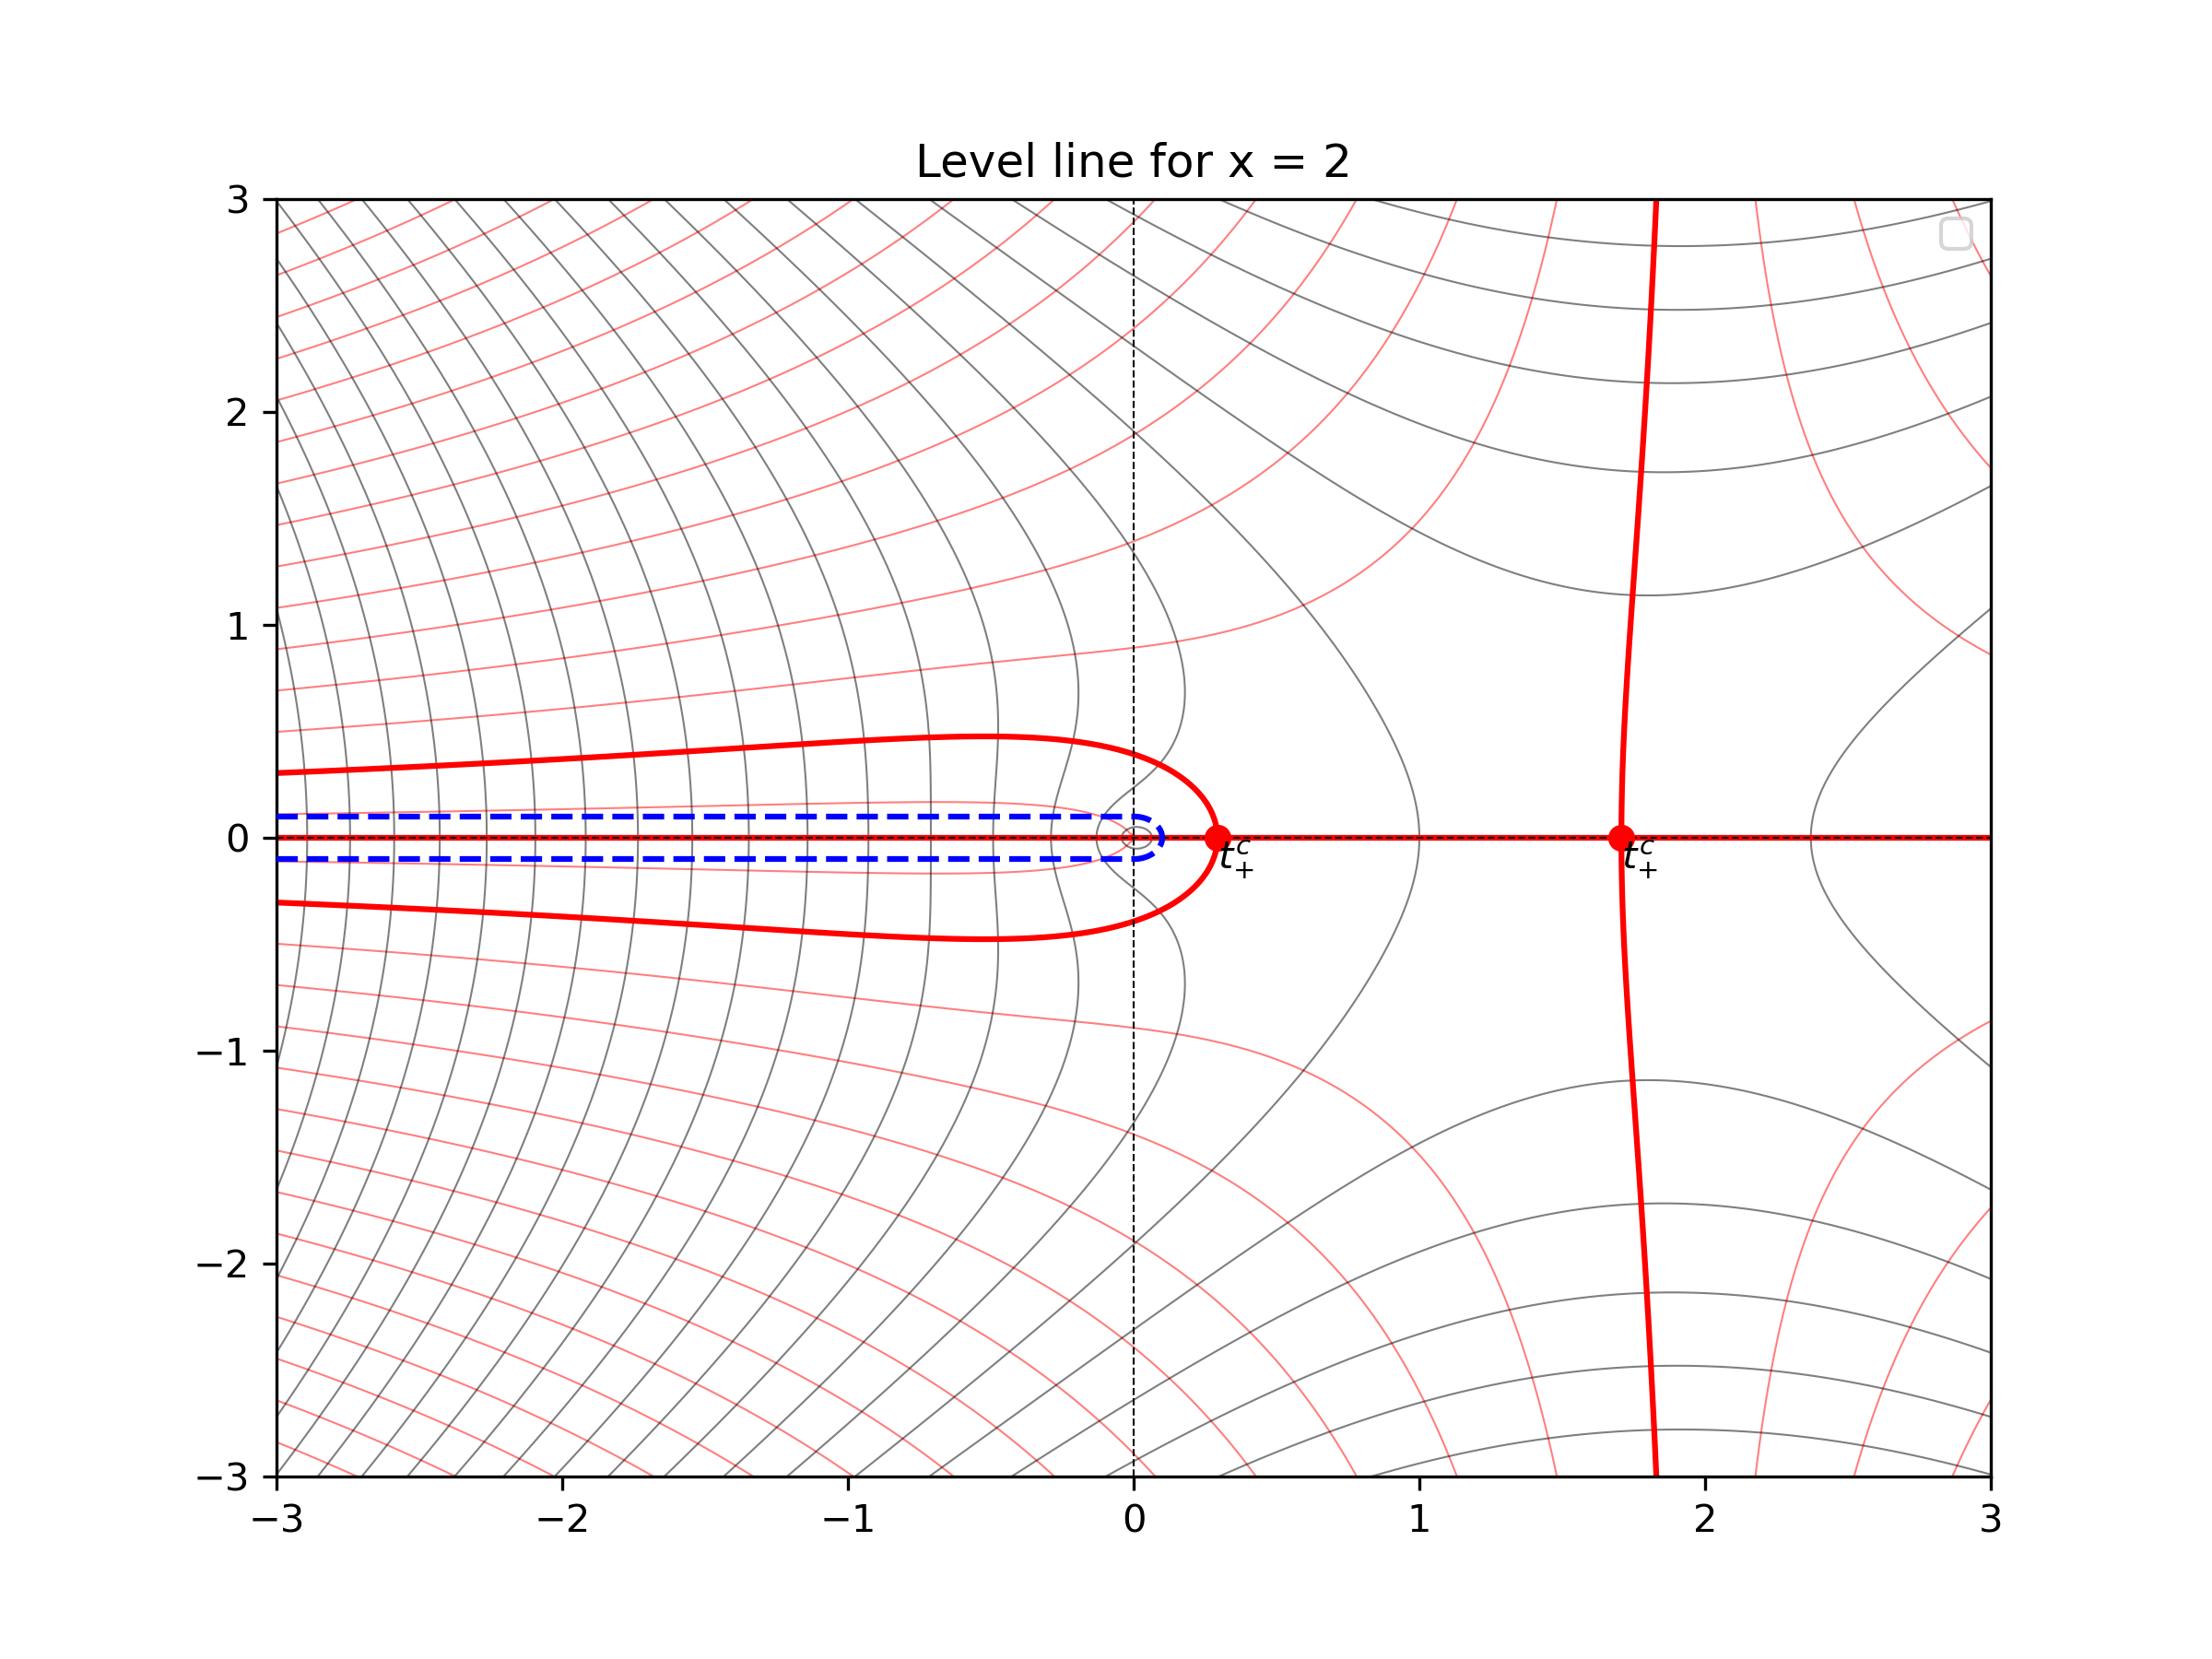
\includegraphics[width=8.5cm]{images/g-contour_plot_theta_2.png}
\end{wrapfigure} 

Here, with $|x| > 2\sqrt{N}$, or equivalently $ \alpha > 2$,  we have - as the plot \ref{wrap-fig:2} suggests - both critical points as real values, this can be easily determined noting that if we set $\alpha > 2$ , we will have
\begin{equation}
	\beta_c^\pm  = \frac{\alpha}{2} \pm \frac{1}{2}\sqrt{\alpha^2 - 4}.
\end{equation}
And, if we parametrize $\alpha = 2 \cosh{(\gamma)}$ for $\gamma > 1$ we can rewrite 
\begin{equation}
	\beta_c^\pm = \ee^{\pm \gamma}.
\end{equation}
If we are indeed interested in solving the paths where the imaginary parts are constant, as needed for the Laplace method, we will have to sove an equation such as 
\begin{equation}
	\Im(\phi_{\alpha}(z) - \phi_{\alpha}(\beta_c^\pm)) = 0,
\end{equation} 
for some $z = r \ee^{\ii \theta}$. We first solve for the positive critical point and he negative will be analogous. This can be rewritten as  as quadratic equation 
\begin{equation}
	\frac{1}{2}r^2 \sin{(2\theta)} - r \cosh{(\gamma)}\sin{(\theta)} + \theta = 0
\end{equation}
where we solve for the two solutions $r_a^+$ and $r_d^-$  by meshing the two quadratic solutions given by the equations. This give us two smooth paths for the positive critical point

\begin{multicols}{2}
	\begin{center}
		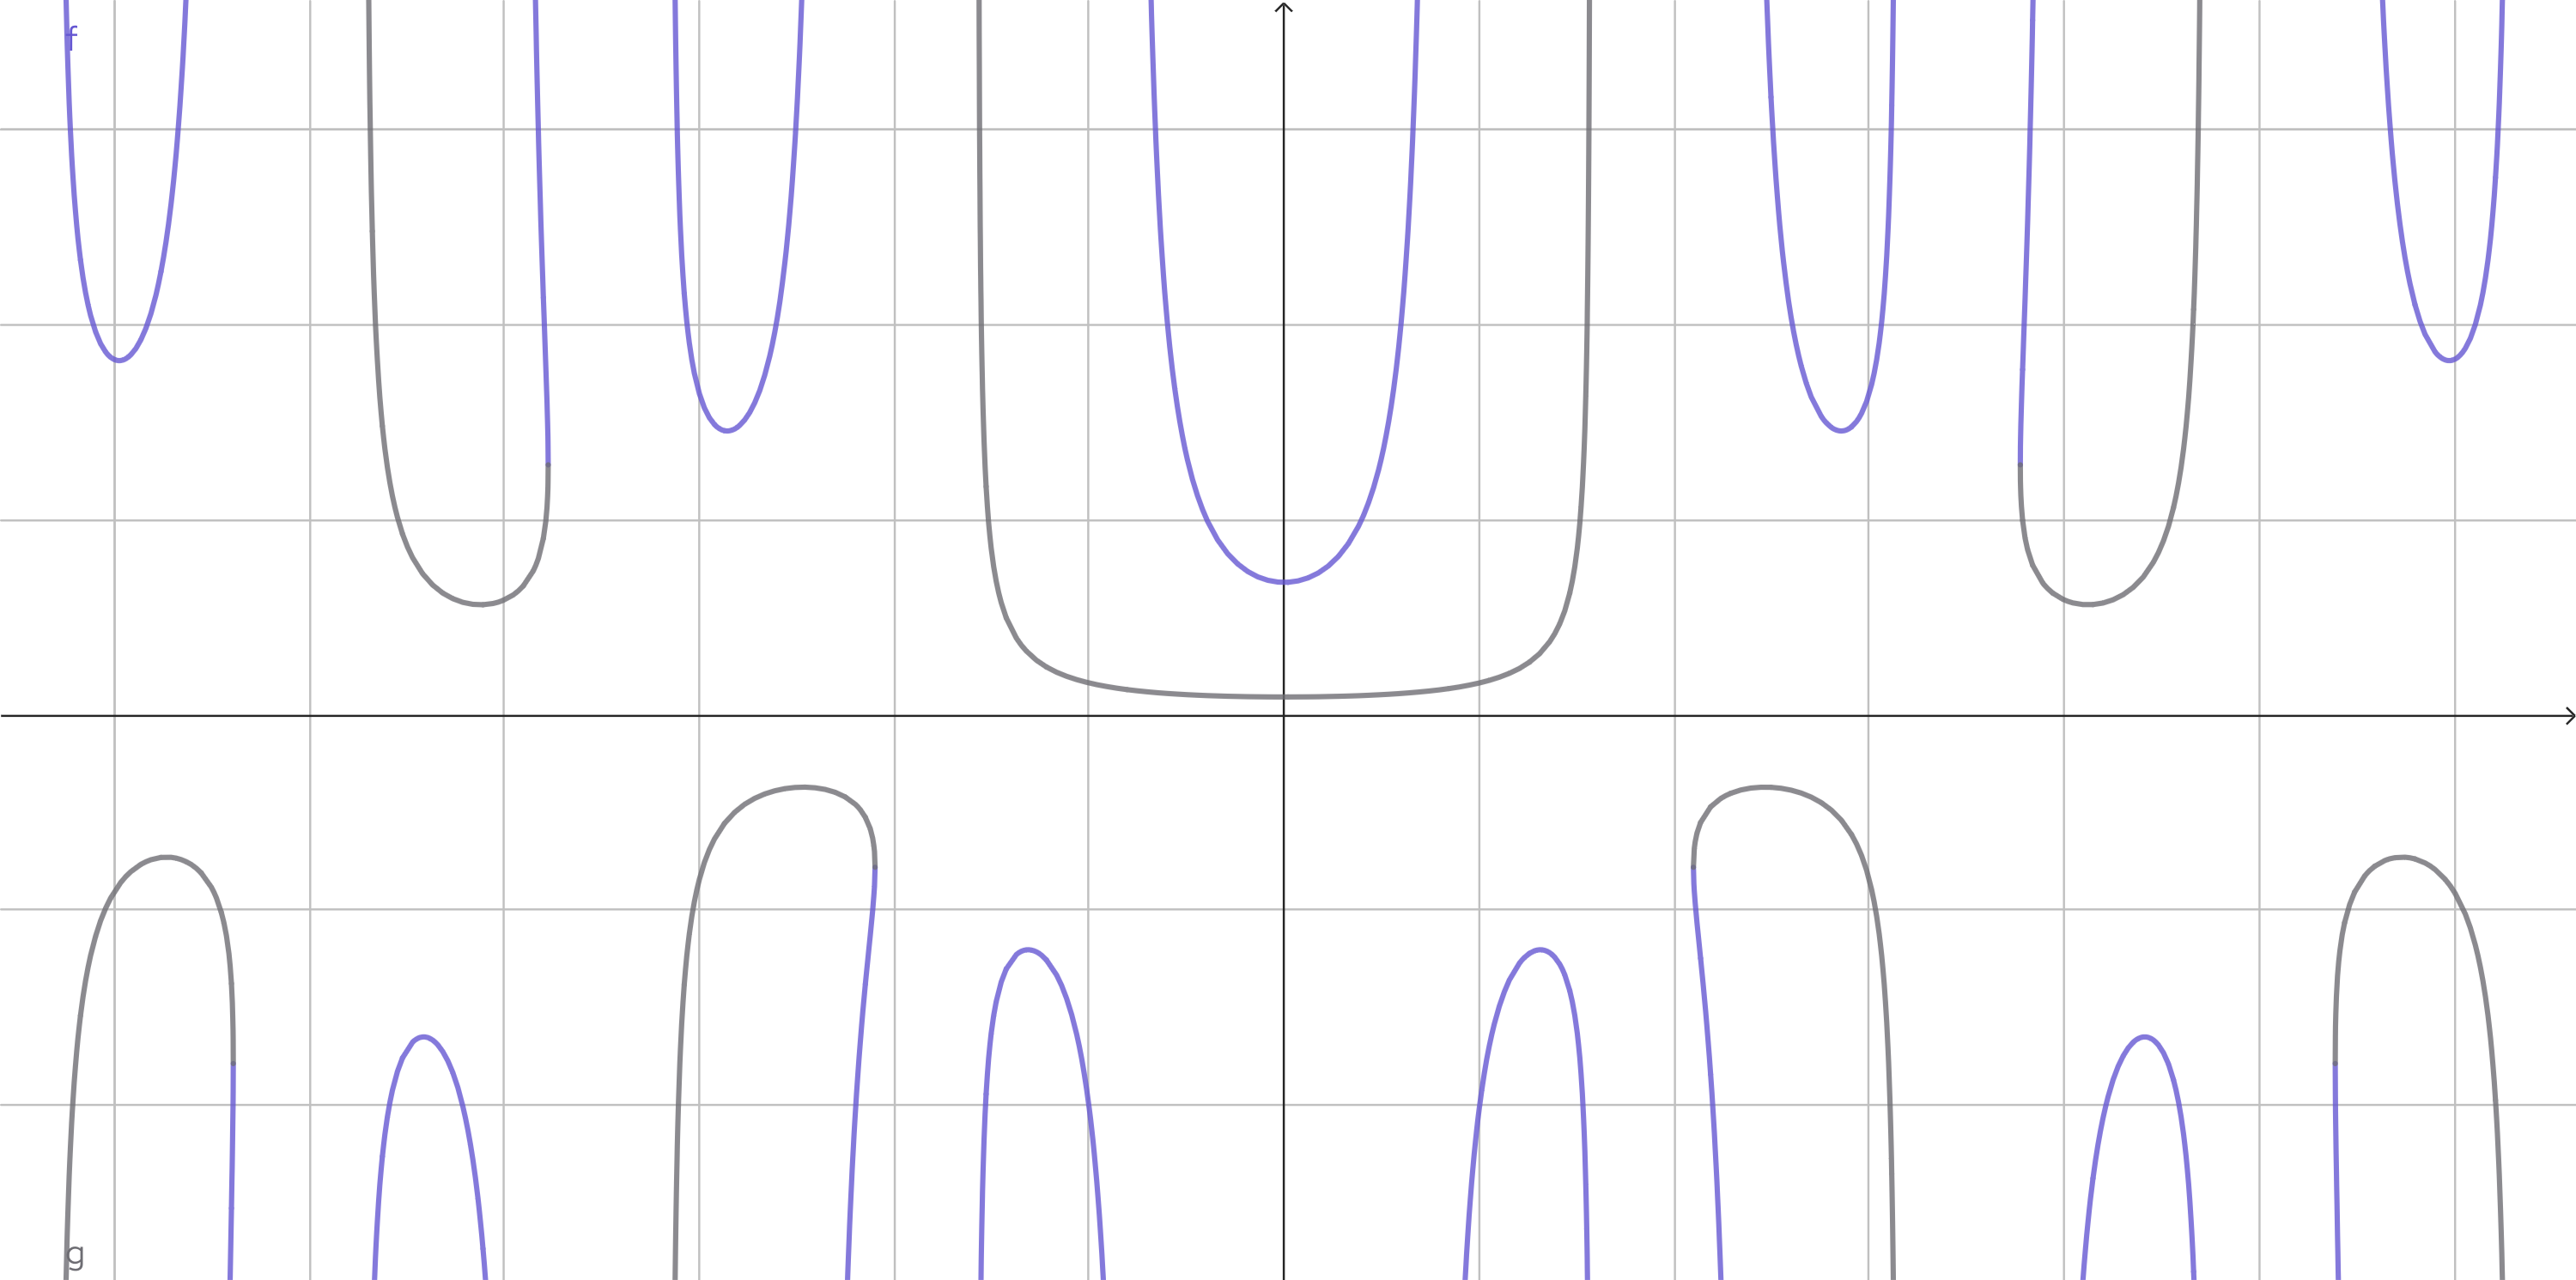
\includegraphics[width=7cm]{images/HermiteCase2Positive.png}
	\end{center}
	\columnbreak
	\hspace{0.2cm}
	\begin{equation}
		r_d(\theta)  = \frac{\cosh{(\gamma)}  - \sqrt{\cosh^2{(\gamma)} - \frac{\cosh{(\gamma)} \theta}{\sin{(\theta)}}}}{\cos{(\theta)}}; \ \ \theta \in [0, \pi )
	\end{equation}
	\begin{equation}
		r_a(\theta)  = \frac{\cosh{(\gamma)}  + \sqrt{\cosh^2{(\gamma)} - \frac{\cosh{(\gamma)} \theta}{\sin{(\theta)}}}}{\cos{(\theta)}}; \ \ \theta \in [0, \pi )
	\end{equation}
\end{multicols}

With which we can construct both paths of constant imaginary part 
\begin{equation}
	\Gamma_d = \{ \tilde{r}_d(\theta) \ee^{\ii \theta} : \theta \in (0, 2\pi) \}; \ \ \ \Gamma_a = \{ \tilde{r}_a(\theta) \ee^{\ii \theta} : \theta \in (0, 2\pi) \} 
\end{equation}

%\begin{figure}[h]
%	\centering
%	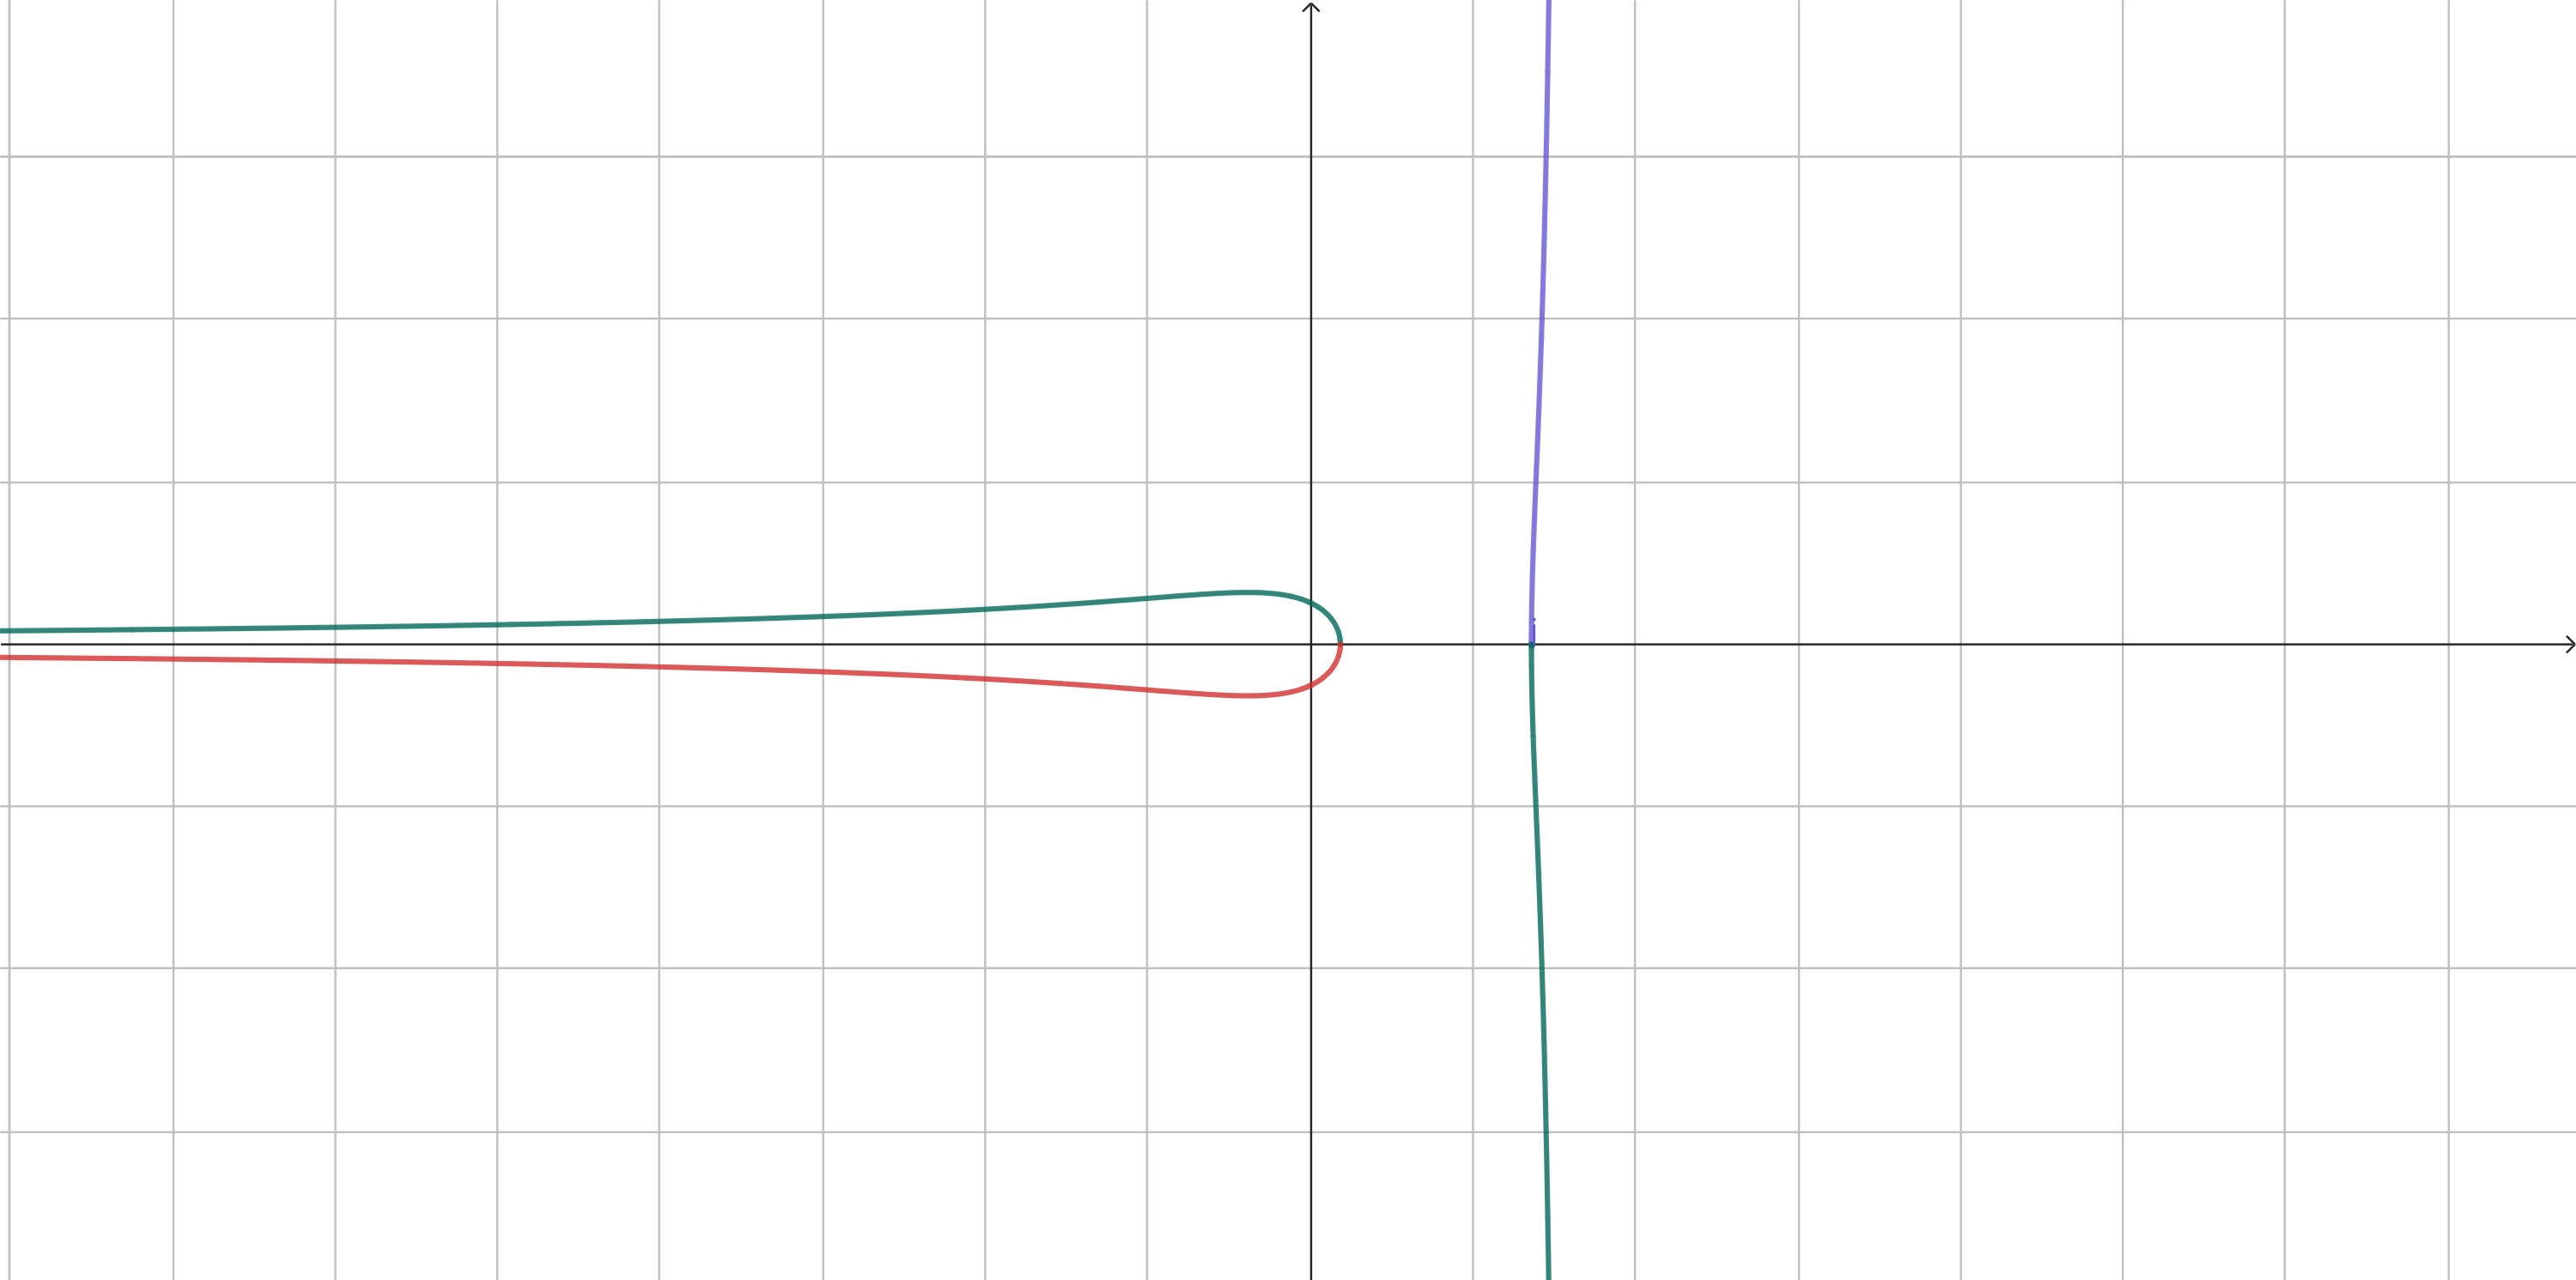
\includegraphics[width=10cm]{images/HermiteCase2PathsPositive.png}
%\end{figure}

We need now to determine the Steepest Descent Path. In this case is more clear what the path should be the one passing through the critical point $\ee^{-\gamma}$.  An argument of symmetry allow us to show that the tangent angle of the path of steepest descent must be $2\pi/4$, as the curve - together with the real line - divide the plane into 4 parts. Then, repeating the process we did on Case 1 - changing the path of integration - we can make the substitution
\begin{align}
	\He_{n}(2\sqrt{N}\cosh{(\gamma)}) &= C_n^0 \int_{\Gamma}  \ee^{-N \phi_\alpha(\beta)} \dd \beta \\
	&= C_n^0 \int_{\Gamma_d}  \ee^{-N \phi_\alpha(\beta)} \dd \beta \\
	& \stackrel{(Steepest)}{=}  C_n^0  \ee^{N(\phi_\alpha(\beta_c^-))} 
	\left[
	\frac{\sqrt{2\pi}}{N^{\frac{1}{2}}}
	\frac{\ee^{\ii (\theta(\beta_c^-))}}{\sqrt{|1 - \ee^{2\gamma}|}} 
	+ \Boh(N^{-\frac{3}{2}})
	\right]
	\\
	&= C_n^0  
	\ee^{-N(\phi_\alpha(\beta_c^-))}
	\frac{\sqrt{2\pi}}{N^{\frac{1}{2}}}
	\frac{\ee^{\ii (\theta(\beta_c^-))}}{\sqrt{|1 - \ee^{2\gamma}|}} 
	\left(1 + \Boh(N^{-1}) \right)
	\\
	&= 	\ee^{-N(\phi_\alpha(\beta_c^-))} \frac{(N-1)! N^{\frac{1}{2}\left(1-N\right)}}{2\pi \ii} 
	\frac{\sqrt{2\pi}}{N^{\frac{1}{2}}}
	\frac{\ii}{\sqrt{|1 - \ee^{2\gamma}|}} 
	\left(1 + \Boh(N^{-1}) \right)
	\\
	&= 	\ee^{-N(\phi_\alpha(\beta_c^-) - 1) + 1} \frac{(N-1)^{N - \frac{1}{2}} N^{-\frac{N}{2}}}{\sqrt{|1 - \ee^{2\gamma}|}} 
	\left(1 + \Boh(N^{-1}) \right)
	\\
	& =	\ee^{-N( \phi_\alpha(\beta_c^-) - 1) + 1} \frac{(N-1)^{N - \frac{1}{2}} N^{-\frac{N}{2}}}{\sqrt{|1 - \ee^{2\gamma}|}} 
	\left(1 + \Boh(N^{-1}) \right) \\
	& =	\ee^{-N\left( \frac{\ee^{-2\gamma}}{2} + \gamma +  1\right) + 1} \frac{(N-1)^{N - \frac{1}{2}} N^{-\frac{N}{2}}}{\sqrt{|1 - \ee^{2\gamma}|}} 
	\left(1 + \Boh(N^{-1}) \right) \\
	& =	\ee^{-N\left( \frac{\ee^{-2\gamma}}{2} + \gamma +  1\right)} \frac{N^{\frac{1}{2}\left(N - 1\right)}}{\sqrt{|1 - \ee^{2\gamma}|}} 
	\left(1 + \Boh(N^{-1}) \right)
\end{align}
Similarly, for the other case
\begin{equation}
	\He_{n-1}(2\sqrt{N}\cosh{(\gamma)}) = \frac{\ee^{-N\left( \frac{\ee^{-2\gamma}}{2} + \gamma +  1\right)}}{\ee^{\left( \frac{\ee^{-2\gamma}}{2} + \gamma + \frac{3}{2}\right)}} \frac{N^{\frac{1}{2}\left(N -2\right)}}{\sqrt{|1 - \ee^{2\gamma}|}} 
	\left(1 + \Boh(N^{-1}) \right)
\end{equation}


\textbf{Case 3}

\begin{wrapfigure}{h!}{8.5cm}
	\caption{Figure for case 3}\label{wrap-fig:3}
	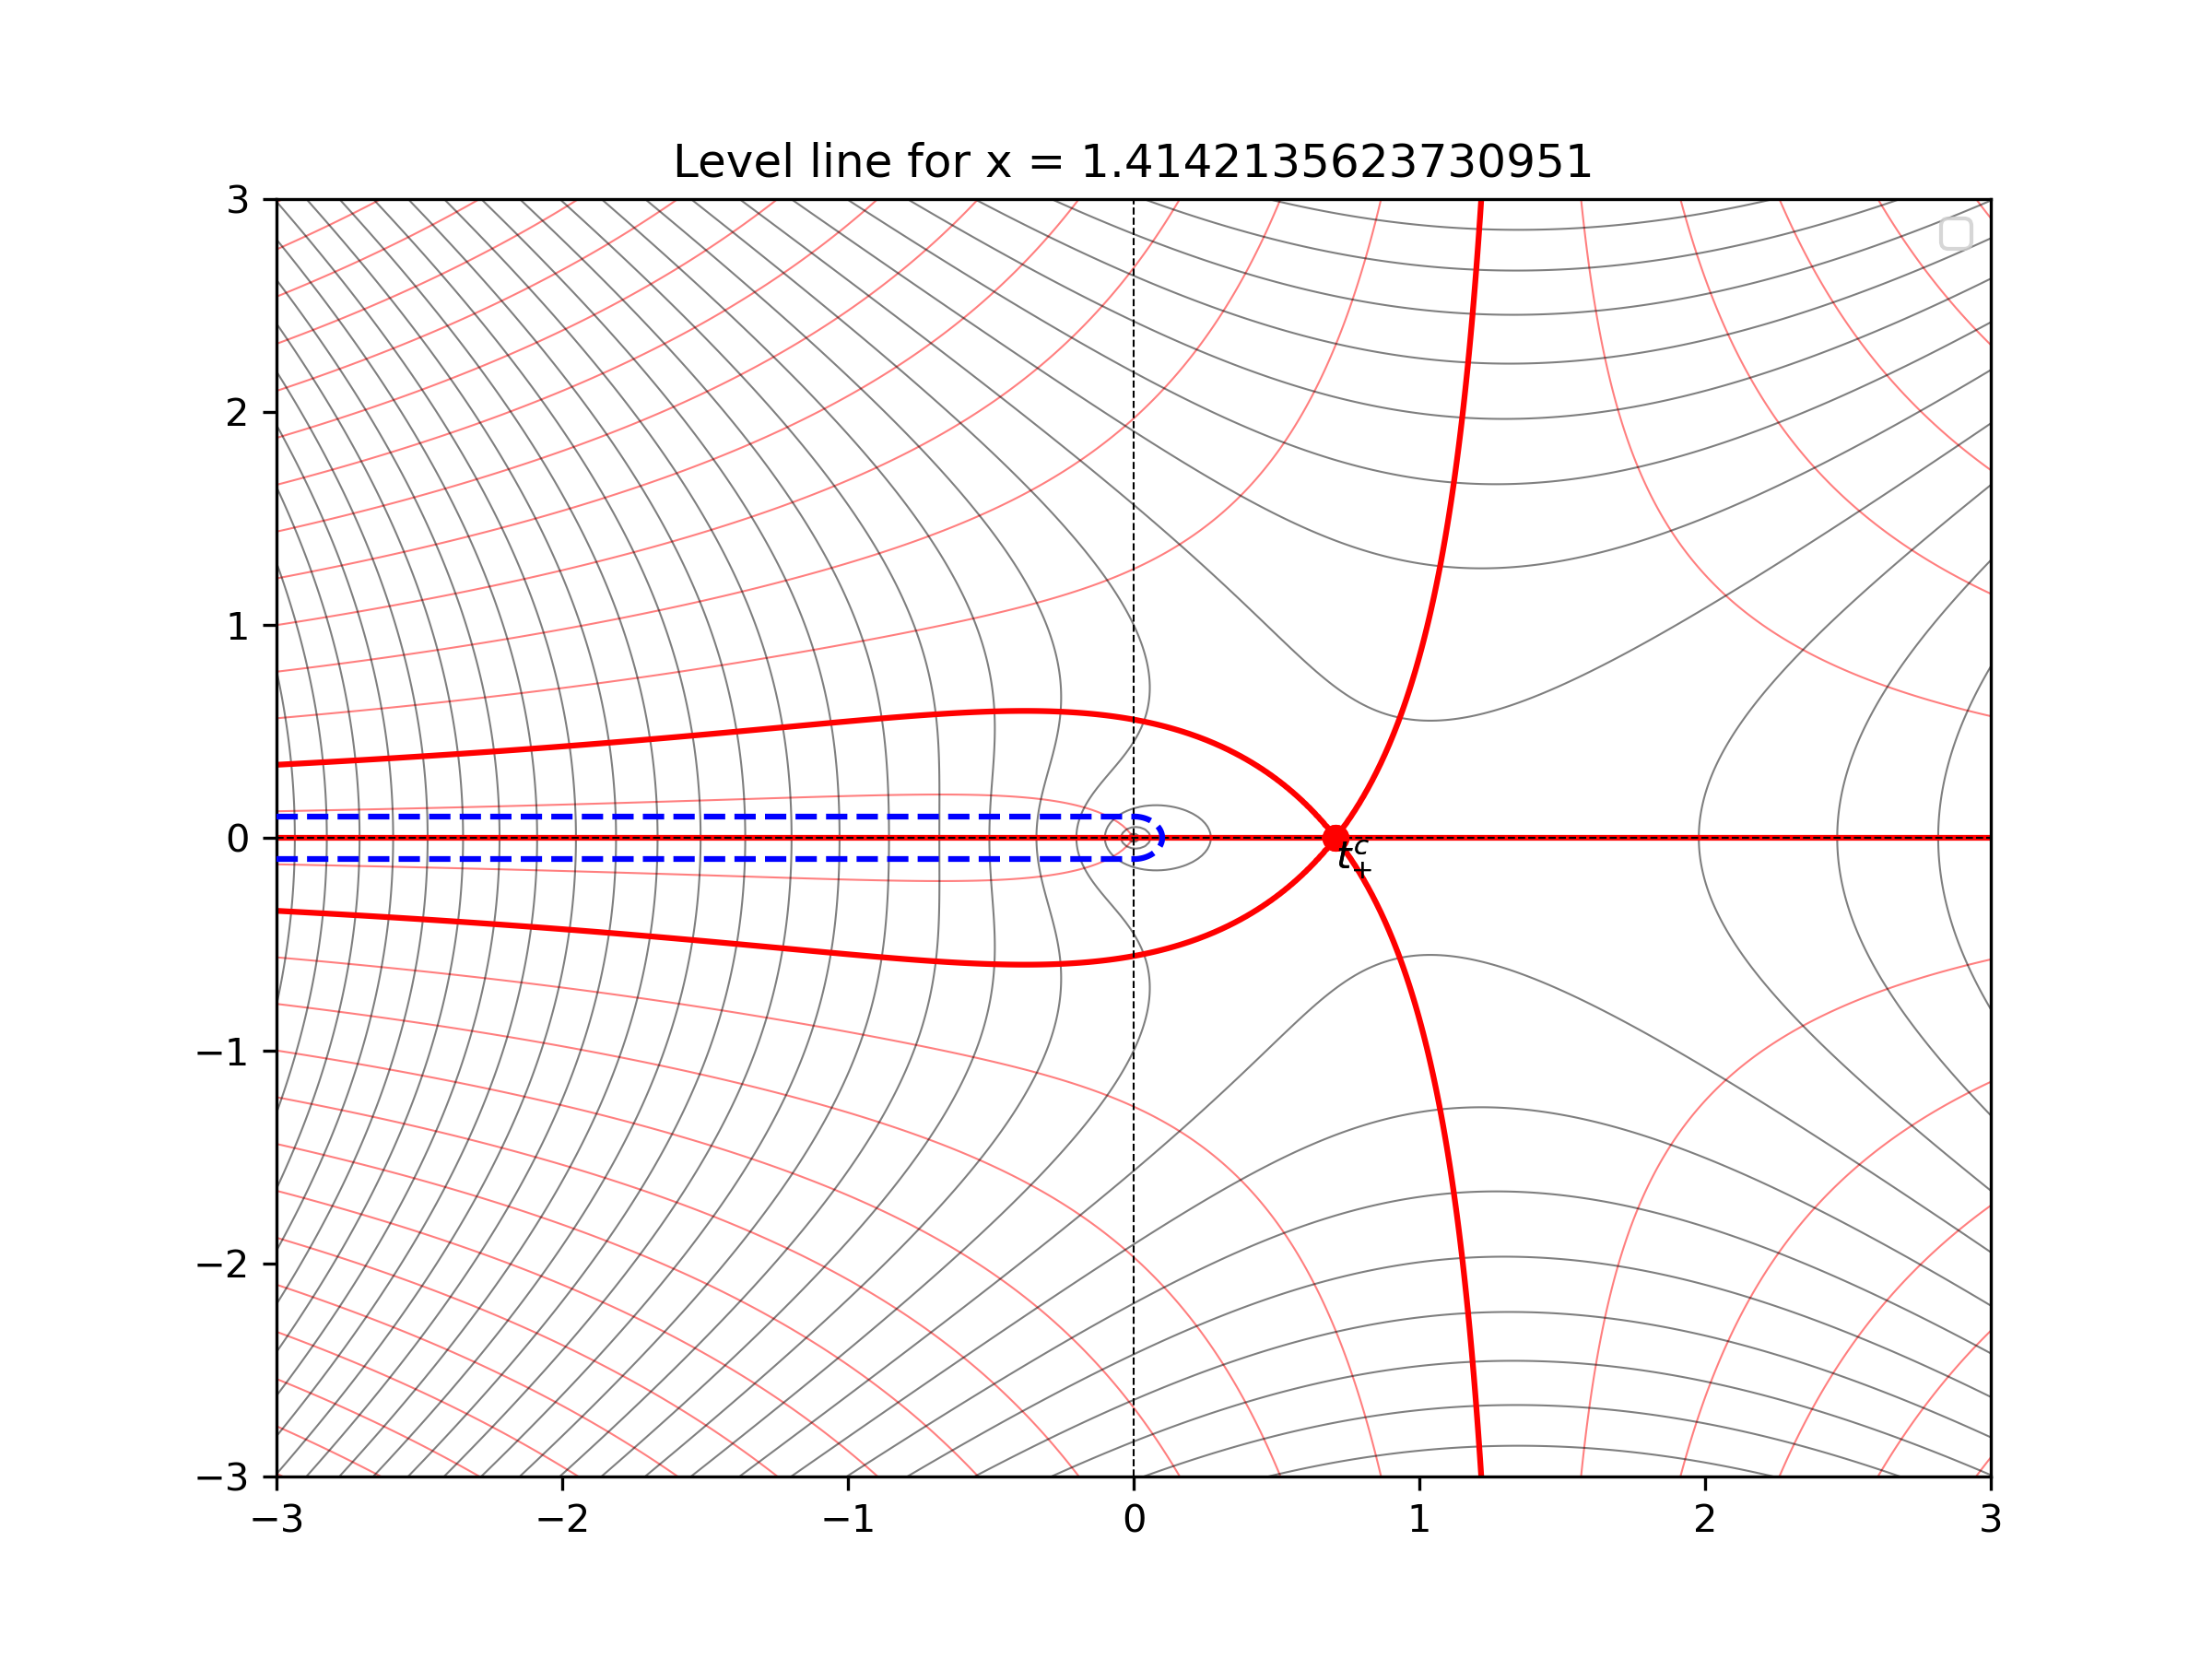
\includegraphics[width=8.5cm]{images/g-contour_plot_theta_1.4.png}
\end{wrapfigure} 

%Take the Definition \ref{Def: Airy Function} for the Airy Function. Take $\langle$ to be the union of the lines  $\{t\ee^{\ii 2\pi/6} : t \geq 0\}$ and $\{ t\ee^{-\ii 2\pi/6}: t \geq 0\}$. Applying the change of variables $t=-\ii z$ - which rotates the integration contour $\wedge$ into $\langle$, with $\dd w = - \frac{\dd t}{\ii}$ and $z^3 = t^3$, we see that the Airy Function can be written
%\begin{equation}
%	\Ai(u) = \frac{1}{2\pi} \int_{\rangle} \exp{\left( \frac{\ii}{3} z^3 + \ii u z \right)} \dd z
%\end{equation} 

Let's start with a sketch of the proof for this behavior.
\begin{enumerate}
	\item \textbf{Step One}: Write the integral for $N = n + 1$
	\begin{equation}
		\He_n(\sqrt{N}\alpha) = C_n^0 \int_{\Gamma}  \ee^{-N \phi_\alpha(\beta) } \dd \beta
	\end{equation} 
	where $\phi_\alpha(\beta) = \beta^2 -2 \alpha \beta + \ln{(\beta)}$;
	\item \textbf{Step two}: The function $\phi_{\alpha}(\beta)$ has a double critical point at $2$. The steepest descent curve is defined by $\Im(\phi_{\alpha}(z) - \phi_{\alpha}(2)) = 0$;
	\item \textbf{Step three}: Deform the contour such that the only contribution for the integral comes from the critical point . Computing the Taylor approximation to the third order we have
	\begin{equation}
		\phi_{\alpha}(\beta) = \phi_\alpha(\sqrt{2}/2) + \phi^{(3)}_\alpha(\sqrt{2}/2) (\beta - \beta_c)^3 + \Boh(\beta^4)  
	\end{equation}
	and perform the change fo variables $\lambda = N^{\frac{1}{3}}(\beta-\beta_c)$ to obtain
	\begin{equation}
		\He_n(\sqrt{N}\alpha) \approx \tilde{C_n} \int_{\Gamma}  \ee^{\lambda^3} \dd \lambda
	\end{equation} 
	\item \textbf{Step four} Recognize the Airy Function and write
	\begin{equation}
		\He_n(\sqrt{N}\alpha) \propto \Ai(0)
	\end{equation}
\end{enumerate}

We start with the expression determined in \eqref{Equation: Hermite Integral}, working on the edge, we will set $x = 2\sqrt{N} + \xi N^{-\frac{1}{6}}$, that is, $\alpha = 2 + \xi N^{-\frac{2}{3}}$. Remember the expression
\begin{equation}
	\He_n(\sqrt{N}\alpha) = C_n^0 \int_{\Gamma}  \ee^{-N \left( \frac{1}{2} \beta^2 - \alpha \beta + \ln{(\beta)} \right) } \dd \beta.
\end{equation}
Applying the scale above, we have
\begin{equation}
	\phi_{2 + \xi N^{-\frac{2}{3}}}(\beta) = -(2 + \xi N^{-\frac{2}{3}})\beta + \frac{1}{2} \beta^2 + \ln(\beta) = \phi_{2}(\beta) - \xi N^{-\frac{2}{3}} \beta,
\end{equation}
such that substituting it into the integral
\begin{equation}
	\He_n(\sqrt{N}(2 + \xi N^{-\frac{2}{3}})) = C_n^0 \int_{\Gamma}  \ee^{-N \left( \phi_{2}(\beta) - \xi \beta N^{-\frac{2}{3}} \right) } \dd \beta.
\end{equation}

Now, it is clear from the previous cases that when we evaluate the integral, the contributions from the critical point $\beta_c = 1$ should be exponentially bigger - that is, the asymptotic of the integral can be deduced from the values around this point. We know that 
\begin{align}
	\phi^{(0)}_{2}(1) & = - \frac{3}{2} \\
	\phi^{(1)}_{2}(1) & = 0\\
	\phi^{(2)}_{2}(1) & = 0\\
	\phi^{(3)}_{2}(1) & = 2
\end{align}
such that we can define for a neighborhood of the critical point the Taylor expansion of $\phi$ given by
\begin{equation}
	\phi_{2}(\beta) = \phi_{2}(1) + \frac{\phi^{(3)}_{2}(1)}{3!} (\beta - \beta_c)^3 + \Boh((\beta - \beta_c)^4).
\end{equation}
This step is twofold: Noted that th evalued of the integral comes from a neighborhood of the critical point, we change for a local variable (linear) of the problem as told before using $u = N^{\frac{1}{3}}(\beta - \beta_c)$ and take the two border points of the neighboorhod given by $\eta = \beta_c + \epsilon \ee^{\ii \theta}$ for some small epsilon. With the change, check Figure \ref{Figure: Change of local variables, Airy}, we will have the limits of the integration given by $u(\eta)$ and $u(\overline{\eta})$. Now, we only need to note that these lines - keeping the same angle as the original curve - are angled $\ee^{\ii \frac{2\pi}{3}}$ and $\ee^{\ii \frac{4\pi}{3}}$. this is beacause the original contour, by symmetric, divided the plane in six equal angles. 
\begin{figure}
	\centering
	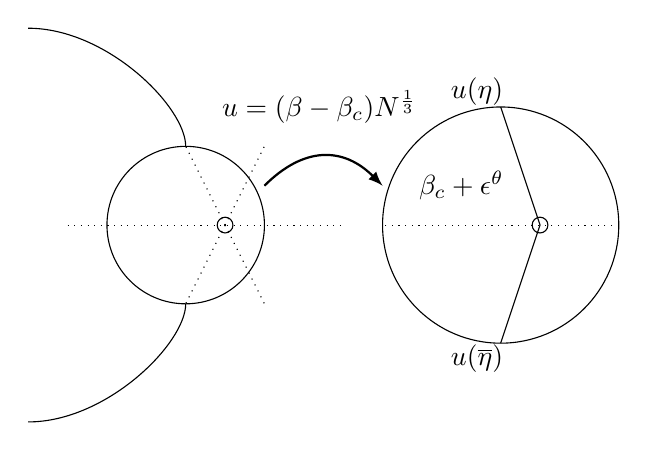
\begin{tikzpicture}
		\draw[draw=black, thin, solid] (-3.50,0.50) ellipse (1.00 and 1.00);
		\draw[draw=black, thin, solid] (0.50,0.50) ellipse (1.50 and 1.50);
		\draw[draw=black, thin, solid] (-5.50,3.00) .. controls (-4.50, 3.00) and (-3.50, 2.00) .. (-3.50,1.50);
		\draw[draw=black, thin, solid] (-5.50,-2.00) .. controls (-4.50, -2.00) and (-3.50, -1.00) .. (-3.50,-0.50);
		\draw[draw=black, thin, solid] (-3.00,0.50) circle (0.1);
		\draw[draw=black, thin, solid] (1.00,0.50) circle (0.1);
		\draw[draw=black, thin, dotted] (-3.00,0.50) -- (-2.50,1.50);
		\draw[draw=black, thin, dotted] (-3.00,0.50) -- (-3.5,-0.50);
		\draw[draw=black, thin, dotted] (-3.00,0.50) -- (-3.50,1.50);
		\draw[draw=black, thin, dotted] (-3.00,0.50) -- (-2.50,-0.50);
		\draw[draw=black, thin, dotted] (-5.00,0.50) -- (-1.50,0.50);
		\draw[draw=black, thick, -latex, solid] (-2.50,1.00) .. controls (-2.00, 1.50) and (-1.50, 1.50) .. (-1.00,1.00);
		\draw[draw=black, thin, solid] (1.00,0.50) -- (0.50,2.00);
		\draw[draw=black, thin, solid] (1.00,0.50) -- (0.50,-1.00);
		\draw[draw=black, thin, dotted] (2.00,0.50) -- (-1.00,0.50);
		
		\node (Change) at (-1.8,2)    {$u = (\beta - \beta_c)N^{\frac{1}{3}}$};
		\node (Point) at (0,1)    {$\beta_c + \epsilon \ee^{\ii \theta}$};
		\node (ext1) at (0.2,2.2)    {$u(\eta)$};
		\node (ext2) at (0.2,-1.2)    {$u(\overline{\eta})$};
	\end{tikzpicture}
	\label{Figure: Change of local variables, Airy}
\end{figure}
Therefore, taking $\beta = \beta_c + u N^{-\frac{1}{3}}$, for $u$ coming from $\infty \ee^{\ii \frac{4\pi}{3}}$ to $\infty \ee^{\ii \frac{2\pi}{3}}$, we write
\begin{align}
	\He_n(2 N^{\frac{1}{2}} + \xi N^{-\frac{1}{6}}) & = 
	C_n^0 \ee^{\frac{3N}{2}} 
	\int_{\Gamma}  
	\ee^{-N 
		\left(
		\frac{1}{3}(\beta - \beta_c)^3 - \xi \beta N^{-\frac{2}{3}} + \Boh((\beta - \beta_c)^4) 
		\right)}
	\dd \beta 
	\\
	& = C_n^0 \ee^{\frac{3N}{2}} 
	\int_{u(\overline{\eta})}^{u(\eta)}
	\ee^{-N \left(\frac{1}{3}(u N^{-\frac{1}{3}})^3 - \xi (\beta_c + u N^{-\frac{1}{3}}) N^{-\frac{2}{3}} + 
		\Boh((u N^{-\frac{1}{3}})^4) \right)} \dd (u N^{-\frac{1}{3}})
	\\
	& = C_n^0 N^{-\frac{1}{3}} \ee^{-2\xi\beta_c N^{\frac{1}{3}}} \ee^{\frac{3N}{2}}
	\int_{N^{\frac{1}{3}} \ee^{\ii \frac{2\pi}{3}}}^{-N^{\frac{1}{3}} \ee^{\ii \frac{4\pi}{3}}}  \ee^{\frac{1}{3} u^3 - \xi u + \Boh(u^4 N^{-\frac{4}{3}})} \dd u
\end{align}
Then we will have asymptotically in $N$, remembering the definition of the Airy function \ref{Def: Airy Function},
\begin{equation}
	\He_n(2N^{\frac{1}{2}} + \xi N^{-\frac{1}{6}}) = \tilde{C}_N \int_{\rangle}  \ee^{\left(\frac{u^3}{3} - \xi u\right)} \dd u (1 + \boh(1)) = \tilde{C}_N \Ai(\xi) (1 + \boh(1)),
\end{equation}
for
\begin{align}
	\tilde{C}_N & = (N-1)! N^{\frac{1}{6} - \frac{N}{2}} \ee^{-2\xi\beta_c N^{\frac{1}{3}} + \frac{3N}{2}} = \sqrt{2\pi} (N-1)^{\frac{1}{2}} N^{1/6 - N/2} \ee^{\left(1/2 + N^{-1} - 2\xi \beta_c N^{-2/3} \right)} (1 + \Boh(N^{-1})) \\
	& = \sqrt{2\pi\ee} N^{-\frac{N}{2} + \frac{2}{3}} (1 + \Boh(N^{-1})) 
\end{align} 
The result follow from the asymptotic for the Airy function given in \ref{Subsection: Airy Asymptotic}. Again, we can change variables to express
\begin{equation}
	\He_{n-1}(2\sqrt{N} + N^{-1/6}\xi) = \sqrt{2\pi} \ee N^{-\frac{N}{2} + \frac{7}{6}}  \Ai(\xi) (1 + \boh(1))
\end{equation}

\subsection{Kernels}

When dealing with the asymptotic of the j.p.d.f we will actually consider the Kernel. This is the object described in \ref{Theorem: Kernel}. However, we will actually work with the simplification given by \ref{Proposition: Kernel Simplification beta 2}. The first step is to consider the following expression
\begin{equation}
	\He_n(\alpha \sqrt{N} + y N^{-1/2}),
\end{equation}
which will allow us to take the limit to get $K_n^{(2)}(x,x)$.

The computations don't change too much. Consider the expression
\begin{align}
	\He_n(\sqrt{N}\alpha + N^{-1/2} y) & =  \frac{(N-1)! N^{\frac{1}{2}\left(1-N\right)}}{2\pi \ii} \int_{\Gamma}  \ee^{-N(- \alpha \beta+ \frac{1}{2} \beta^2 + \ln{(\beta)}) + y \beta} \dd \beta \\
	& = C_n^0 \int_{\Gamma}  \ee^{-N \phi_\alpha(\beta) + y \beta} \dd \beta \\
	& = C_n^0 \int_{\Gamma}  \ee^{-N \phi_\alpha(\beta)} g_y(\beta) \dd \beta
	\label{Equation: Hermite Integral}
\end{align}
with 
\begin{equation}
	\phi_\alpha(\beta) = \frac{1}{2} \beta^2 - \alpha \beta + \ln{(\beta)}; \quad g_y(\beta) = \ee^{y \beta}
\end{equation}
The analysis remains the same - the difference now being that we have a function $g_y(\beta)$ that enters in the steepest descent expression. Setting our case for $-2\sqrt{N} < x < 2\sqrt{N}$, or, equivalently, $-2 < \alpha < 2$, we remember that $\beta_c^\pm = \ee^{\pm \ii \gamma}$. Now, with this, and setting $\Delta = 2\sqrt{N}\cos(\gamma) + N^{-1/2} y$,
\begin{equation}
	\begin{split}
		\He_n(\Delta) &= C_n^0 \int_{\Gamma}  \ee^{-N \phi_\alpha(\beta)} g_y(\beta) \dd \beta  = C_n^0  \left[ \int_{\Gamma_d^-}  \ee^{-N \phi_\alpha(\beta)} g_y(\beta) \dd \beta + \int_{\Gamma_d^+}  \ee^{-N \phi_\alpha(\beta)} g_y(\beta) \dd \beta  \right]\\
		& \stackrel{(Steepest)}{=}  
		C_n^0 \left(
		\ee^{-N(\phi_\alpha(\beta_c^+))} 
		\left[
		\frac{\sqrt{2\pi}}{N^{\frac{1}{2}}}
		\frac{g_y(\beta^+_c) \ee^{\ii (\theta(\beta_c^+))}}{\sqrt{2\sin{(\gamma)}}} 
		+ \Boh(N^{-\frac{3}{2}})
		\right]
		+
		\ee^{-N(\overline{\phi_\alpha(\beta_c^+)})} 
		\left[
		\frac{\sqrt{2\pi}}{N^{\frac{1}{2}}}
		\frac{g_y(\beta^-_c) \ee^{\ii (\overline{\theta(\beta_c^+)})}}{\sqrt{2\sin{(\gamma)}}}
		+ \Boh(N^{-\frac{3}{2}})
		\right]   
		\right)
		\\
		& = C_n^0 \sqrt{\frac{2\pi}{2N\sin{(\gamma)}}} \left(
		\ee^{-N(\phi_\alpha(\beta_c^+))} 
		\left[
		g_y(\beta^+_c)
		\ee^{\ii(\theta(\beta_c^+))} 
		+ \Boh(N^{-1})
		\right]
		+
		\ee^{-N(\overline{\phi_\alpha(\beta_c^+)})} 
		\left[
		g_y(\beta^-_c)
		\ee^{\ii(\overline{\theta(\beta_c^+)})}
		+ \Boh(N^{-1})
		\right]   
		\right)
		\\
		& = C_n^0 \sqrt{\frac{\pi}{N\sin{(\gamma)}}} \ee^{y \cos{(\gamma)}}
		\left(
		\ee^{-N(\phi_\alpha(\beta_c^+)) + \ii(\theta(\beta_c^+) + y \sin{(\gamma)})} +
		\ee^{-N(\overline{\phi_\alpha(\beta_c^+)})+\ii(\overline{\theta(\beta_c^+)} - y \sin{(\gamma)})} 
		\right)
		(1 + \Boh(N^{-1}))   
		\\
		%		& =  C_n^0 \sqrt{\frac{\pi}{N\sin{(\gamma)}}} \ee^{y\cos{(\gamma)}}
		%		\left(
		%		\ee^{-\ii(\theta(\beta_c^+) - y \sin{(\gamma)}) + N (-\alpha \beta_c^+ + \frac{1}{2} (\beta_c^+)^2 + \ln{(\beta_c^+)}) }
		%		+
		%		\ee^{\ii \pi} \ee^{\ii(\theta(\beta_c^+) - y \sin{(\gamma)}) + N \overline{(-\alpha \beta_c^+ + \frac{1}{2} (\beta_c^+)^2 + \ln{(\beta_c^+)}) }}  
		%		\right)
		%		(1 + \Boh(N^{-1})) 
		%		\\
		%		& =  C_n^0 \sqrt{\frac{\pi}{N\sin{(\gamma)}}}
		%		\ee^{y\cos{(\gamma)}} \ee^{N(-\cos^2{(\gamma)} - \frac{1}{2})}
		%		\left(
		%		\ee^{-\ii \left(-N\left(\frac{\sin{(2\gamma)}}{2}-\gamma\right)+ \theta(\beta_c^+) - y \sin{(\gamma)}
			%		\right)}
		%		-
		%		\ee^{\ii
			%			\left(-N\left(\frac{\sin{(2\gamma)}}{2}-\gamma\right)+
			%			\theta(\beta_c^+) - y \sin{(\gamma)}
			%			\right)}  
		%		\right)
		%		(1 + \Boh(N^{-1})) 
		%		\\
		& =  C_n^0 \sqrt{\frac{\pi}{N\sin{(\gamma)}}}
		\ee^{y\cos{(\gamma)}}
		\ee^{N(\cos^2{(\gamma)} + \frac{1}{2})}
		2\ii \sin{\left(\theta(\beta_c^+) + y \sin{(\gamma)}
			-N\left(\frac{\sin{(2\gamma)}}{2}-\gamma\right)\right)} 
		(1 + \Boh(N^{-1})) \\
		& = \frac{(N-1)! N^{\frac{1}{2}\left(1-N\right)}}{2\pi \ii}
		\sqrt{\frac{\pi}{N\sin{(\gamma)}}} 
		\ee^{y\cos{(\gamma)}}
		\ee^{N(\cos^2{(\gamma)} + \frac{1}{2})}
		2\ii \sin{
			\left(
			\theta(\beta_c^+) + y \sin{(\gamma)}
			-N\left(\frac{\sin{(2\gamma)}}{2}-\gamma\right)
			\right)} 
		(1 + \Boh(N^{-1})) \\
		%		& = \sqrt{\frac{2}{\sin{(\gamma)}}} N^{-\frac{N}{2}} (N-1)^{\left(N - \frac{1}{2}\right)}
		%		\ee^{N\left(-\cos^2{(\gamma)} + \frac{1}{2} \right) + 1 + y\cos{(\gamma)}} \sin{\left(\theta(\beta_c^+) + y \sin{(\gamma)}-N\left(\frac{\sin{(2\gamma)}}{2}-\gamma\right)\right)} 
		%		(1 + \Boh(N^{-1})) \\
		& = \sqrt{\frac{2}{\sin{(\gamma)}}} N^{\frac{1}{2}\left(N - 1\right)}
		\ee^{N\left(\cos^2{(\gamma)} - \frac{1}{2} \right)  + y\cos{(\gamma)}} \sin{\left(\theta(\beta_c^+) + y \sin{(\gamma)}-N\left(\frac{\sin{(2\gamma)}}{2}-\gamma\right)\right)} 
		(1 + \Boh(N^{-1}))
	\end{split}
\end{equation}
and for $N-1$,
\begin{equation}
	\He_{n-1}(\Delta) = \sqrt{\frac{2}{\sin{(\gamma)}}} N^{\frac{1}{2}(N - 2)} \frac{\ee^{N\left(\cos^2{(\gamma)} - \frac{1}{2} \right) + y\cos{(\gamma)}}}{\ee^{\cos^2{(\gamma)}}} \sin{\left(\theta(\beta_c^+) + y \sin{(\gamma)} - (N-1) \left(\frac{\sin{(2\gamma)}}{2}-\gamma\right)\right)} 
	(1 + \Boh(N^{-1}))
\end{equation}

Remembering the expression for the Kernel, taking $\Delta_x = \sqrt{N}\alpha + N^{-1/2} x$ and $\Delta_y = \sqrt{N}\alpha + N^{-1/2} y$
\begin{align}
	K_n^{(2)}(\Delta_x,\Delta_y) & = \frac{\sqrt{\wf(\Delta_x) \wf(\Delta_y)}}{r_{n-1}^{(2)}} \frac{H_n(\Delta_x)H_{n-1}(\Delta_y) - H_{n-1}(\Delta_x)H_n(\Delta_y)}{\Delta_x-\Delta_y} \\
	& = W_{(N,x,y)} \frac{H_n(\Delta_x)H_{n-1}(\Delta_y) - H_{n-1}(\Delta_x)H_n(\Delta_y)}{(\sqrt{N}\alpha + N^{-1/2} x)-(\sqrt{N}\alpha + N^{-1/2} y)} \\
	& = W_{(N,x,y)} N^{1/2} \frac{H_n(\Delta_x)H_{n-1}(\Delta_y) - H_{n-1}(\Delta_x)H_n(\Delta_y)}{x-y}
\end{align}
with 
\begin{align}
	W_{(N,x,y)} & = \frac{\sqrt{\wf(\sqrt{N}\alpha + N^{-1/2} x) \wf(\sqrt{N}\alpha + N^{-1/2} y)}}{r_{n-1}^{(2)}} \\
	& = \frac{1}{(N-2)!} \left(\frac{\exp{\left( -\frac{1}{2} \left(\sqrt{N}\alpha + N^{-1/2} x \right)^2 \right)}}{\sqrt{2\pi}}  \frac{\exp{\left( -\frac{1}{2} \left(\sqrt{N}\alpha + N^{-1/2} y \right)^2 \right)}}{\sqrt{2\pi}} \right)^{\frac{1}{2}} \\
	& = \frac{1}{\sqrt{2\pi} (N-2)!} \left( \exp{\left\{ -\frac{1}{2} \left( 4 N \cos^2{(\gamma)} + 4 x \cos{(\gamma)} + x^2 N^{-1} + 4 N \cos^2{(\gamma)} + 4 y \cos{(\gamma)} + y^2 N^{-1} \right) \right\}} \right)^{\frac{1}{2}} \\
	& = \frac{1}{\sqrt{2\pi} (N-2)!} \left( \exp{\left\{ - \left( 2N \cos^2{(\gamma)} + 2 x \cos{(\gamma)} + x^2 (2N)^{-1} + 2 N \cos^2{(\gamma)} + 2 y \cos{(\gamma)} + y^2 (2N)^{-1} \right) \right\}} \right)^{\frac{1}{2}} \\
	& = \frac{\ee^{-2N\cos^2{(\gamma)}}}{\sqrt{2\pi} (N-2)!}
	\exp{\left\{-\cos{(\gamma)} (x+y) - \frac{1}{4N} (x^2 + y^2) \right\}} 
\end{align}
Note that
\begin{equation}
	H_n(\Delta_x)H_{n-1}(\Delta_y) \propto \sin{\left(\theta(\beta_c^+) + x \sin{(\gamma)}-N\left(\frac{\sin{(2\gamma)}}{2}-\gamma\right)\right)} \sin{\left(\theta(\beta_c^+) + y \sin{(\gamma)} - (N-1) \left(\frac{\sin{(2\gamma)}}{2}-\gamma\right)\right)} 
\end{equation}
and
\begin{equation}
	H_{n-1}(\Delta_x)H_n(\Delta_y) \propto \sin{\left(\theta(\beta_c^+) + y \sin{(\gamma)}- N\left(\frac{\sin{(2\gamma)}}{2}+ \gamma\right)\right)} \sin{\left(\theta(\beta_c^+) + x \sin{(\gamma)} - (N-1) \left(\frac{\sin{(2\gamma)}}{2}-\gamma\right)\right)} 
\end{equation}
therefore,
\begin{equation}
	H_n(\Delta_x)H_{n-1}(\Delta_y) - H_{n-1}(\Delta_x)H_n(\Delta_y) \propto \sin{\left(\frac{\sin{(2\gamma)}}{2}-\gamma\right)} \sin{\left( \sin{(\gamma)}(x - y) \right)}
\end{equation}
Then, letting $x' = x \sin{(\gamma)}$ and $y' = y \sin{(\gamma)}$
\begin{align}
	K_n^{(2)}(\Delta_{x'},\Delta_{y'}) & = W_{(N,x',y')} N^{1/2} C \ee^{\cos{(\gamma)}\sin{(\gamma)}(x' + y')} \frac{\sin{\left(\frac{\sin{(2\gamma)}}{2}-\gamma\right)} }{\sin{(\gamma)}}\frac{\sin{(x' - y')}}{x'-y'}
\end{align}
where
\begin{align}
	C & = \left(\sqrt{\frac{2}{\sin{(\gamma)}}}
	N^{\frac{1}{2}(N-1)}
	\ee^{N\left(\cos^2{(\gamma)} - \frac{1}{2} \right)} \right) 
	\left( \sqrt{\frac{2}{\sin{(\gamma)}}} 
	N^{\frac{1}{2}(N-2)}
	\frac{\ee^{N\left(\cos^2{(\gamma)} - \frac{1}{2} \right)}}{\ee^{\cos^2{(\gamma)} }}
	\right) \\
	& = \frac{2}{\sin{(\gamma)}}
	N^{N - \frac{3}{2}}
	\frac{\ee^{2N\left(\cos^2{(\gamma)} - \frac{1}{2} \right)}}{\ee^{\cos^2{(\gamma)}}}
\end{align}
and
\begin{equation}
	W_{(N,x',y')} = \frac{\ee^{-2N\cos^2{(\gamma)}}}{\sqrt{2\pi} (N-2)!}
	\exp{\left\{-\sin{(\gamma)}\cos{(\gamma)} (x'+y') - \frac{\sin^2{(\gamma)}}{4N} (x'^2 + y'^2) \right\}} 
\end{equation}
Here, we get to the point of interest. 
\begin{definicao}
	The Kernel
	\begin{equation}
		\Sine(x, y) \deff \frac{\sin{(x  -y)}}{x - y}
	\end{equation}
	is called the \textit{Sine Kernel}.
\end{definicao}
With this definition, we can now say that 
\begin{teorema}
	For the conditions $-2\sqrt{N} < x < 2\sqrt{N}$, or, equivalently, $-2 < \alpha < 2$, we remember that $\beta_c^\pm = \ee^{\pm \ii \gamma}$. Set $\Delta_x = 2\sqrt{N}\cos(\gamma) + \frac{\sin{(\gamma)}}{\sqrt{N}} x$ and $\Delta_y = 2\sqrt{N}\cos(\gamma) + \frac{\sin{(\gamma)}}{\sqrt{N}} y$. Then, we have that
	\begin{equation}
		K_n^{(2)}\left(\Delta_x, \Delta_y\right) = \frac{\sin{\left(\frac{\sin{(2\gamma)}}{2}-\gamma\right)}}{\ee^{\cos^2{(\gamma)}} \pi \sin^2{(\gamma)}} \Sine(x, y) (1 + \Boh(N^{-1}))
	\end{equation}
\end{teorema}

\subsection{Equilibrium Measure}

Remember in \ref{Subsection: The case for beta 2} when we expressed the equilibrium measure in terms of the Kernel of the point process - given in \ref{Equation: Equilibrium Measure and Kernel}. It was noted then that we would only need to understand the asymptotics of the orthogonal polynomial associated with the weight function to properly recover the equilibrium measure. Now, we have such an asymptotic. Remember the expression
\begin{equation}
	\pe^{(w)}(x) = K_n^{(2)}(x, x) = \frac{\wf(x)}{r_{n-1}^{(2)}} \left( \He_{n-1}(x)\partial_x \He_n(x) - \He_{n}(x)\partial_x \He_{n-1}(x)  \right)
\end{equation}
We will make use of the following relation
\begin{definicao}
	The Hermite polynomial satisfies the following propertie
	\begin{equation}
		\partial_x \He_{n}(x) = n \He_{n-1}(x)
	\end{equation}
\end{definicao}
\begin{proof}
	\begin{align}
		\frac{\dd}{\dd x} \He_n(x) & = \frac{\dd}{\dd x} \left( (-1)^{(n)}\ee^{\frac{1}{2} x^2} \frac{\dd^n}{\dd x^n} \ee^{-\frac{1}{2} x^2} \right) \\
		& = (-1)^{(n)}  \left( x \ee^{\frac{1}{2} x^2} \frac{\dd^n}{\dd x^n} \ee^{-\frac{1}{2} x^2} +  \ee^{\frac{1}{2} x^2} \frac{\dd^{n+1}}{\dd x^{n+1}} \ee^{-\frac{1}{2} x^2}  \right) \\
		& =  x \left( (-1)^{(n)}  \ee^{\frac{1}{2} x^2} \frac{\dd^n}{\dd x^n} \ee^{-\frac{1}{2} x^2} \right) -   (-1)^{(n+1)} \left(  \ee^{\frac{1}{2} x^2} \frac{\dd^{n+1}}{\dd x^{n+1}} \ee^{-\frac{1}{2} x^2} \right)  \\
		& = x \He_n(x) - \He_{n+1}(x) \\
		& = x \He_n(x) - \left(  x\He_n(x) - n \He_{n-1}(x) \right) \\
		& =  n \He_{n-1}(x) 
	\end{align}
\end{proof}
using this result, one can write that
\begin{align}
	\pe^{(w)}(x) = K_n^{(2)}(x, x) & = \frac{\wf(x)}{r_{n-1}^{(2)}} \left( He_{n-1}(x)  n \He_{n-1}(x) - \He_{n}(x)(n-1) \He_{n-2}(x)   \right) \\
	& = \frac{\wf(x)}{r_{n-1}^{(2)}} \left( n \He^2_{n-1}(x) - (n-1)  \He_{n}(x)\He_{n-2}(x)   \right) \\
	& = \frac{\wf(x)}{r_{n-1}^{(2)}} \left( (N-1) \He^2_{n-1}(x) - (N-2)  \He_{n}(x)\He_{n-2}(x)   \right) \\
\end{align}
and now it suffices to have the expression for $\He_{n-2}(x)$.
\begin{equation}
	\He_n(2\sqrt{N}\cos{(\gamma)}) = \sqrt{\frac{2}{\sin{(\gamma)}}}
	N^{\frac{1}{2} \left(N - 1\right)}
	\ee^{N\left(\cos^2{(\gamma)} - \frac{1}{2} \right)} 
	\sin{
		\left(
		\theta(\beta_c^+) 
		-N\left(\frac{\sin{(2\gamma)}}{2}
		-\gamma\right)
		\right)
	} 
	(1 + \Boh(N^{-1}))
\end{equation}
\begin{equation}
	\He_{n-1}(2\sqrt{N}\cos(\gamma)) = \sqrt{\frac{2}{\sin{(\gamma)}}}
	N^{\frac{1}{2} \left(N -2\right)}
	\frac{\ee^{N\left(\cos^2{(\gamma)} - \frac{1}{2} \right)}}{\ee^{\cos^2{(\gamma)}}}
	\sin{
		\left(
		\theta(\beta_c^+) 
		-(N-1)\left(\frac{\sin{(2\gamma)}}{2}
		-\gamma\right)
		\right)
	} 
	(1 + \Boh(N^{-1}))
\end{equation}
\begin{equation}
	\He_{n-2}(2\sqrt{N}\cos(\gamma)) = \sqrt{\frac{2}{\sin{(\gamma)}}}
	N^{\frac{1}{2} \left(N - 3\right)}
	\frac{\ee^{N\left(\cos^2{(\gamma)} - \frac{1}{2} \right)}}{\ee^{2\cos^2{(\gamma)}}}
	\sin{
		\left(
		\theta(\beta_c^+) 
		-(N-2)\left(\frac{\sin{(2\gamma)}}{2}
		-\gamma\right)
		\right)
	} 
	(1 + \Boh(N^{-1}))
\end{equation}
Therefore
\begin{align}
	\pe^{(w)}(x) & =  \Pi_N \left[(N-1) \sin^2{\left(\theta(\beta_c^+)-(N-1)\Theta \right)} - (N-2) \sin{\left(\theta(\beta_c^+)-(N-2)\Theta\right)}  \sin{\left(\theta(\beta_c^+)-N\Theta \right)} \right] \\
	& =  \Pi_N N \left[\sin^2{\left(\theta(\beta_c^+)-(N-1)\Theta \right)} - \sin{\left(\theta(\beta_c^+)-(N-2)\Theta\right)}  \sin{\left(\theta(\beta_c^+)-N\Theta \right)} \right] \left(1 + \Boh(1) \right)
\end{align}
with
\begin{align}
	\Pi_N & = \frac{\ee^{-\frac{1}{2}\left(2\cos{\gamma}\sqrt{N}\right)^2}}{(N-2)!} \left( \frac{2}{\sin(\gamma)} 	\frac{\ee^{2N\left(\cos^2{(\gamma)} - \frac{1}{2} \right)}}{\ee^{2\cos^2{(\gamma)}}} N^{N-2}\right) \\
	& = \frac{2 \ee^{-2\cos^2{(\gamma)}}}{\sin(\gamma) \sqrt{2\pi N}} \\
\end{align} 
and
\begin{equation}
	\Theta = \left(\frac{\sin{(2\gamma)}}{2}+\gamma\right)
\end{equation}
Finally, using the identity $\cos^2(a + b) - \cos(a)\cos(a+2b) = \sin^2(b)$,
\begin{align}
	\pe^{(w)}(\alpha) & =  \frac{2 \ee^{-2\cos^2{(\gamma)}}}{\sin(\gamma) \sqrt{2\pi N}} \left[\sin^2{\left(\theta(\beta_c^+)-(N-1)\Theta \right)} - \sin{\left(\theta(\beta_c^+)-(N-2)\Theta\right)}  \sin{\left(\theta(\beta_c^+)-N\Theta \right)} \right] \left(1 + \Boh(1) \right) \\
	& =  \frac{2 \ee^{-2\cos^2{(\gamma)}}}{\sin(\gamma) \sqrt{2\pi N}} \left[\cos^2{\left(a + \gamma \right)} - \cos{\left( a \right)} \cos{\left(a + 2\gamma \right)}  \right] \left(1 + \Boh(1) \right) \\
	& =  \frac{2 \ee^{-2\cos^2{(\gamma)}}}{\sin(\gamma) \sqrt{2\pi N}} \sin^2{(\gamma)} \left(1 + \Boh(1) \right) \\
	& = \frac{2 \ee^{-2\cos^2{(\gamma)}}}{ \sqrt{2\pi N}} \sin{(\gamma)} \left(1 + \Boh(1) \right) \\
	& = \frac{\ee^{-\frac{1}{2}\alpha^2}}{\sqrt{2\pi N}} \sqrt{4 - \alpha^2}
\end{align}
using that
\begin{equation}
	a - \frac{\pi}{2} = \theta(\beta_c^+) - N \Theta - \frac{\sin{(2\gamma)}}{2}
\end{equation}
}

\section{Asymptotic on Integrals}

The techniques we will expand on here refers to a specific type of complex function $\phi(\lambda): \C \rightarrow \R$ in the regimen where $\lambda \rightarrow \infty$. Those functions are of the form 
\begin{equation}
	\phi(\lambda) := \int_{\Gamma} g(s) \ee^{-\lambda f(s)} \dd s,
	\label{Equation: Integral form phi}
\end{equation}
where $\Gamma$ is a given contour in the plane and $f, g$ are suitable functions. Suitable here means that we impose $g$ and $f$ to be continuous (or analytic); $g$ is integrable; $f$ have global minima with zero derivative (maybe in more than one point) and strictly positive second derivative at this point(s) of maximum. There is also a more technical regularity condition on $f$ to ensure the approximations holds to still be made clear.

These conditions are not unnatural. Firstly, one can determine a large class of functions to which all of the requirements hold. Consider for example the following example.

\begin{exemplo}
	(Airy Equation) Consider the function which satisfies the equation $\psi''(x) = x \psi(x)$. Taking the Fourrier transform we have 
	\begin{equation}
		-\omega^2 \Phi(x) = \ii \Phi'(x)
	\end{equation}
	for which we can solve for $\Phi(x) $ and then take the inverse Fourrier Transform to get 
	\begin{equation}
		\phi(x) = \frac{1}{2\pi} \int_{-\infty}^{\infty} \ee^{\ii/3 \omega^3 + \ii x \omega} \dd \omega.
	\end{equation}
 	The imaginary part of the argument is an odd function and therefore zero when integrated. The rest is expressed 
	\begin{equation}
		\phi(x) = \frac{1}{2\pi} \int_{-\infty}^{\infty} \cos{\left( \frac{\omega^3}{3} + x \omega \right)} \dd \omega.
	\end{equation}
 But how to know if this is the only solution? One can prove that for a more general definition of a Transform 
\begin{equation}
	\tilde{F} f(w) := \frac{1}{\sqrt{2\pi \ii}} \int_{\Gamma} \ee^{-\ii \omega s} f(s) \dd s
\end{equation}
 holds very similar properties of the Fourier Transformation and solves the equation for any contour that gives a convergent integral. We can actually choose independent contour such that each give us a different independent solution to the equation. More importantly, for this integral, the techniques applied here are of great use to understand its behavior as $\omega \rightarrow \infty$.
\end{exemplo}

Moreover, one can somehow directly motive such conditions. Consider $\phi(\lambda): \R \rightarrow \R$, $f$ with a single global minima and $\Gamma \equiv \R$ - for simplicity; the argument's idea should hold given the appropriate considerations. If $\phi$ is as in \autoref{Equation: Integral form phi}, and satisfying the conditions given for such function. Then, take $x^*$ the single maximum critical point for $f$. We first note that if that is true, then, for any $|\epsilon| > 0$, the following limit should hold:
\begin{equation}
	\lim_{\lambda \rightarrow \infty} \frac{\ee^{-\lambda(f(x^*))}}{\ee^{-\lambda(f(x^* - \epsilon))}} = \lim_{\lambda \rightarrow \infty} \ee^{-\lambda(f(x^*) - f(x^* - \epsilon))} = \lim_{\lambda \rightarrow \infty} \ee^{\lambda |c|} \rightarrow + \infty. 
\end{equation}
That is, the main contribution for the integral comes from a single point. The main idea then is to separate the integral in two regions: A first interval $(x^* - c/\sqrt{\lambda}, x^* + c/\sqrt{\lambda}), c > 0$, including this critical point and another interval that in theory should contribute only in error for the integral asymptotic. We start by approximating $f$ around its global maximum by Taylor's theorem 
	\begin{equation}
		f(x) = f(x^*) - \frac{1}{2} |f''(x^*)|(x-x^*)^2 + \epsilon_2(x-x^*)
	\end{equation}
	and then perform a change of variables $\frac{x}{\sqrt{\lambda}} = s - x^*$, so that 
	\begin{equation}
		\int_{x^*-\frac{c}{\sqrt{\lambda}}}^{x^*+\frac{c}{\sqrt{\lambda}}} g(s) \ee^{-\lambda f(s)} \dd(s) = \frac{\ee^{-\lambda f(x^*)}}{\sqrt{\lambda}} \int_{-c}^c g\left(x^* + \frac{x}{\sqrt{\lambda}}\right) \ee^{\frac{1}{2} |f''(x^*)|x^2 - \epsilon_2\left(\frac{x^3}{\sqrt{\lambda}}\right)} \dd x.
	\end{equation}
	Now, using the technical assumption of regularity on the function $f$, one can argue that the error term $\epsilon_2$ goes to zero sufficiently fast, leaving a Gaussian Integral. More that that, one need to argue that the integral outside this small neighborhood of $x^*$ is exponentially smaller then $\ee^{\lambda \phi(x^*)}$. This should follow by an argument where the asymptotic for the integral 
	\begin{equation}
			\int_{x^*+ \frac{c}{\sqrt{\lambda}}}^{\infty} g(s) \ee^{-\lambda f(s)} \dd(s) \leq \ee^{-\lambda f(x^*+ \frac{c}{\sqrt{\lambda}})} \normL{1}{g}
	\end{equation}
	is exponentially less than the previous region. 
	
	With this, we only note a few details of interest. Firstly, more precise error estimates can be obtained if one uses higher order terms of the Taylor Series expansion of $f$. For maximizer $x^*$ which have null second derivative (a double critical point), the Laplace Approximation can be used expanding to the third order terms of the Taylor Series $f(x) = f(x^*) = \frac{1}{6}f'''(x^*)(x-x^*)^3 + \epsilon_3(x-x^*)$ and making the change of variables $t/\sqrt[3]{n} = x - x^*$ instead. This argument and result could also be used on curves on the plane. This is motivated from the fact that every (smooth) curve is locally a straight line. This will lead us to the Method of \textit{Steepest Descent}. These next subsections are in the spirit of proving a bit more formally the expansion given by the Laplace Method and introducing the mentioned Steepest Descent.

\subsection{Watson's Lemma} 

We start this study in the real line by looking at the functions $F: \R \rightarrow \R$ of the form
\begin{equation}
	F(\lambda) = \int_{0}^{T} f(t) \ee^{-\lambda t} \dd t
	\label{equation: F}
\end{equation}
which can be identified as the Laplace transform of a function $f$ supported on $[0,T]$. Note that this function fits well with the models we described previously, that is, it of the form such that one should expect the main contribution to come from the origin given some conditions on $f$. Let's formalize this result.

\begin{teorema}	
	(Watson's Lemma) Take $f \in L^1(0,T)$ and suppose that for some $\delta > 0$ it is of the form
	\begin{equation}
		f(t) = t^\alpha f_0(t), \quad 0 < t \leq \delta,
	\end{equation}
	where $\alpha \in (-1, \infty)$ and $f_0$ is continuously differentiable on $[0, \delta]$ with $f_0(0) \neq 0$. Then the function $F$ in \ref{equation: F} satisfies
	\begin{equation}
		F(\lambda) = \frac{f_0(0) \Gamma(\alpha + 1)}{\lambda^{\alpha + 1}} (1 + \Boh(\lambda^{-1}))
	\end{equation}
	when $\lambda \rightarrow \infty$ and where $\Gamma$ is the Gamma function.
\end{teorema}

\begin{proof}
	A weak estimation of the integral could be given by
	\begin{equation}
		\int_{0}^{T} f(t) \ee^{-\lambda t} \dd t \leq \normL{1}{f}
	\end{equation}
	where we only use the fact that $f \in L^1(0,T)$. However, we have more information on the behavior of the function in the section $0 < t < \delta$. To use this information we start by decomposing the function in two parts
	\begin{equation}
		F(\lambda) = \int_{0}^{\delta} f(t) \ee^{-\lambda t} \dd t + \int_{\delta}^{T} f(t) \ee^{-\lambda t} \dd t \revdeff (1) + (2).
	\end{equation}
	For $(2)$, we can use the same weak estimate, leaving us with 
	\begin{equation}
		F(\lambda) \leq \int_{0}^{\delta} f(t) \ee^{-\lambda t} \dd t + \normL{1}{f} \ee^{-\delta \lambda}.		
	\end{equation}
	Now, we remind of the condition of continuous differentiability and the hypothesis on $f(t)$ to write $(1)$ as
	\begin{align}
		(1) = \int_{0}^{\delta} t^\alpha(f_0(0) + r(t)) \ee^{-\lambda t} \dd t & = f_0(0) \int_{0}^{\delta} t^\alpha \ee^{-\lambda t} \dd t + \int_{0}^{\delta} t^\alpha r(t) \ee^{-\lambda t} \dd t \\
		& \revdeff f_0(0) \cdot (1.1) + (1.2).
	\end{align}
	For these two integrals we can try to simplify the problem by rewriting 
	\begin{align}
	(1.1) & = \int_{0}^{\infty} t^\alpha \ee^{-\lambda t} \dd t - \int_{\delta}^{\infty} t^\alpha \ee^{-\lambda t} \dd t  = \frac{\Gamma(\alpha + 1)}{\lambda^{\alpha +1}} - \int_{\delta}^{\infty} t^\alpha \ee^{-\lambda t} \dd t, \\
	|(1.2)| & \leq \normL{\infty}{f'} \int_{0}^{\delta} t^{\alpha + 1} \ee^{-\lambda t} \dd t \\ &=  \normL{\infty}{f'} \left( \int_{0}^{\infty} t^{\alpha+1} \ee^{-\lambda t} \dd t - \int_{\delta}^{\infty} t^{\alpha+1} \ee^{-\lambda t} \dd t \right) \\
	& =  \normL{\infty}{f'} \left( \frac{\Gamma(\alpha + 2)}{\lambda^{\alpha +2}} - \int_{\delta}^{\infty} t^{\alpha+1} \ee^{-\lambda t} \dd t \right).	
	\end{align}
	where  $\normL{\infty}{f} = \inf{\{ c \geq 0 | \mu(\{|f| > c\}) = 0 \}}$ as usual. We are now only missing one ingredient to get the result, the order of
	\begin{equation}
		G(\lambda, \beta) \deff \int_{\delta}^{\infty} t^{\beta} \ee^{-\lambda t} \dd t, \ \ \ \lambda > 1, \quad \beta > -1. 
	\end{equation}
	Using Cauchy-Schwartz we can estimate
		\begin{align}
			|G(\lambda, \beta)|^2 & \leq \left( \int_{\delta}^{\infty} \ee^{-\lambda t} \dd t \right) \left(\int_{\delta}^{\infty} t^{2\beta} \ee^{-\lambda t} \dd t \right) \\
			& = \left(\frac{e^{-\lambda \delta}}{\lambda}\right) \left( \int_{\delta}^{\infty} t^{2\beta} \ee^{-\lambda t}\dd t \right)	\\
			& \stackrel{(u=\lambda t)}{=} \left(\frac{e^{-\lambda \delta}}{\lambda}\right) \left( \int_{\delta}^{\infty} \ee^{-u} u^{2\beta} \frac{1}{\lambda^{2\beta + 1}} \dd u \right) \\
			& = \frac{\ee^{-\lambda \delta}}{\lambda^{2\beta + 2}} M_\beta
		\end{align}
	where $M_\beta$ is some constant independent of $\lambda$. That leave us with
	\begin{equation}
		G(\lambda, \beta) = \Boh\left(\frac{\ee^{-\lambda\delta/2}}{\lambda^{\beta+1}}\right) = \Boh\left(\ee^{-\epsilon\lambda}\right)
	\end{equation}
	where $\epsilon > 0$ depends on $\beta$ and $\delta$. Finally we can rewrite
	\begin{equation}
		(1.1) = \frac{\Gamma(\alpha + 1)}{\lambda^{\alpha +1}} - G(\lambda, \alpha) =  \frac{\Gamma(\alpha + 1)}{\lambda^{\alpha+1}} + \Boh\left(\ee^{-\epsilon\lambda}\right)
	\end{equation}
	\begin{equation}
		|(1.2)| \leq \normL{\infty}{f'} \left( \frac{\Gamma(\alpha + 2)}{\lambda^{\alpha +2}} - G(\lambda, \alpha + 1) \right) =  \normL{\infty}{f'} \left( \frac{\Gamma(\alpha + 2)}{\lambda^{\alpha +2}} + \Boh\left(\ee^{-\epsilon\lambda}\right) \right) = \Boh\left(\lambda^{-\alpha-2}\right)
	\end{equation}
	and then
	\begin{equation}
		F(\lambda) \leq \Boh\left(\lambda^{-\alpha-2}\right) + f_0(0) \left( \frac{\Gamma(\alpha + 1)}{\lambda^{\alpha+1}} + \Boh\left(\ee^{-\epsilon\lambda}\right) \right) + \normL{1}{f} \ee^{-\delta \lambda}.
	\end{equation}
	By the dominance of the exponential error, we get the result
	\begin{equation}
		F(\lambda) = \frac{f_0(0) \Gamma(\alpha + 1)}{\lambda^{\alpha + 1}} (1 + \Boh(\lambda^{-1}))
	\end{equation}
\end{proof}

In the estimation above, the Gamma function and the factor of $\lambda^{-1}$ is the result of integrating the linear exponent of $\ee{-\lambda t}$. If we, however, change this exponent to be of the general type $-\lambda t^d$ we can still have a similar result on the behavior of the function.

\begin{proposicao}	
	For $T, S > 0$, define the function
	\begin{equation}
		G(\lambda) \deff \int_{-S}^{T} g(t) \ee^{-\lambda t^2} \dd t
	\end{equation}
	and assume $g(x)$ absolutely integrable in $[-S, T]$, of class $C^1$ in a fixed neighborhood of the origin. Then the function satisfies
	\begin{equation}
		G(\lambda) = \frac{g(0) \Gamma(1/2)}{\lambda^{1/2}} + \Boh \left(\frac{1}{\lambda^{3/2}} \right)
	\end{equation}
	when $\lambda \rightarrow \infty$ and where $\Gamma$ is the Gamma function.
	\label{prop: cor watson}
\end{proposicao}

\begin{proof}
	The proof is a reduction of the problem to Watson's Lemma. Assume, $T>S$ and write
	\begin{equation}
		G(\lambda) = \int_{-S}^{S} g(t) \ee^{-\lambda t^2} \dd t + \int_{S}^{T} g(t) \ee^{-\lambda t^2} \dd t
	\end{equation}
	The second integral we know to be of order
	\begin{equation}
		\int_{S}^{T} g(t) \ee^{-\lambda t^2} \dd t \leq ||g||_{\infty} \ee^{-\lambda S^2},
	\end{equation}
	exponential on $\lambda$, so we drop it. For the first integral we rewrite
		\begin{align}
			\int_{-S}^{S} g(t) \ee^{-\lambda t^2} \dd t & = \int_{0}^{S} (g(t) + g(-t)) \ee^{-\lambda t^2}\dd t \\
			& \stackrel{(u= t^2)}{=} \frac{1}{2} \int_{0}^{S^2} \left(\frac{g\left(\sqrt{u}\right) + g\left(-\sqrt{u}\right)}{\sqrt{u}}\right) \ee^{-\lambda u} \dd u
		\end{align}
	where now we can use Watson's Lemma.
\end{proof}

\begin{exemplo}
	Take the function called Gamma given by the expression
	\begin{equation}
		\Gamma(x) = \int_{0}^{\infty} \ee^{-t} t^{x-1} \dd t
		\label{eq: Gamma}
	\end{equation}
	We are interested in what happens to the function when we take the variable $x$ to $+\infty$. To see what happens, let's fit it into Proposition \ref{prop: (Laplace's Method, interior contributions)}. Rewrite equation \ref{eq: Gamma} as
	\begin{equation}
		\int_{0}^{\infty} \ee^{-t+x\log{(t)}-\log{(t)}} \dd t.
	\end{equation} 
	This lead us to identify $\phi$ as $-\log{(t)}$, which would give us $\phi'(t) < 0$, that is, we would have it's minimum at $t=+\infty$. However $\ee^{\log{(t)}} = t^1$ is not integrable near the origin. Something need to change about the identification. Let's introduce a variable to rescale the integral: $xs = t$, s.t.,
	\begin{equation}
		\Gamma(x) = x^x \int_{0}^{\infty} \ee^{-\lambda(s - \log{(s)})} \ee^{-s} \dd s.
	\end{equation}
	Where we have used $\lambda = x - 1$. Thus we identify $\phi(s) = s - \log(s)$ and $g(s) = \ee^{-s}$. in fact, now $\phi$ has a global minima at $s = 1$ and $\phi''(1) = 1 \neq 0$. Hence
	\begin{align}
		\Gamma(x) & = \frac{\sqrt{2\pi} x^x \ee^{-x}}{(x-1)^{(-1/2)}} (1 + \Boh(x^{-1})) \\
		& = \sqrt{2\pi} x^{x - 1/2} \ee^{-x} (1 + \Boh(x^{-1})) \\
		& = (x-1/2)\log{(x)} - x + \frac{1}{2} \log{(2\pi)}
	\end{align}
	Which is called the Stirling formula.
\end{exemplo}

\subsection{Laplace Method}

A seemly natural extension of the type of function we were dealing with are functions of the type
\begin{equation}
	\Phi(\lambda) \deff \int_{a}^{b} g(t) \ee^{-\lambda \phi(t)} \dd t
	\label{equation: Laplace}
\end{equation}
for $a,b \in \R \cup \{-\infty, \infty\}$ and $a<b$. For now, $\phi$ is a real-valued function. To begin the study let's make some assumptions. The first one is that $a$ is finite, that means that we can set $a=0$ without loss of generality. The second assumption is that $\phi$ is a increasing function on $[0,b]$, so that $\phi(0) < \phi(t)$ for any $t$ in the interval. With that we note that the coefficient $\ee^{-\lambda \phi(t)} / \ee^{-\lambda \phi(0)}$ decreases exponentially, that is, the integral is accumulated as the neighborhood of $0$,
\begin{equation}
	\Phi(\lambda) \approx \int_{0}^{\delta} g(t) \ee^{-\lambda \phi(t)} \dd t.
\end{equation}
As we know $\phi(t)$ to be increasing, it's first non zero derivative must be of even order, so that when we expanded the function by Taylor, 
\begin{equation}
\phi(t) \approx \phi(0) + \phi_{2k+1} t^{2k+1}	
\end{equation}
for some $k\geq 0$ and $|t| < \delta$. As $\phi_{2k+1}$, the $(2k+1)$th-derivative, must be positive we also have that, as $\lambda \rightarrow \infty$,
	\begin{align}
		\Phi(\lambda) & \approx \ee^{-\lambda \phi(0)} \int_{0}^{\delta} g(t) \ee^{-\lambda \phi_{2k+1}(t) \cdot t^{2k+1}} \dd t\\
		& \stackrel{(u=t(\lambda \phi_{2k+1})^{1/(2k+1)})}{\approx} \ee^{-\lambda \phi(0)} \frac{g(0)}{(\lambda \phi_{2k+1})^{\frac{1}{2k+1}}} \int_{0}^{\infty} \ee^{-u^{2k+1}} \dd u \\
		& \stackrel{(s=u^{2k+1})}{\approx} \ee^{-\lambda \phi(0)} \frac{g(0)}{ (2k+1)(\lambda \phi_{2k+1})^{\frac{1}{2k+1}}} \int_{0}^{\infty} \ee^{-s} \dd u
	\end{align}
Where the integral can be evaluated as an Gamma function. More than anything we need to focus on an important assumption that was made: that $\phi$ has a global minima at one of the endpoints of integration. Is that were not the case, for example if $a < 0 < b$ and $\phi(t)$ had a global minima at $t=0$ we would now have to consider the expansion
\begin{equation}
\phi(t) \approx \phi(0) + \phi_{2k} t^{2k}	
\end{equation}
which would lead us to the expression
\begin{equation}
\Phi(\lambda) \approx \ee^{-\lambda \phi(0)} \frac{g(0)}{(\lambda \phi_{2k})^{\frac{1}{2k}}} \int_{-\infty}^{\infty} \ee^{-u^{2k}} \dd u	
\end{equation}
which differentiates of the previously result more importantly by the limits of integration. This is closely related to physical boundaries of the problem. Before enunciating the proper Laplace Method we state the Implicit Function Theorem, which will become important in a series of results that follows.

\begin{teorema}
	(Implicit Function Theorem) Assume that $S$ is an open subset of $\R^{n+k}$ and that $F: S \rightarrow \R^k$ is a function of class $C^1$. Assume also that $(a, b)$ is a point in $S$ such that
	\begin{equation}
		F(a, b) = 0, \quad \text{and} \quad \det(D_yF(a,b)\neq 0).
	\end{equation}
	Then
	\begin{enumerate}
		\item There exist $r_0, r_1 > 0$ such hat for every $x \in \R^n$ such that $|x-a| < r_0$, there exists a unique $y \in \R^k$ such that $|y - b| < r_1$
		\begin{equation}
			F(x,y) = 0.
		\end{equation}
		That is, defines a function $y = f(x)$ for $x \in \R^n$ near $a$ with $y = f(x)$ close to $b$.
		\item Moreover, the function $f: B(r_0, a) \rightarrow B(r_1, b) \subset \R^k$ from part $(1)$ is of class $C^1$, and its derivatives may be determined by differentiating the identity 
		\begin{equation}
			F(x, f(x)) = 0
		\end{equation}
		and solving to find the partial derivatives of $f$
	\end{enumerate}
\end{teorema}

Now we turn to our interest.

\begin{teorema}
	(Laplace's Method, endpoint contributions) Let $\Phi$ be as in \ref{equation: Laplace}, with a finite and $g \in L^1(a,b)$. Assume that $\phi$ has a unique global minimum at $t=a$. In addition, suppose that for some $\delta > 0$ and some $\alpha > -1$, the function $g$ takes the form
	\begin{equation}
		g(t) = (t-a)^{\alpha} g_0(t)
	\end{equation}
	for $|t-a| < \delta$ and $g_0$ continuously differentiable in $[a, a+\delta]$ and $g_0(a) \neq 0$, whereas $\phi$ is twice continuously differentiable on $[a, a+\delta]$ with $\phi'(a) > 0$. Then the function $\Phi$ satisfies an estimate of the form
	\begin{equation}
		\Phi(\lambda) = \frac{1}{\lambda^{\alpha + 1}} \frac{g_0(a) \Gamma(\alpha + 1)}{\phi'(a)^{\alpha + 1}} \ee^{-\lambda \phi(a)} \left(1+\Boh(\lambda^{-1})\right)
	\end{equation}
	as $\lambda \rightarrow \infty$.
\end{teorema}

\begin{proof}
	Start by assuming, without loss of generality, that $a=0$ and dividing the integral in two intervals, one in the region where we have information about the behavior of $g$ and another in the rest of the interval,
	\begin{equation}
		\Phi(\lambda) = \int_{0}^{b} g(t) \ee^{-\lambda \phi(t)} \dd t = \int_{0}^{\delta} g(t) \ee^{-\lambda \phi(t)} \dd t + \int_{\delta}^{b} g(t) \ee^{-\lambda \phi(t)} \dd t = (1) + (2).
	\end{equation}
	Knowing that $\phi$ has a global minima at $t = 0$ we can assume, changing $\delta$ as needed, that $\phi(t) > \phi(\delta)$ for any $t > \delta$. That give us a simple limitation for $(2)$:
	\begin{equation}
		(2) = \int_{\delta}^{b} g(t) \ee^{-\lambda \phi(t)} \dd t \leq \ee^{-\lambda \phi(\delta)} \int_{\delta}^{b} g(t) \dd t \leq \ee^{-\lambda \phi(\delta)} \normL{1[0,b]}{g}.
	\end{equation}
	We now get back to $(1)$ and start by studying the difference give by $\phi(t) - \phi(0) = s$ in a similar way that we would think of a change of variable. Define the multivariate function
	\begin{equation}
		H(t,s) \deff \phi(t) - \phi(0) - s
	\end{equation} 
	such that $H(0,0) = 0$ and $\partial_t H(0,0) \neq 0$. This means we are in the condition to use the Theorem of the Implicit Function to say that there exists a unique bijective and continuously differentiable function $t(s) \deff t$ such that 
	\begin{equation}
		\begin{cases}
			\phi(t(s)) - \phi(0) - s = 0,	\\
			t'(0) = \frac{\partial_s H(0,0)}{\partial_t H(0,0)} = \frac{1}{\phi'(0)}.
		\end{cases}
	\end{equation}
	If we set $T = t^{-1}(\delta)$ we would then have
	\begin{equation}
		\int_{0}^{\delta} g(s) \ee^{-\lambda \phi(s)} \dd s = \int_{0}^{T} g(t(s)) \ee^{-\lambda \phi(t(s))} t'(s) \dd s,
	\end{equation}
	for now to apply the assumption on $g$. We write $g(t(s)) = t^\alpha(s) g_0(t(s))$ and because of its Taylor expansion,
	\begin{equation}
	t(s) = s t'(0) (1+r(s)) = \frac{s}{\phi'(0)}(1+r(s)).		
	\end{equation}
	Joining both results,
		\begin{align}
			\int_{0}^{T} g(t(s)) \ee^{-\lambda \phi(t(s))} t'(s) \dd s & = \ee^{\lambda \phi(0)} \int_{0}^{T} g(t(s)) \ee^{-\lambda (\phi(t(s)) - \phi(0))} t'(s) \dd s \\
			& = \ee^{\lambda \phi(0)} \int_{0}^{T} t^\alpha(s) g_0(t(s)) \ee^{-\lambda s} t'(s) \dd s \\
			& = \frac{\ee^{\lambda \phi(0)}}{\phi'(0)^\alpha} \int_{0}^{T} s^\alpha (1+r(s))^\alpha g_0(t(s)) \ee^{-\lambda s} t'(s) \dd s			
		\end{align}
	where, if we set $f(s) \deff s^\alpha (1+r(s))^\alpha g_0(t(s))$ we can apply Watson's Lemma.
\end{proof}

\begin{teorema}
	(Laplace's Method, interior contributions) Let $\Phi$ be as in \ref{equation: Laplace}, with a finite and $g \in L^1(a,b)$. Assume that $\phi$ has a unique global minimum at $t=c \in (a,b)$. In addition, suppose that for some $\delta > 0$ and some $\alpha > -1$, the function $g$ takes the form
	\begin{equation}
		g(t) = (t-a)^{\alpha} g_0(t)
	\end{equation}
	for $|t-a| < \delta$ and $g_0$ continuously differentiable in $[c-\delta, c+\delta]$ and $g_0(a) \neq 0$, whereas $\phi$ is three times continuously differentiable on $[c-\delta, c+\delta]$ with $\phi'(a) > 0$. Then the function $\Phi$ satisfies an estimate of the form
	\begin{equation}
		\Phi(\lambda) = \ee^{-\lambda \phi(c)} \left( \frac{\sqrt{2\pi} g(c)}{\sqrt{|\phi''(c)|}\lambda^{1/2}} + \Boh(\lambda^{-3/2})\right)
	\end{equation}
	as $\lambda \rightarrow \infty$.
	\label{prop: (Laplace's Method, interior contributions)}
\end{teorema}

\begin{proof}
	Although the proof may be similar there is an important distinction in the solution. Suppose we wanted to try the same approach. We would first assume, w.l.g., that c = 0. Then, we could write
	\begin{align}
	\Phi(\lambda) & = \int_{a}^{b} g(t) \ee^{-\lambda \phi(t)} \dd t \\ 
	& = \int_{a}^{-\delta} g(t) \ee^{-\lambda \phi(t)} \dd t + \int_{-\delta}^{\delta} g(t) \ee^{-\lambda \phi(t)} \dd t + \int_{\delta}^{b} g(t) \ee^{-\lambda \phi(t)} \dd t\\
	&  \revdeff (1) + (2) + (3).		
	\end{align}
	For $(1)$ and $(3)$ the result is as it was before
	\begin{equation}
		\begin{cases}
			(1)	= \int_{\delta}^{a} g(-t) \ee^{-\lambda \phi(-t)} \dd t \leq \ee^{\lambda \phi(-\delta)} ||g||_{L^1[a,b]}\\
			(3) = \int_{\delta}^{b} g(t) \ee^{-\lambda \phi(t)} \dd t \leq \ee^{\lambda \phi(\delta)} ||g||_{L^1[a,b]}
		\end{cases}
	\end{equation}
	For $(2)$ we would try to define a function
	\begin{equation}
		H(t,s) \deff \phi(t) - \phi(0) - s^2.		
	\end{equation} 
	However we could not apply the Implicit Function Theorem here as its derivative $\partial_t H = \phi'$ vanishes at $t=0$. A nice fact about this indetermination is that it doesn't come from the fact that there are no solutions to $H(t,s) = 0$ but from the fact that there are two. To solve this we will use a technique called \textit{blow up}. First, we introduce a variable $v = v(t)$ such that $vs = t$. Now, we redefine our function of interested to be
	\begin{equation}
		L(s, v) \deff \frac{\phi(sv) - \phi(0)}{s^2} - 1.		
	\end{equation}
	for $s\in(-\delta, \delta) - \{0\}$. We would think this function is also singular but note that, using the Taylor Expansion of $\phi$ we can write
	\begin{equation}
		\phi(t) = \frac{\phi''(0)}{2}t^2 + t^3R(t)
	\end{equation}	
	which leave us with 
	\begin{equation}
		L(s, v) = \frac{\phi''(0)}{2}v^2 + sv^3R(sv) - 1
	\end{equation}
	where we can indeed apply the Implicit Function Theorem. In fact, we know $L \in C^2$ and as we want to solve for $L(s,v) = 0$, we need that the $v_0$ we take to satisfy $L(0, v_0) = 0$, ie,
	\begin{equation}
		v_0 = \sqrt{\frac{2}{\phi''(0)}}.
	\end{equation}
	Now, we also know that
	\begin{equation}
		\partial_v L(0, v_0) = \phi''(0) v_0 \neq 0.
	\end{equation}
	So we get a bijective and continuously differentiable function $v = v(s)$ such that
	\begin{equation}
		\begin{cases}
			L(s, v(s)) = 0 \\
			v(0) = v_0
		\end{cases}
	\end{equation}
	But, $L(s, v(s))$ means exactly that
	\begin{equation}
		\phi(t) - \phi(0) = s^2
	\end{equation}
	with $t = t(s) = sv(s)$. Getting back to our equation, we have that
	\begin{equation}
		\ee^{\lambda \phi(0)} \int_{-\delta}^{\delta} g(t) \ee^{-\lambda (\phi(t)-\phi(0))} \dd t = \ee^{\lambda \phi(0)} \int_{\alpha}^{\beta} g(sv(s)) (v(s) + sv'(s)) \ee^{-\lambda s^2} \dd t
	\end{equation}
	where we can easily calculate $\alpha = - \sqrt{\phi(-\delta) - \phi(0)}$ and $\beta = \sqrt{\phi(\delta) - \phi(0)}$. We finish the proof with Proposition \ref{prop: cor watson}.
\end{proof}

\begin{exemplo} \cite{nica2025gaussianintegralformulahermite}
	For $x \in \R$ fixed, i.e. $x = \boh(1)$,  we have the following asymptotic as $n \rightarrow \infty$:
	\begin{equation}
		\He_n(x) = \sqrt{2} \left(\frac{n}{2}\right)^{n/2} \ee^{x^2/4} \cos{\left(\frac{n\pi}{2} - x \sqrt{n}\right)} (1 + \boh(1))
	\end{equation}
	To see that, consider the integral representation of the Hermite Polynomial and re-write
	\begin{align}
		\He_n(x) & = \frac{1}{\sqrt{2\pi}} \int_{-\infty}^{\infty} (x + \ii t)^n \ee^{-t^2/2} \dd t = \frac{2}{\sqrt{2\pi}} \Re\left\{ \int_{0}^{\infty} (x + \ii t)^n \ee^{-t^2/2} \dd t \right\} \\
		& = \frac{2}{\sqrt{2\pi}} \Re\left\{ \int_{\Re(z) = x, \Im(z)>0} \ee^{n\ln{(z)} + \frac{1}{2}(z-x)^2} \frac{\dd z}{\ii} \right\} \\
		& = \frac{2}{\sqrt{2\pi}} \Re\left\{ \int_{\Re(z) = 0, \Im(z)>0} \ee^{n\ln{(z)} + \frac{1}{2}(z-x)^2} \frac{\dd z}{\ii} \right\}
	\end{align}
	where you start with a line integral in $\C$ and move the contour over to the positive imaginary axis - justified by the Cauchy's Theorem and the exponential decay of the integrand near infinity. Now, we focus on $n\ln{(z)} + \frac{1}{2}(z-x)^2$ which has maximum at $z^* = \ii \sqrt{n} + \boh(\sqrt{n})$. The idea is to change variables by a factor of $\sqrt{z}$ so that the location of the maximum contribution stays $\Boh(1)$ as $n$ gets large. Specifically, we do
	\begin{equation}
		z = \ii \sqrt{n} s, \quad \frac{\dd z}{\ii} = \sqrt{n} \dd s, \quad \ln{(z)} = \ln{(\sqrt{n})} + \ln{(s)} + \ii \frac{\pi}{2}
	\end{equation}  
	which give us
	\begin{equation}
		\frac{1}{2}(z-x)^2 = -\frac{1}{2} ns^2 + \frac{1}{2} x^2 - \ii \sqrt{n} sx	
	\end{equation}
	so that we remain with
	\begin{align}
		\He_n(x) & = \frac{2}{\sqrt{2\pi}} \Re\left\{ \int_{0}^{\infty} \ee^{n\ln{(\sqrt{n})}} \ee^{n\ln{(s)}} \ee^{n\ii\frac{\pi}{2}} \ee^{\frac{1}{2}x^2}\ee^{-\ii\sqrt{n}sx} \sqrt{n} \dd s \right\} \\
		& = \frac{2}{\sqrt{2\pi}} \sqrt{n} \ee^{n\ln{(\sqrt{n})}} \ee^{\frac{1}{2}x^2}  \int_{0}^{\infty} \ee^{n\left(\ln{(s)} - \frac{1}{2}s^2 \right)} \cos{\left(n\frac{\pi}{2} - \sqrt{n} s x\right)} \dd s,
	\end{align}
	where we can apply Laplace's approximation discussed before. Noting that $\phi(s) = \ln{(s)} - \frac{1}{2}s^2$ has $\phi'(s) = \frac{1}{s} - s$ and $\phi''(s) = -\frac{1}{s^2} - 1$, with global maximum at $s^* = 1$ with $\phi(1) = \frac{1}{2}$ and $\phi''(1) = -2$, yielding
	\begin{align}
		\He_n(x) = \frac{2}{\sqrt{2\pi}} \sqrt{n} \ee^{n\ln{(\sqrt{n})}} \ee^{\frac{1}{2}x^2}  \left( \ee^{n\phi(1)} \sqrt{\frac{2\pi}{n|\phi''(1)|}} \right) \cos{\left(n\frac{\pi}{2} - \sqrt{n}x\right)} (1+\boh(1)),
	\end{align}
	which simplifies to the result.
	\label{Example: Hermite o(1)}
\end{exemplo}

\subsection{Steepest Descent}

Let's now finally explore integrals over the complex plane with complex valued functions. We retake the integral 
\begin{equation}
	\phi(\lambda) := \int_{\Gamma} g(s) \ee^{-\lambda f(s)} \dd s,
	\label{eq: general int}
\end{equation}
where $\Gamma$ is a contour in the complex plane and $f, g$ are given complex-valued, analytic functions. Suppose that $\Gamma$ is parametrized by $\gamma : [a,b] \rightarrow \C$ and let us decompose the functions we have into their real and imaginary parts such as
\begin{equation}
	f(z) = u(z) + \ii v(z), \ \ g(z) = p(z) + \ii q(z), \quad \gamma(t) = \alpha(t) + \ii \beta(t)
\end{equation}
with all functions in the decomposition being real valued. Of course we now have 
\begin{equation}
	\ee^{-\lambda f(z)} = \ee^{-\lambda u(z)} \ee^{-\ii v(z)},
\end{equation}
and when $\lambda$ grows large, we have the exponentially growing/decaying term $\ee^{-\lambda u(z)}$ and a oscillating term coming from $\ee^{\ii v(z)}$ which is hard to control. The idea to get around this fact is to use paths in which this term is constant. If we have such a case, we would write
\begin{multline}
	\Phi(\lambda) = \ee^{-\ii \lambda v_0} \int_{a}^{b} (p(\gamma(t))\alpha'(t)-q(\gamma(t))\beta'(t)) \ee^{-\lambda u(\gamma(t))} \dd t \\
	+ \ii \ee^{-\ii \lambda v_0} \int_{a}^{b} (p(\gamma(t))\beta'(t)-q(\gamma(t))\alpha'(t)) \ee^{-\lambda u(\gamma(t))} \dd t
	\label{eq: decomposition}
\end{multline}
where each integral can now be solved by Laplace's method.

\begin{teorema} (Steepest Descent)
	Consider $\Phi$ as in \ref{eq: general int} with a smooth contour $\Gamma$. Assume that the exponent $f = u + \ii v$ is an analytic function on a neighborhood of $\Gamma$ that satisfies
	\begin{equation}
		v(z) \equiv v_0, \quad z \in \Gamma
	\end{equation}
	In addition, suppose that $u$ has a unique minimum at an interior point of $\Gamma$, say on $z_0 \in \Gamma$, with $f''(z_0) \neq 0$, and also that $g$ is analytic on a neighborhood of $\Gamma$  and satisfies
	\begin{equation}
		\int_{\Gamma} |g(z)| |dz| < \infty.
	\end{equation}
	Then $\Phi$ has a leading asymptotic as $\lambda \rightarrow +\infty$ given by
	\begin{equation}
		\Phi(\lambda) = \ee^{-\lambda f(z_0)} \left(\frac{\sqrt{2\pi}g(z_0)\ee^{\ii \theta(z_0)}}{\lambda^{1/2}\sqrt{|f''(z_0)|}} + \Boh(\lambda^{-3/2}) \right), \ \ \lambda \rightarrow + \infty,
	\end{equation}
	where $\theta(z_0)$ is the angle of the oriented tangent of $\Gamma$ at $z_0$.
\end{teorema}

\begin{proof}
	Fix a parametrization $\gamma : [a,b] \rightarrow \C$ of $\Gamma$ with $\gamma(c) = z_0, a < c < b$, and decompose $\Phi$ as before in $\ref{eq: decomposition}$. By the assumptions on the functions $f, g$ we can apply Laplace`s method on both equations, and yields, as $\lambda \rightarrow + \infty$,
	\begin{equation}
		\int_{a}^{b} (p(\gamma(t))\alpha'(t)-q(\gamma(t))\beta'(t)) \ee^{-\lambda u(\gamma(t))} \dd t = \sqrt{2\pi} \ee^{-\lambda u(z_0)} \left( \frac{p(z_0)\alpha'(c)-q(z_0)\beta'(c)}{\sqrt{|(u \circ \gamma)''(c)|} \lambda^{1/2}} + \Boh \left(\lambda^{3/2}\right) \right)
	\end{equation}
	and
	\begin{equation}
		\int_{a}^{b} (p(\gamma(t))\beta'(t)-q(\gamma(t))\alpha'(t)) \ee^{-\lambda u(\gamma(t))} \dd t = \sqrt{2\pi} \ee^{-\lambda u(z_0)} \left( \frac{p(z_0)\beta'(c)-q(z_0)\alpha'(c)}{\sqrt{|(u \circ \gamma)''(c)|} \lambda^{1/2}} + \Boh \left(\lambda^{3/2}\right) \right)
	\end{equation}
	Using that $v_0 + u(z_0) = f(z_0)$ and also that,
	\begin{equation}
		 (p(z_0)\alpha'(c)-q(z_0)\beta'(c)) + \ii (p(z_0)\beta'(c)-q(z_0)\alpha'(c)) = g(z_0)\gamma'(c).
	\end{equation}
	Combining the estimative for both parts we get
	\begin{equation}
		\Phi(\lambda) = \sqrt{2\pi} \ee^{-\lambda f(z_0)} \left( \frac{g(z_0)\gamma'(c)}{\sqrt{|(u \circ \gamma)''(c)|} \lambda^{1/2}} + \Boh \left(\lambda^{3/2}\right) \right)
	\end{equation} 
	and it suffices now to get an expression for the second derivative in the denominator. Knowing the imaginary part is constant we can write
	\begin{equation}
		\frac{\dd}{\dd t} u(\gamma(t)) = \frac{\dd}{\dd t} f(\gamma(t)) = \gamma'(t) f'(\gamma(t))
	\end{equation}
	and
	\begin{equation}
		\frac{\dd^2}{\dd t} u(\gamma(t)) = \frac{\dd^2}{\dd t} f(\gamma(t)) = (\gamma'(t))^2 f''(\gamma(t)) + \gamma''(t) f'(\gamma(t)).
	\end{equation}
	Hence,
	\begin{equation}
		\frac{\gamma'(c)}{\sqrt{|(u \circ \gamma)''(c)|}} = \frac{1}{\sqrt{|f''(z_0)|}} \frac{\gamma'(c)}{|\gamma'(c)|}
	\end{equation}
	which concludes the proof.
\end{proof}

We now need do discuss why this assumption of constant value of $\Im(f(z))$ is not an assumption as strong as one might assume at first. Suppose we want to integrate in a random contour $\Gamma$ of the plane. Of course, our assumption that the functions were analytic permit us to deform the contour keeping the value of the integral. We are going to use this to find an contour $\tilde{\Gamma}$ such that sections of the contour are such that $\Im(f(z))$ is constant. We already know that being analytic means satisfying the \textit{Cauchy-Riemann} equations,
\begin{equation}
	u_x(z) = v_y(z), \quad \text{and} \quad u_y(z) = -v_x(z).
\end{equation}
An immediate result from these equation is that the gradients of $u$ and $v$ must be normal. Indeed, if $\langle \cdot, \cdot \rangle$ is the inner product on $\R^2$,
$$\langle \nabla u(z), \nabla v(z) \rangle = u_x(z)v_x(z) + u_y(z)v_y(z) = u_x(z)v_x(z) - v_x(z)u_x(z) = 0.$$
As we're following the curves where  $\Im(f(z))$ is constant, we're also following the path of Steepest Descent of the real part of the integral. As we also are looking to use Laplace's method on the integrals, we may want to have our paths going through the critical points of the function. This fully motivates the method described.


\begin{exemplo}
	There are three asymptotics regimes for $\He_n(x)$ when $x \rightarrow \infty$ depending on the value of $\lim_{N \rightarrow \infty} x/2\sqrt{N}$ for $N = n+1$, each of which has qualitatively different behavior
	\begin{itemize}
		\item Small $x$ values $-2\sqrt{N} < x < 2\sqrt{N}$: in this regime the Hermite Polynomials will be oscillating, and a have a similar qualitative behavior as in Example \ref{Example: Hermite o(1)}, with modification to phase and amplitude. These polynomials will have some connections to the \textit{arcsine law} and \textit{semi-circle law}.
		\item Large $x$ values $|x| > 2\sqrt{N}$: In this regime the polynomial doesn't have more oscillations and is monotone increasing. As $x$ grows larger, this approximation behaves $\approx x^N \ee^{-N^2/2x^2}$.
		\item Edge $x$ values $x = \pm 2\sqrt{N} + \Boh(N^{-\frac{1}{6}})$: in this regime the polynomials will be approximated by the Airy Function. This interpolates between the oscillatory small $x$ regime and the monotone large $x$ regimes. 
	\end{itemize} 
	
	We write the integral representation given by:
	\begin{equation}
		\begin{split}
			\He_n(x) & \deff \frac{n!}{2\pi \ii} \int_{\Gamma} z^{-n-1} \ee^{xz-\frac{z^2}{2}} \dd z \\
			& = \frac{n!}{2\pi \ii} \int_{\Gamma} \ee^{xz-\frac{z^2}{2} - (n+1)\ln{(z)}} \dd z
		\end{split}
	\end{equation}
	where $\Gamma$ is a contour that goes around the origin coming and going from minus infinity such as $\Gamma = \{\lambda - \ii \delta : \lambda < 0 \} \cup \{\delta \ee^{\ii \theta}: -\pi/2 < \theta < \pi/2 \} \cup \{\lambda + \ii \delta : \lambda < 0 \}$. This is equivalent to using $\Gamma = \{\ee^{\ii \theta}: 0 \leq \theta < 2\pi \}$.	To determine $\He_{n}$, set $N = n + 1$ and consider the scaling $x \mapsto N^a \alpha$ and $z = N^b \beta$ 
	\begin{equation}
		\begin{split}
			\He_n(N^a \alpha) & = \frac{(N-1)!}{2\pi \ii} \int_{\Gamma} \ee^{(N^a \alpha)(N^b \beta)- \frac{1}{2}(N^b \beta)^2 - N\ln{(N^b \beta)}} \dd \beta \\
			& \stackrel{(a = b = 1/2)}{=}   \frac{(N-1)! N^{\frac{1}{2}\left(1-N\right)}}{2\pi \ii} \int_{\Gamma}  \ee^{-N(- \alpha \beta+ \frac{1}{2} \beta^2 + \ln{(\beta)})} \dd \beta
		\end{split}
	\end{equation}
	So that we have
	\begin{equation}
		\He_n(\sqrt{N}\alpha) = C_n^0 \int_{\Gamma}  \ee^{-N \phi_\alpha(\beta) } \dd \beta
		\label{Equation: Hermite Integral}
	\end{equation}
	with 
	\begin{equation}
		\phi_\alpha(\beta) = \frac{1}{2} \beta^2 - \alpha \beta + \ln{(\beta)}.
	\end{equation}
	%The same can be done in the second case, using now the re-parametrization, that is
	%\begin{equation}
	%	\begin{split}
		%		\He_{n-1}(\sqrt{N} \alpha) & \stackrel{(a = b = 1/2)}{=}   \frac{n! N^{-N/4}}{2\pi \ii} \int_{\Gamma}  \ee^{-N(-2 \alpha \beta+ \beta^2 + \frac{1}{2}\ln{(\beta)})} \beta^{-1} \dd \beta
		%	\end{split}
	%\end{equation}
	%So that we have
	%\begin{equation}	
	%	\He_{n-1}(\sqrt{N}\alpha) = C_n^1 \int_{\Gamma}  \ee^{-N \phi_\alpha(\beta)} \beta^{-1} \dd \beta.
	%\end{equation}
	%As noted, for both cases, we have the same defining function $\phi_\alpha(\beta)$.
	As we want to calculate the asymptotic by steepest descent, we need to determine the critical points of such a function and then the steepest descent paths passing through this points. We can easily determine the critical points as $\beta_c^\pm = \frac{\alpha \pm \sqrt{{\alpha}^2 - 4}}{2}$ - solutions to the quadratic formula given by solving the critical point of the function (the zeros of its derivatives). Now, the behavior of the critical points will depend on the interval of the real parameter $\alpha$. 
	\begin{equation}
		\beta_c^{\pm} = \frac{\alpha \pm \sqrt{\alpha^2 - 4}}{2} =
		\begin{cases}
			\begin{aligned}
				\ee^{\pm \gamma}, \quad & \alpha = 2 \cosh{(\gamma)} > 2, \quad \gamma > 0; \\
				\ee^{\pm \ii \gamma}, \quad & \alpha = 2 \cos{(\gamma)} \in [0,2), \quad \gamma \in (0,\pi/2]; \\
				1, \quad & \alpha = 2.
			\end{aligned}
		\end{cases}
	\end{equation}
	each of the cases refers to one of the regimes we described before.
\end{exemplo}